\documentclass[aspectratio=169,10pt]{beamer}

\usepackage[utf8]{inputenc}
\usepackage[T1]{fontenc}
\usepackage[spanish,es-nodecimaldot]{babel}
\usepackage{lmodern}
\usepackage{amsmath,amssymb,mathtools}
\usepackage{graphicx,booktabs,array}
\usepackage{appendixnumberbeamer}

% Presentación principal breve. El apéndice conserva el detalle disponible.
% Para compilar únicamente las diapositivas principales, cambiar a false.
\newif\ifapendice
\apendicetrue

\definecolor{azul}{HTML}{163A5F}
\definecolor{acento}{HTML}{007F86}
\definecolor{gris}{HTML}{56616B}
\setbeamercolor{normal text}{fg=azul,bg=white}
\setbeamercolor{structure}{fg=acento}
\setbeamercolor{frametitle}{fg=azul,bg=white}
\setbeamercolor{footline}{fg=gris}
\setbeamerfont{frametitle}{size=\large,series=\bfseries}
\setbeamerfont{normal text}{size=\normalsize}
\setbeamersize{text margin left=6mm,text margin right=6mm}
\setbeamertemplate{navigation symbols}{}
\setbeamertemplate{headline}{}
\setbeamertemplate{frametitle}{%
  \vspace{1mm}\insertframetitle\par\vspace{1mm}
  {\color{acento}\hrule height .6pt}\vspace{1mm}}
\setbeamertemplate{footline}{%
  \hfill\usebeamerfont{footline}\usebeamercolor[fg]{footline}%
  \insertframenumber\hspace{6mm}\vspace{2mm}}
\setbeamertemplate{itemize item}{\color{acento}\small$\bullet$}
\setlength{\parskip}{3pt}
\graphicspath{{Imgs/}}

\newcommand{\ket}[1]{\lvert #1\rangle}
\newcommand{\bra}[1]{\langle #1\rvert}
\newcommand{\coin}[1]{\texttt{#1}}
\newcommand{\captionline}[1]{\par\smallskip{\small\color{gris}#1\par}}
\newcommand{\takeaway}[1]{\par\smallskip{\small\color{azul}\textbf{#1}\par}}
\newcommand{\GeoHeader}{%
  \noindent\hspace*{.055\textwidth}%
  \begin{minipage}{.445\textwidth}\centering\small\bfseries Rectángulo\end{minipage}\hfill
  \begin{minipage}{.445\textwidth}\centering\small\bfseries Sinai\end{minipage}\par}

% La fila de cada moneda enfrenta ambas geometrías. Nunca cambia el orden.
\newcommand{\SpectralImage}[3]{%
  \IfFileExists{Imgs/#1_#3_#2.pdf}{%
    \includegraphics[width=\linewidth,height=2.85cm,keepaspectratio]{#1_#3_#2.pdf}%
  }{\IfFileExists{Imgs/#1_#3_#2.png}{%
    \includegraphics[width=\linewidth,height=2.85cm,keepaspectratio]{#1_#3_#2.png}%
  }{\includegraphics[width=\linewidth,height=2.85cm,keepaspectratio]{#1_#2_#3.pdf}}}}
\newcommand{\SpectralRow}[2]{%
  \noindent\begin{minipage}[c][2.9cm][c]{.055\textwidth}\centering\small\coin{#2}\end{minipage}%
  \begin{minipage}[c][2.9cm][c]{.445\textwidth}\centering\SpectralImage{#1}{Rect}{#2}\end{minipage}\hfill
  \begin{minipage}[c][2.9cm][c]{.445\textwidth}\centering\SpectralImage{#1}{Sinai}{#2}\end{minipage}\par}
\newcommand{\SpectralModifiedRow}{%
  \noindent\begin{minipage}[c][2.9cm][c]{.055\textwidth}\centering\scriptsize\coin{pModif}\end{minipage}%
  \begin{minipage}[c][2.9cm][c]{.445\textwidth}\centering\SpectralImage{Ps}{Rect}{pModif}\end{minipage}\hfill
  \begin{minipage}[c][2.9cm][c]{.445\textwidth}\centering\SpectralImage{Ps}{Sinai}{pModif}\end{minipage}\par}
\newcommand{\SpectralPair}[5]{%
  \begin{frame}[t]{#1}
    \GeoHeader\SpectralRow{#2}{#3}\SpectralRow{#2}{#4}
    \captionline{#5}
  \end{frame}}
\newcommand{\SpectralSingle}[4]{%
  \begin{frame}[t]{#1}
    \GeoHeader\vspace{6mm}\SpectralRow{#2}{#3}
    \vspace{5mm}\captionline{#4}
  \end{frame}}

\newcommand{\ComparePlots}[4]{%
  \begin{columns}[T,onlytextwidth]
    \begin{column}{.485\textwidth}\centering
      {\small\bfseries Rectángulo}\par\smallskip
      \includegraphics[width=\linewidth,height=4.10cm,keepaspectratio]{#1}
      \captionline{#3}
    \end{column}
    \begin{column}{.485\textwidth}\centering
      {\small\bfseries Sinai}\par\smallskip
      \includegraphics[width=\linewidth,height=4.10cm,keepaspectratio]{#2}
      \captionline{#4}
    \end{column}
  \end{columns}}
% Generado por preparar_figuras.py. Recortes sin alterar los PDF.
\expandafter\def\csname TimeRectgpg\endcsname#1{%
  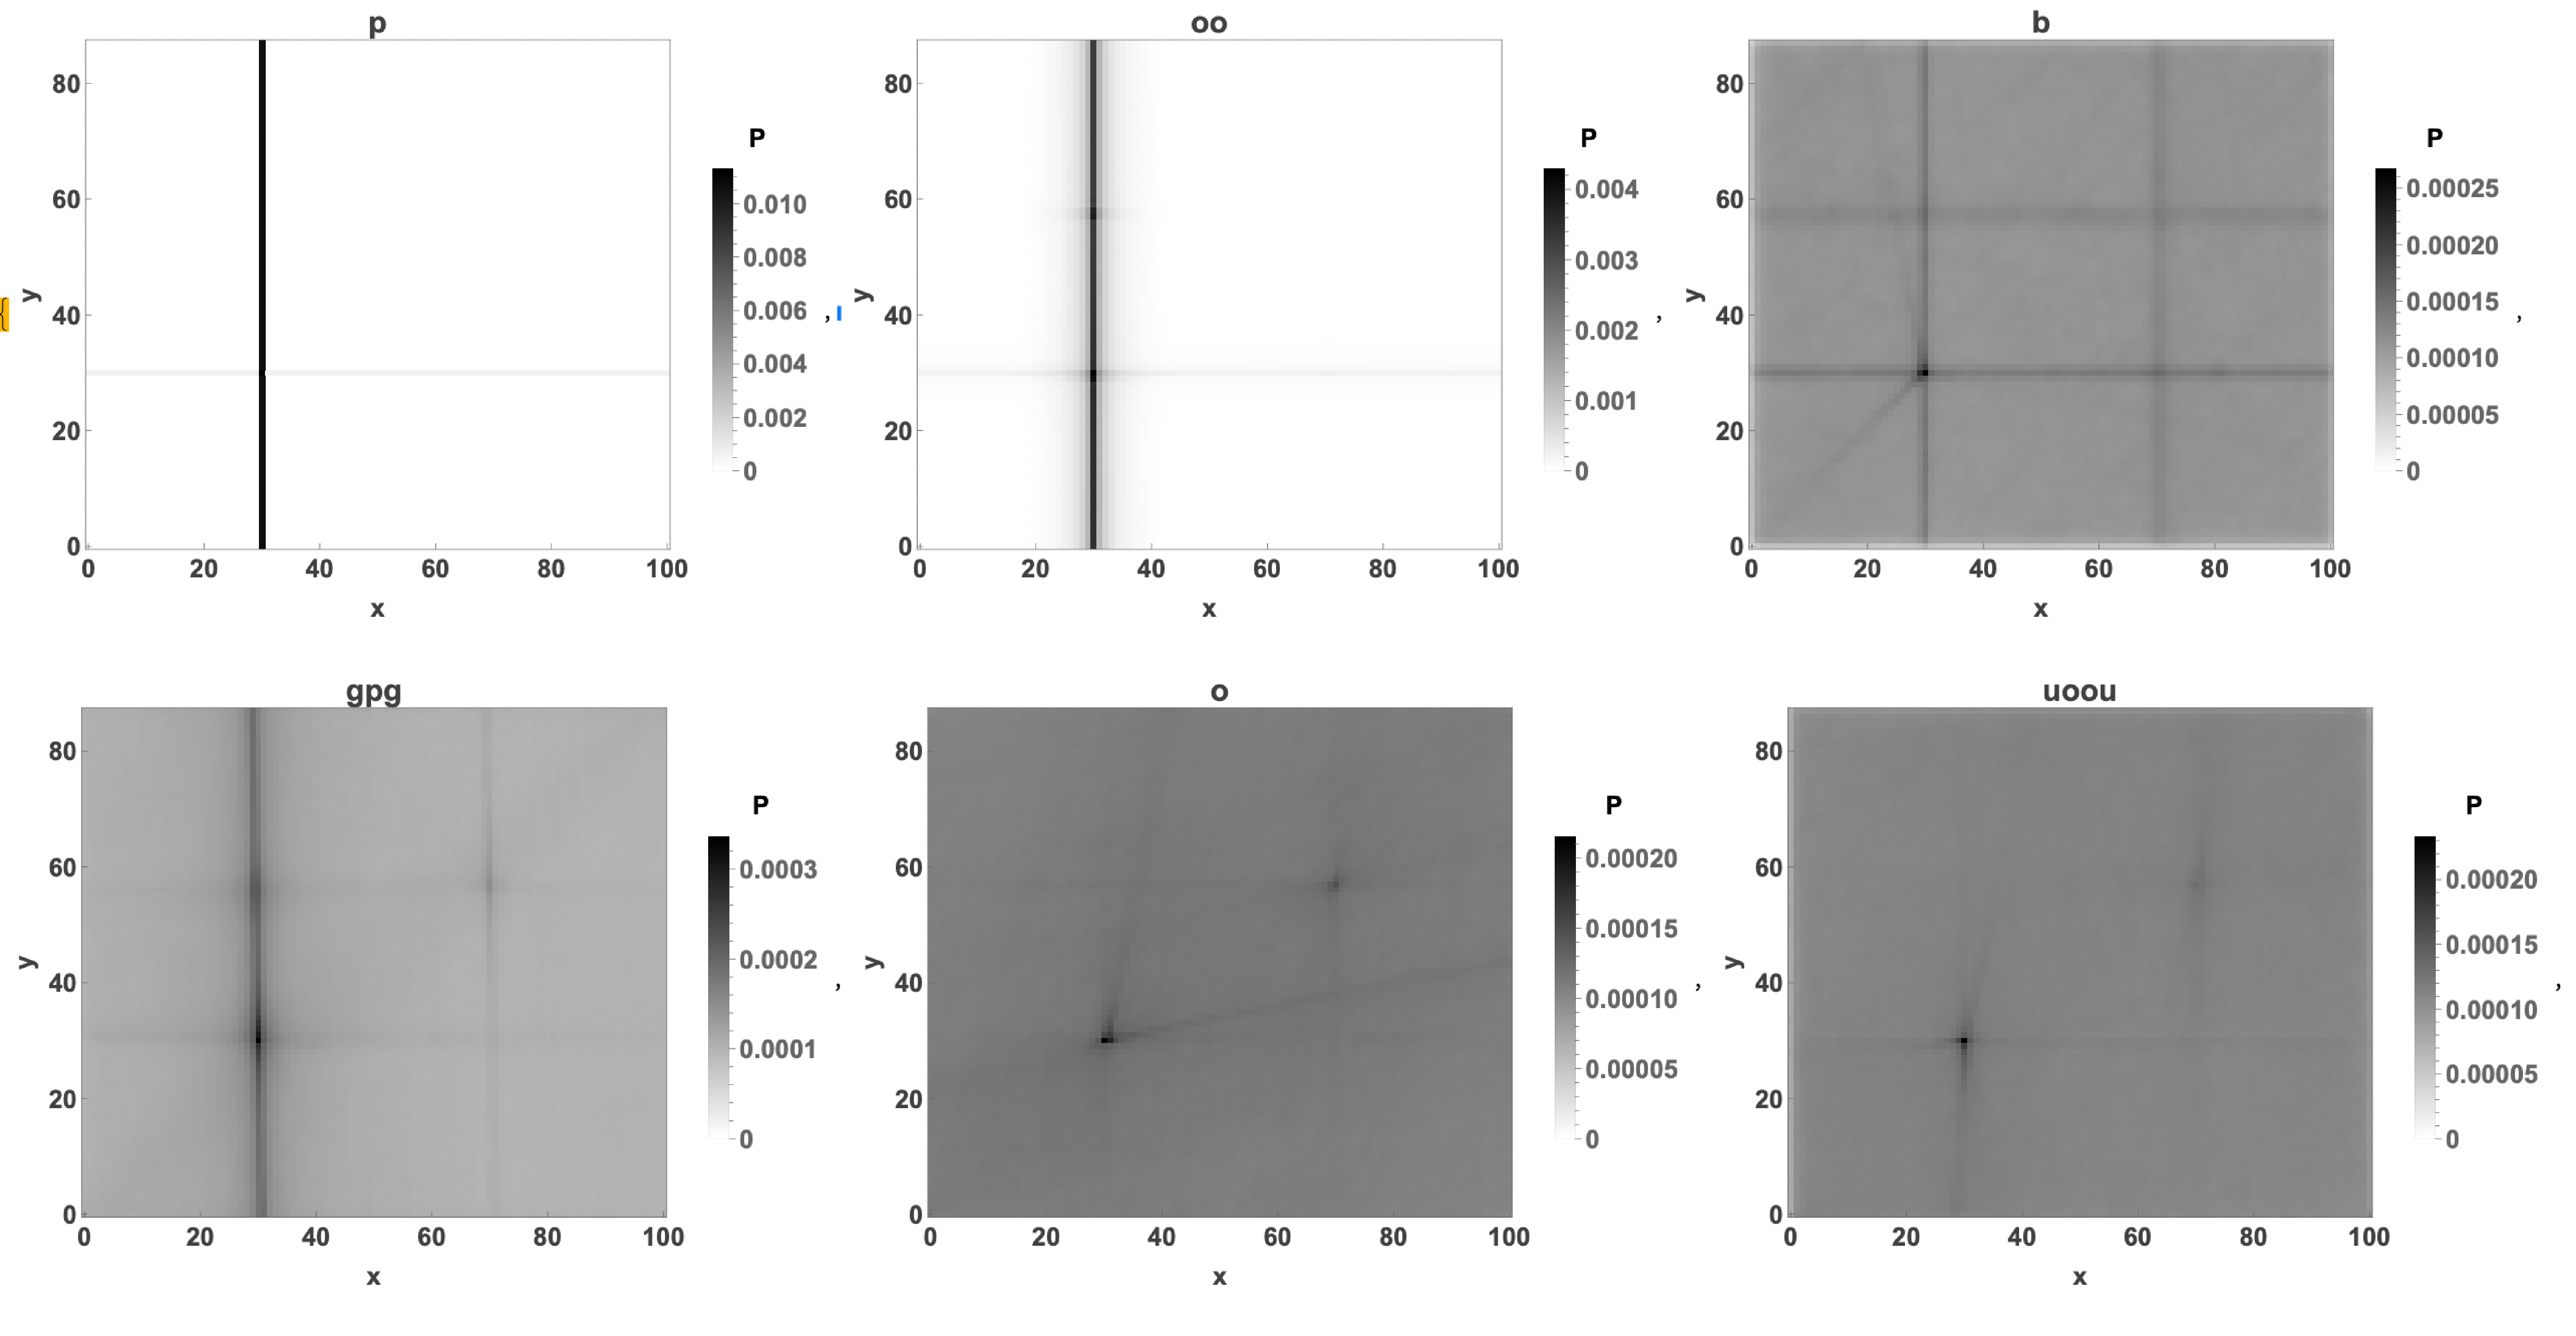
\includegraphics[trim={0.000bp 0.000bp 2174.353bp 845.865bp},clip,width=\linewidth,height=#1,keepaspectratio]{TimeAverage_Rect_p-uoou.pdf}}
\expandafter\def\csname TimeRectoo\endcsname#1{%
  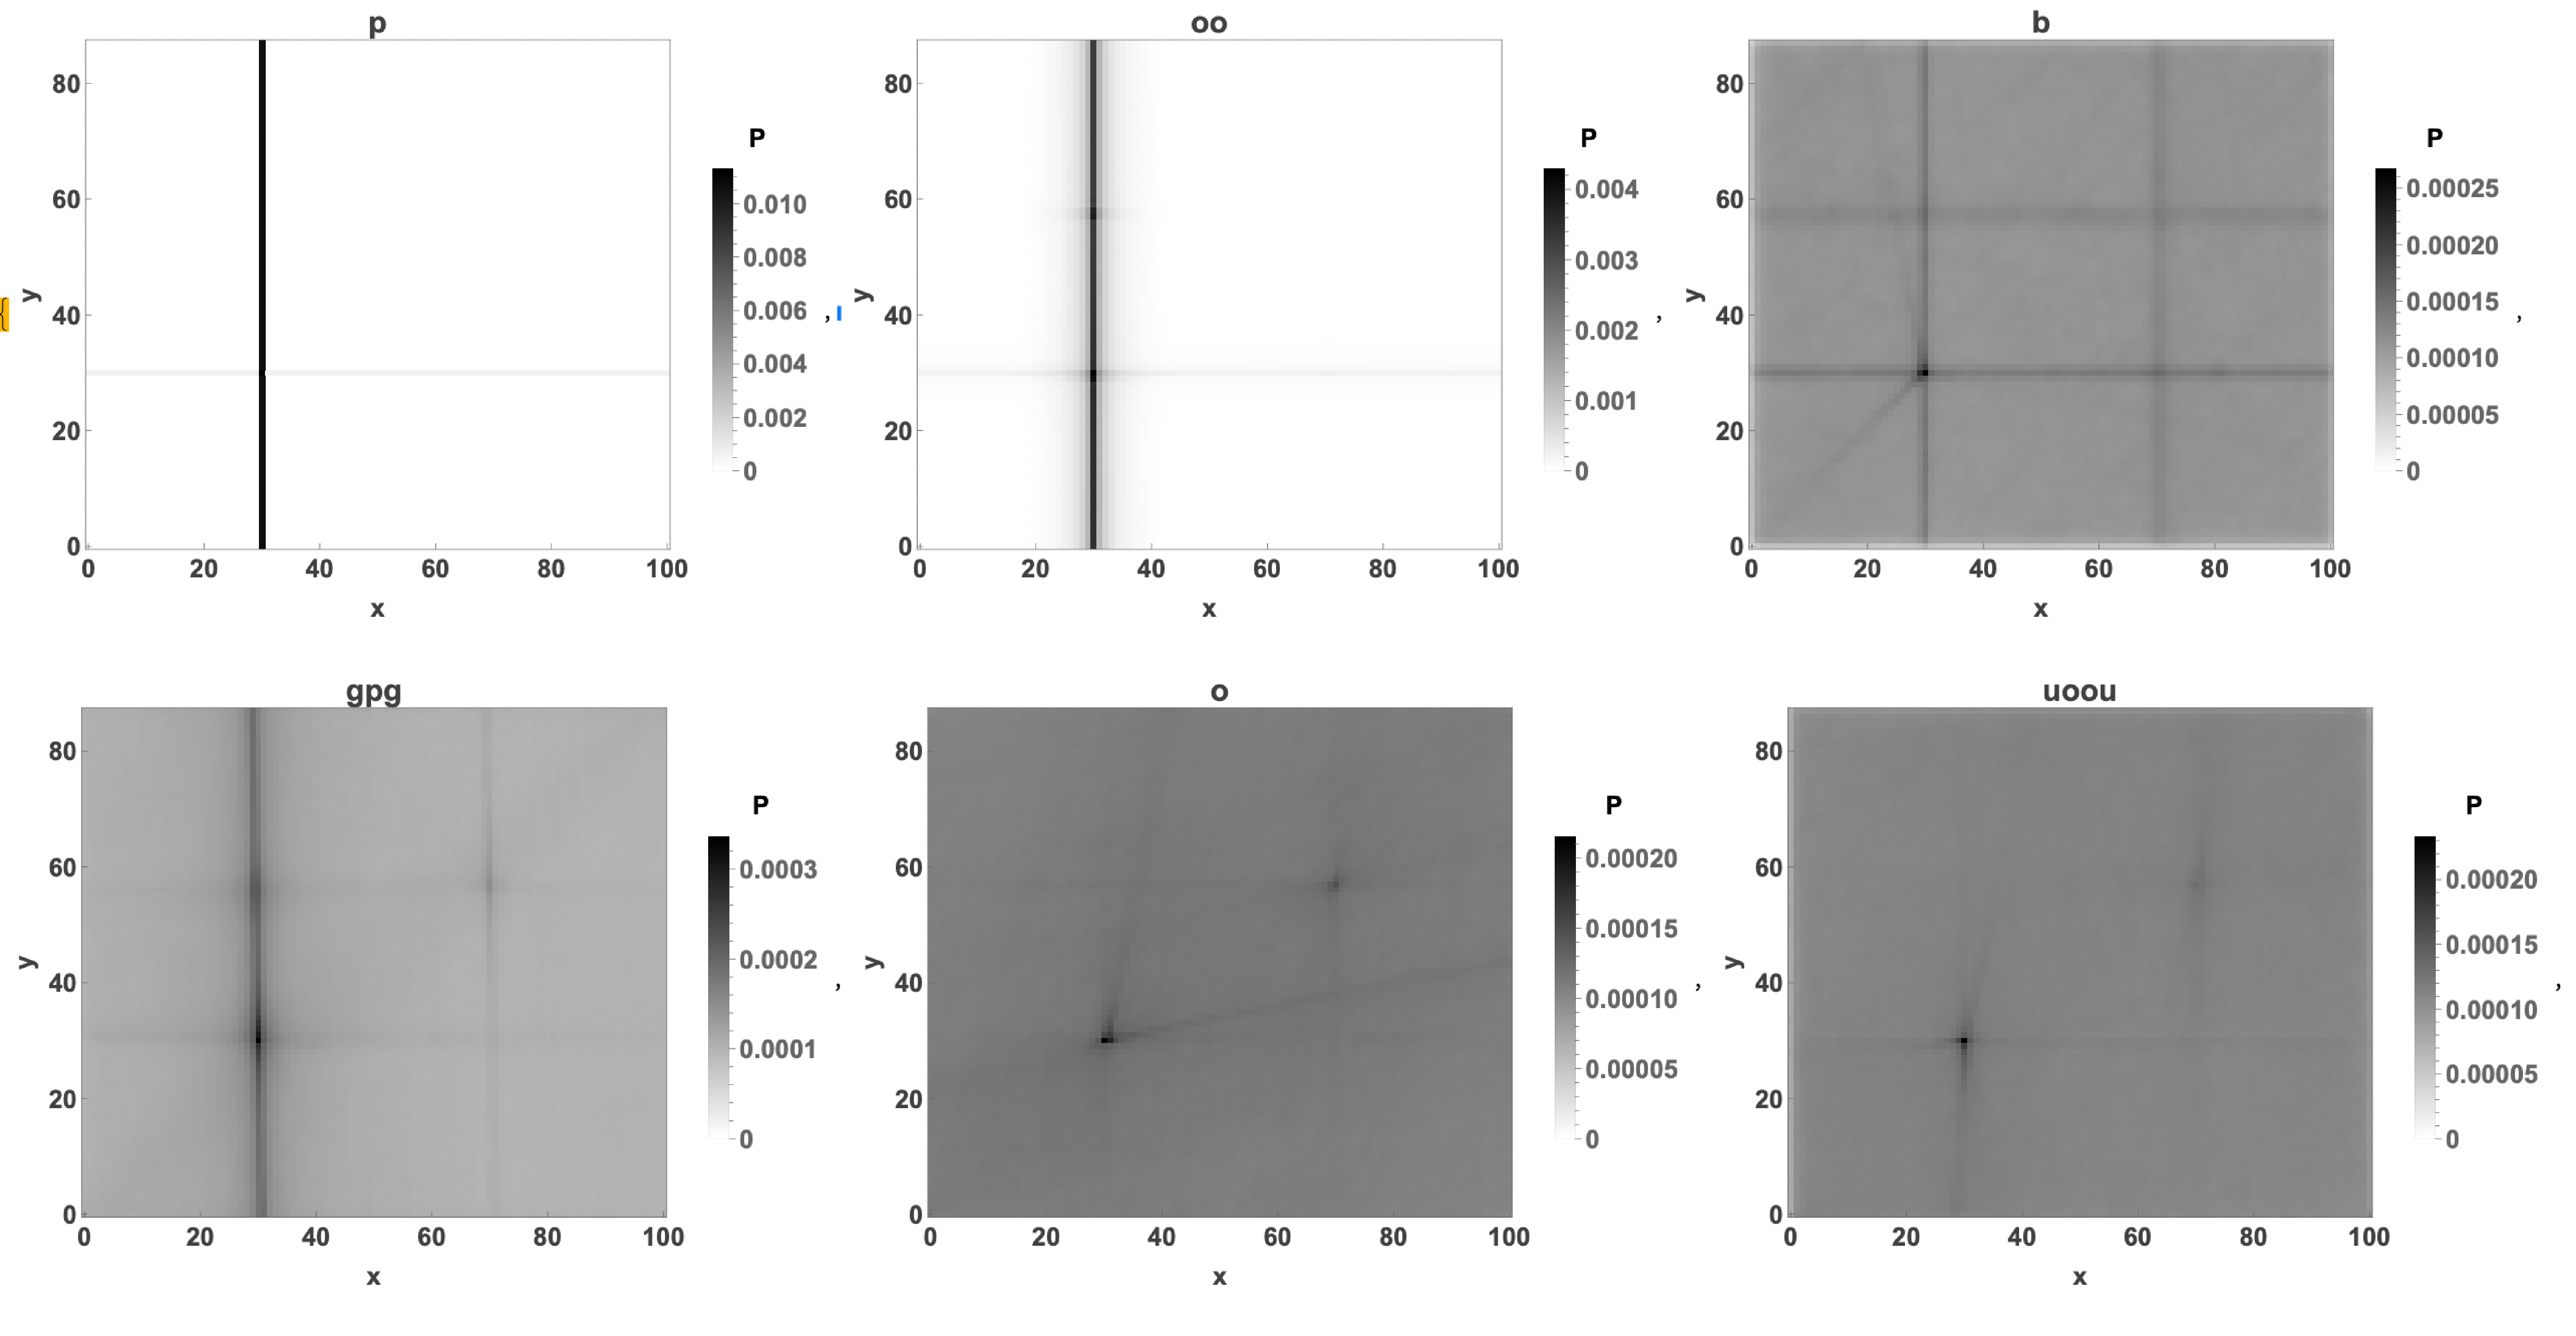
\includegraphics[trim={1087.177bp 845.865bp 1087.177bp 0.000bp},clip,width=\linewidth,height=#1,keepaspectratio]{TimeAverage_Rect_p-uoou.pdf}}
\expandafter\def\csname TimeRectuoou\endcsname#1{%
  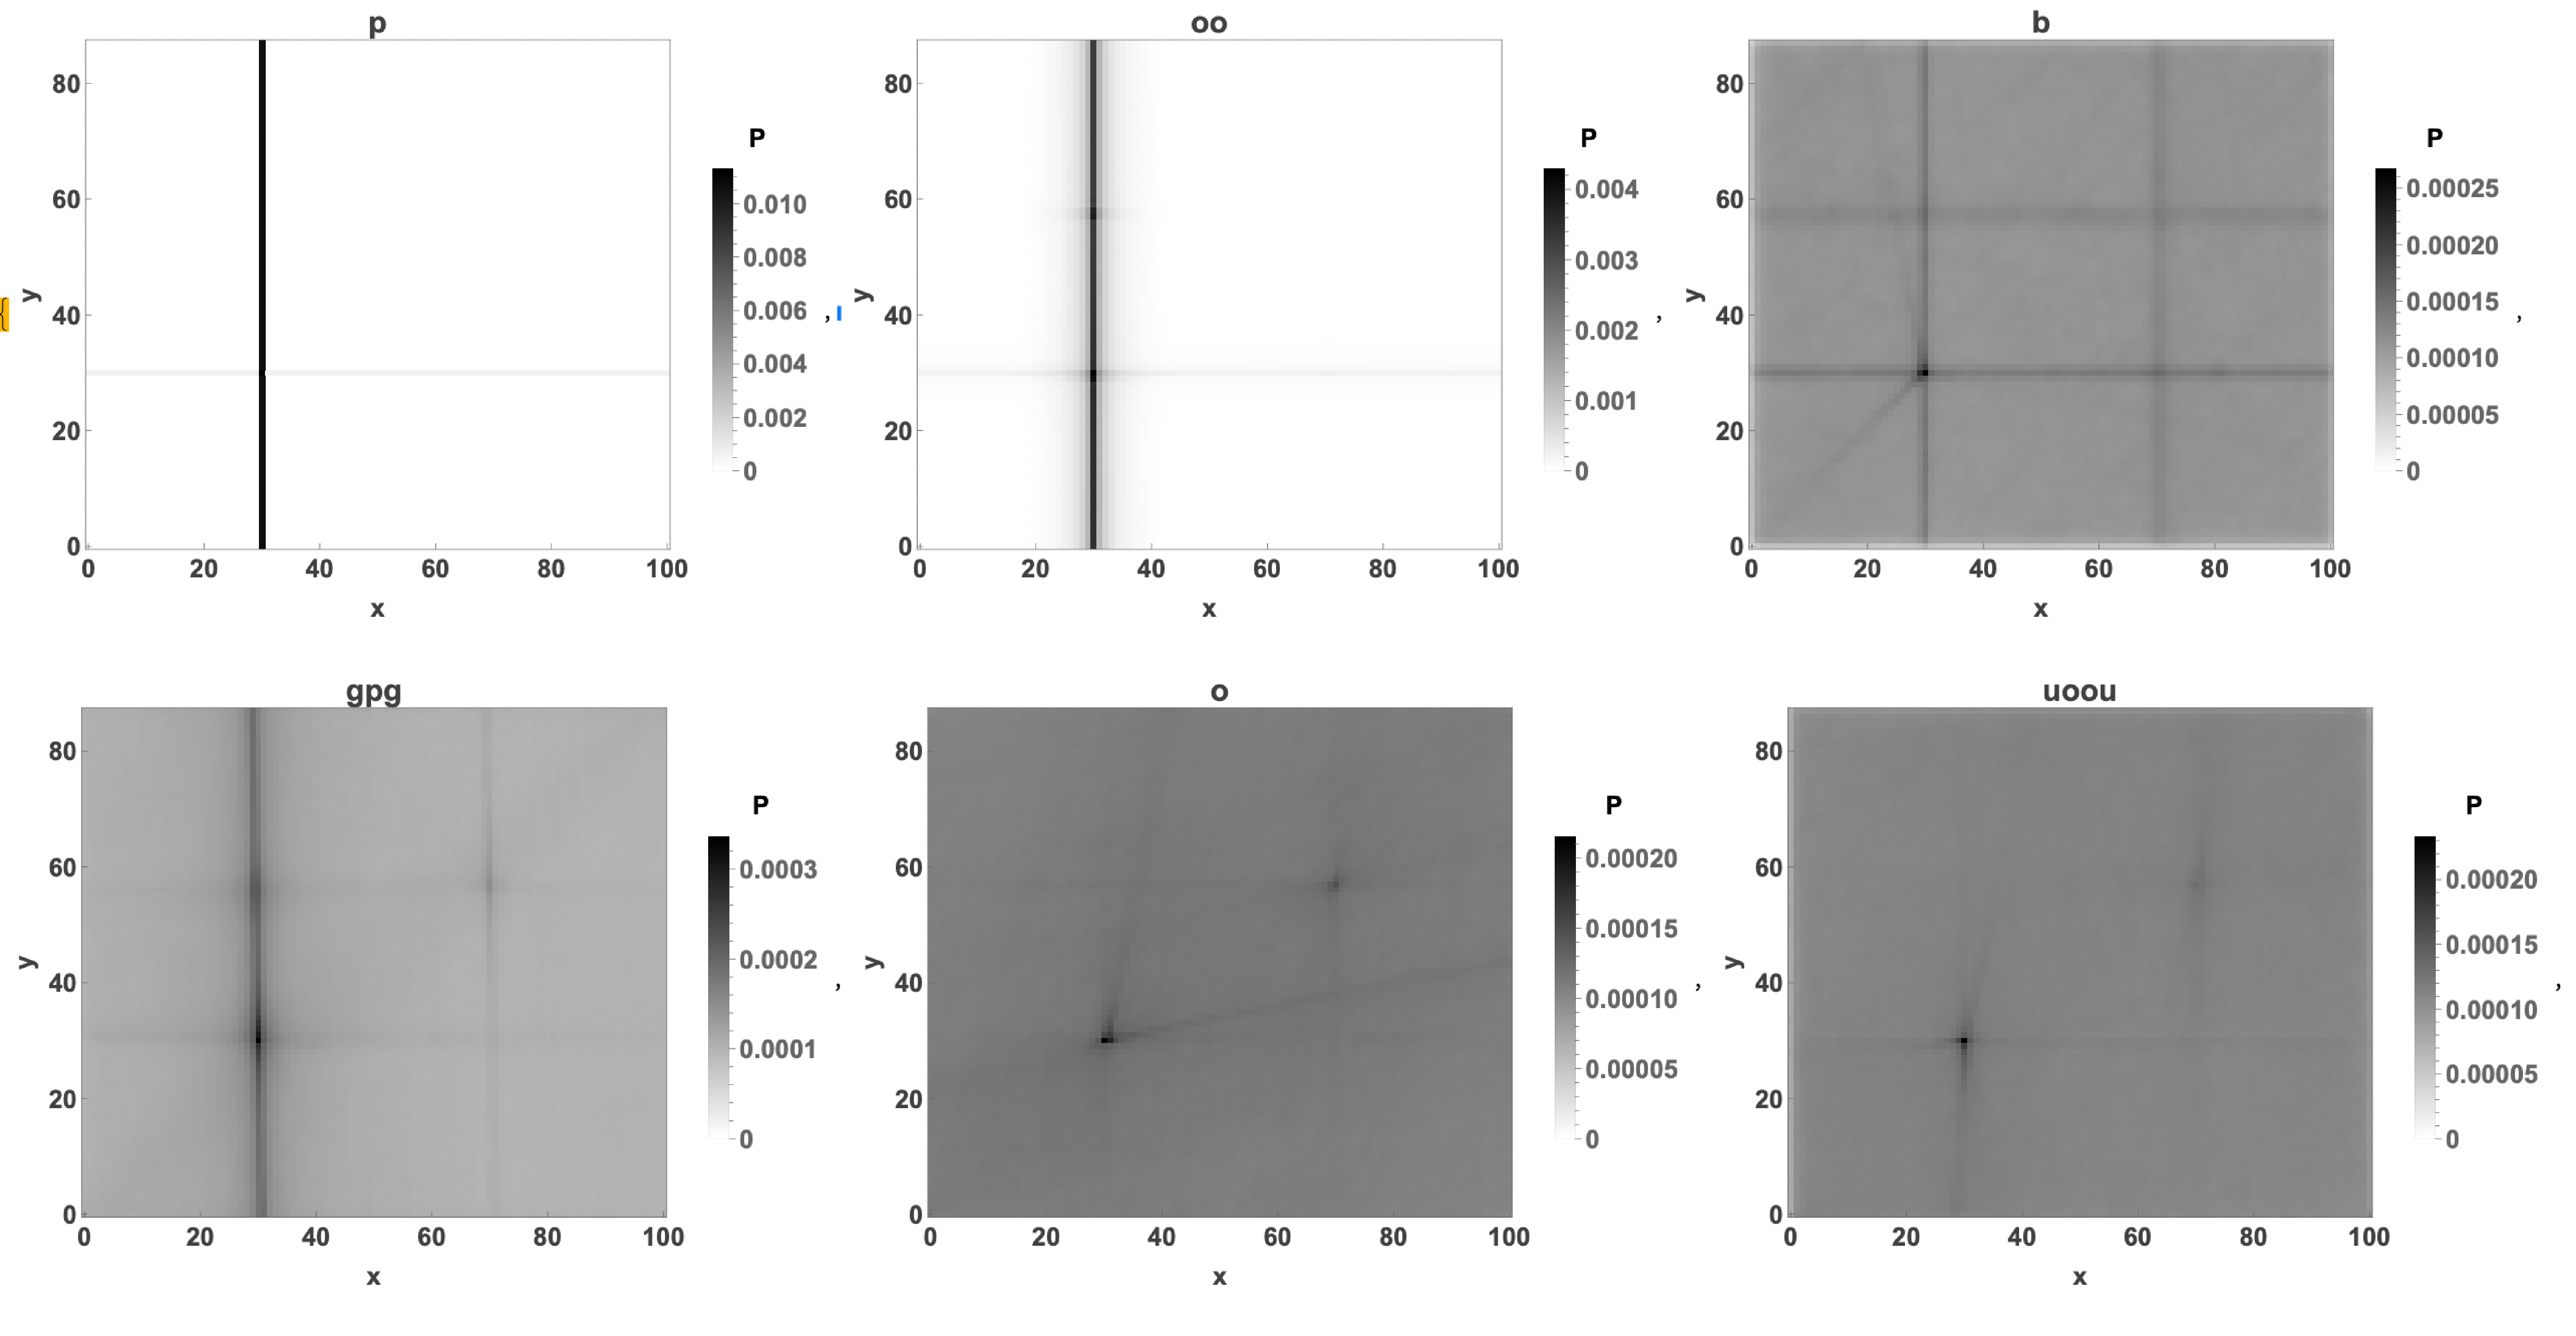
\includegraphics[trim={2174.353bp 0.000bp 0.000bp 845.865bp},clip,width=\linewidth,height=#1,keepaspectratio]{TimeAverage_Rect_p-uoou.pdf}}
\expandafter\def\csname TimeRecto\endcsname#1{%
  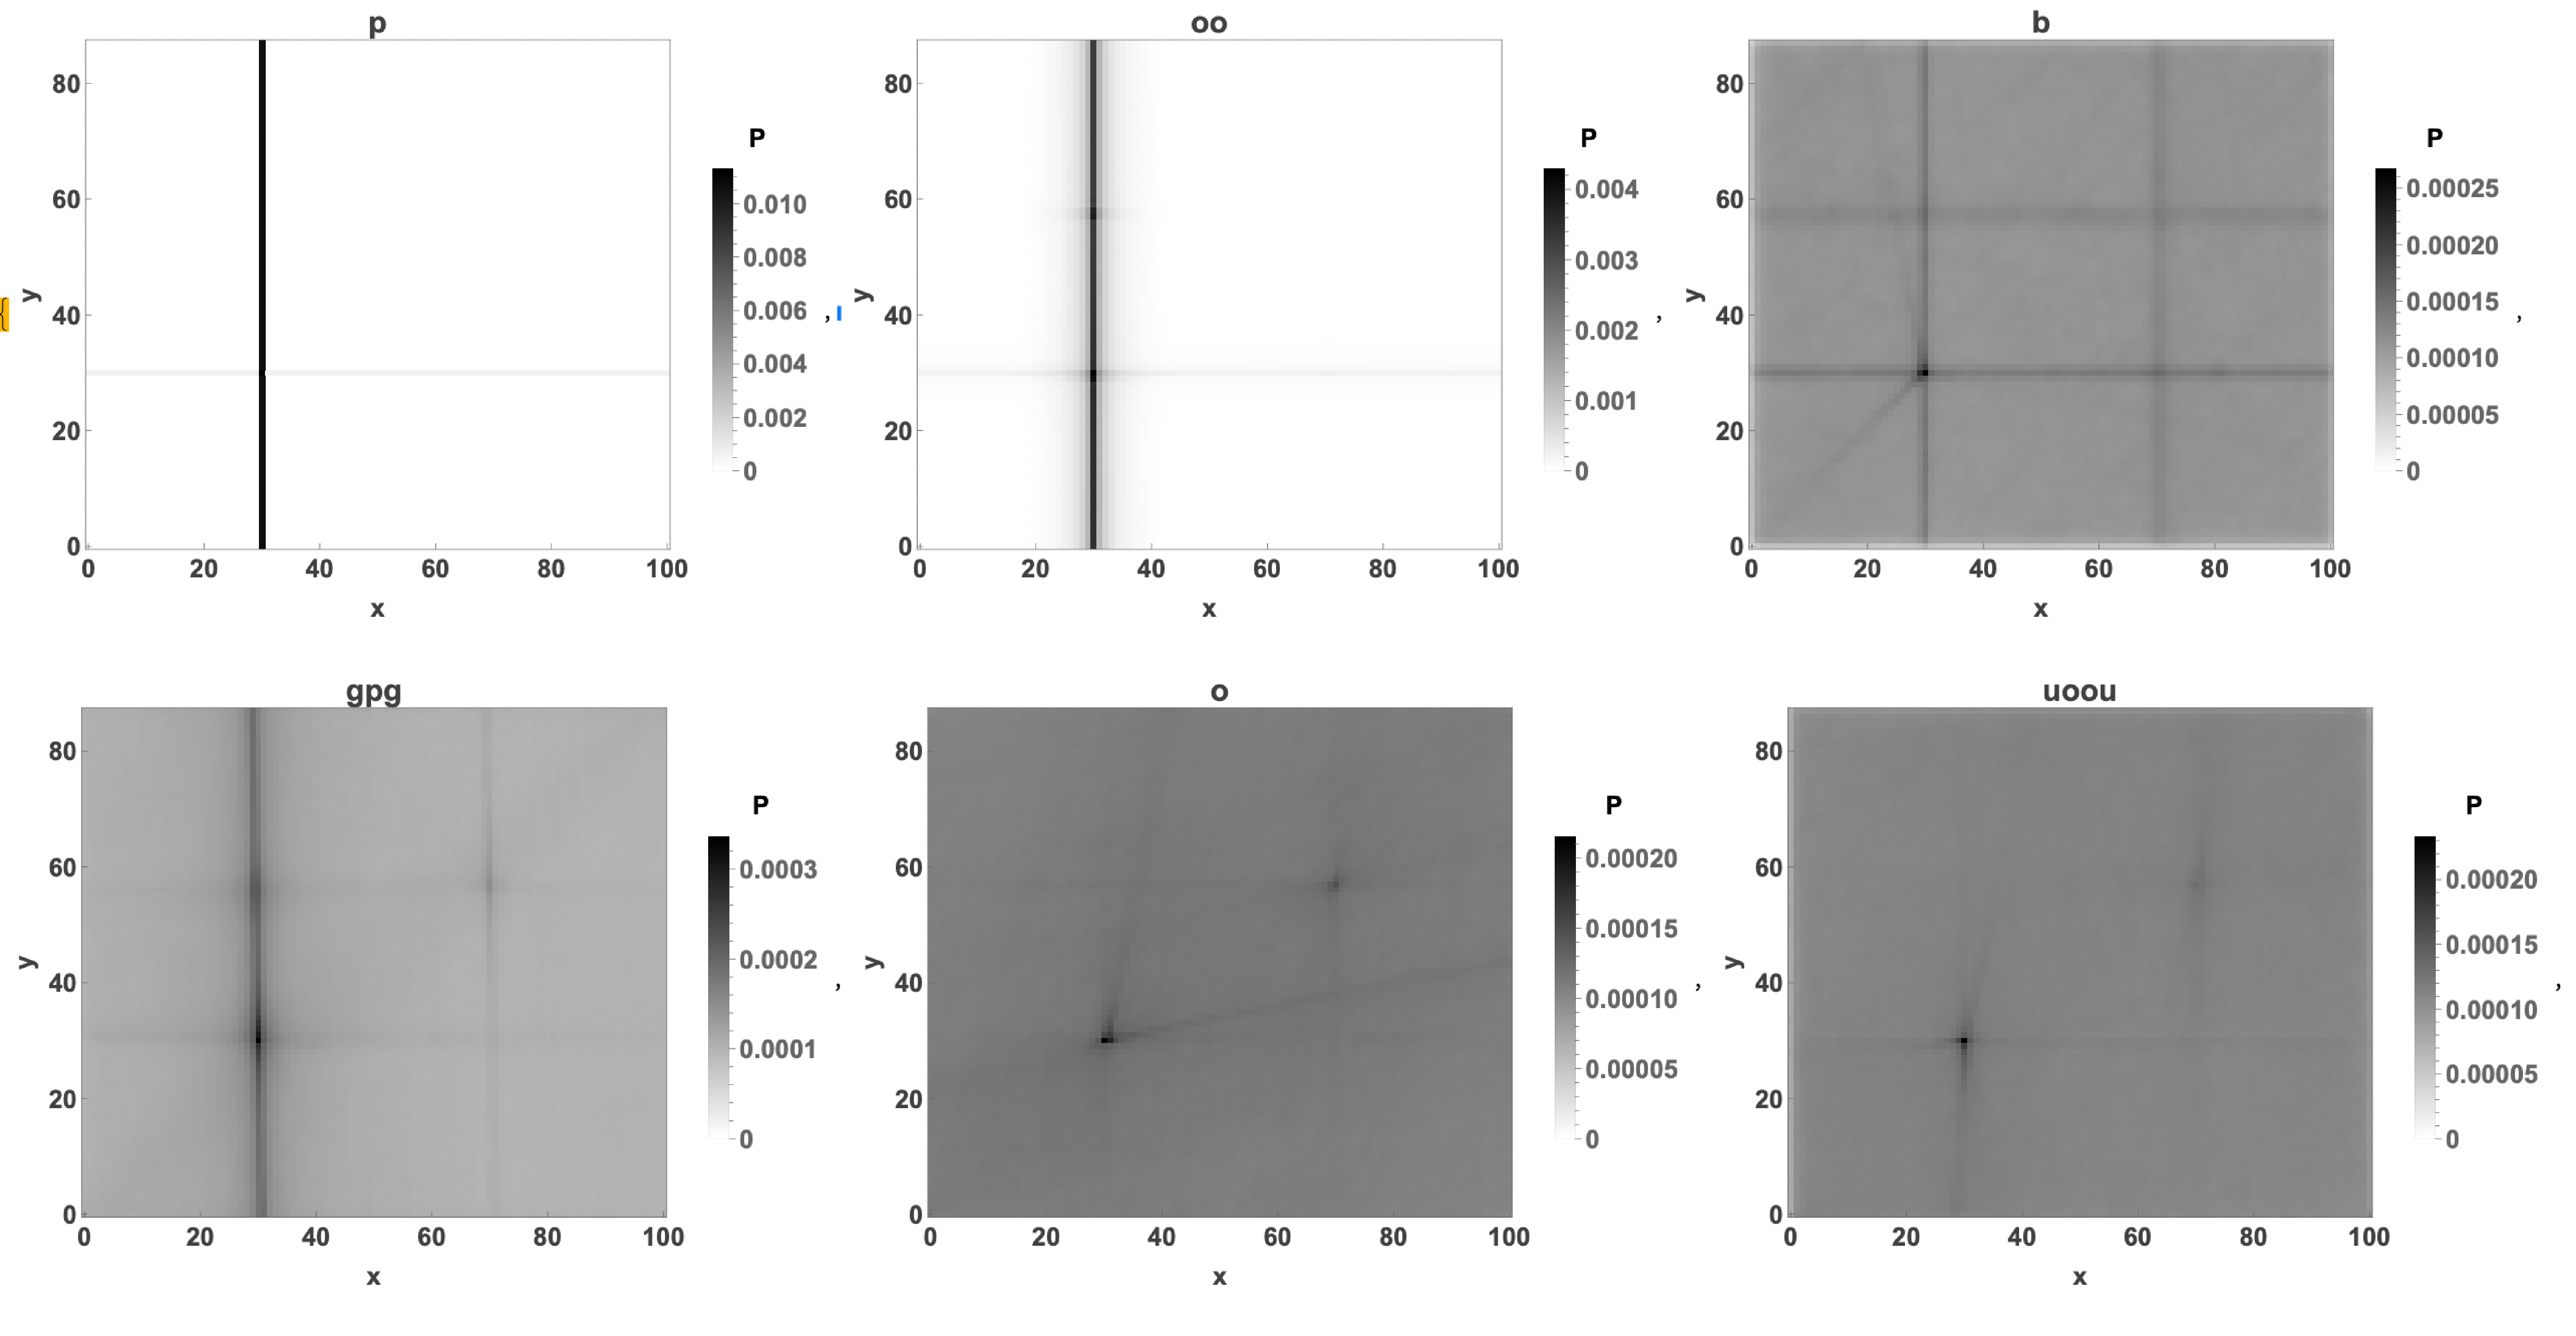
\includegraphics[trim={1087.177bp 0.000bp 1087.177bp 845.865bp},clip,width=\linewidth,height=#1,keepaspectratio]{TimeAverage_Rect_p-uoou.pdf}}
\expandafter\def\csname TimeRectb\endcsname#1{%
  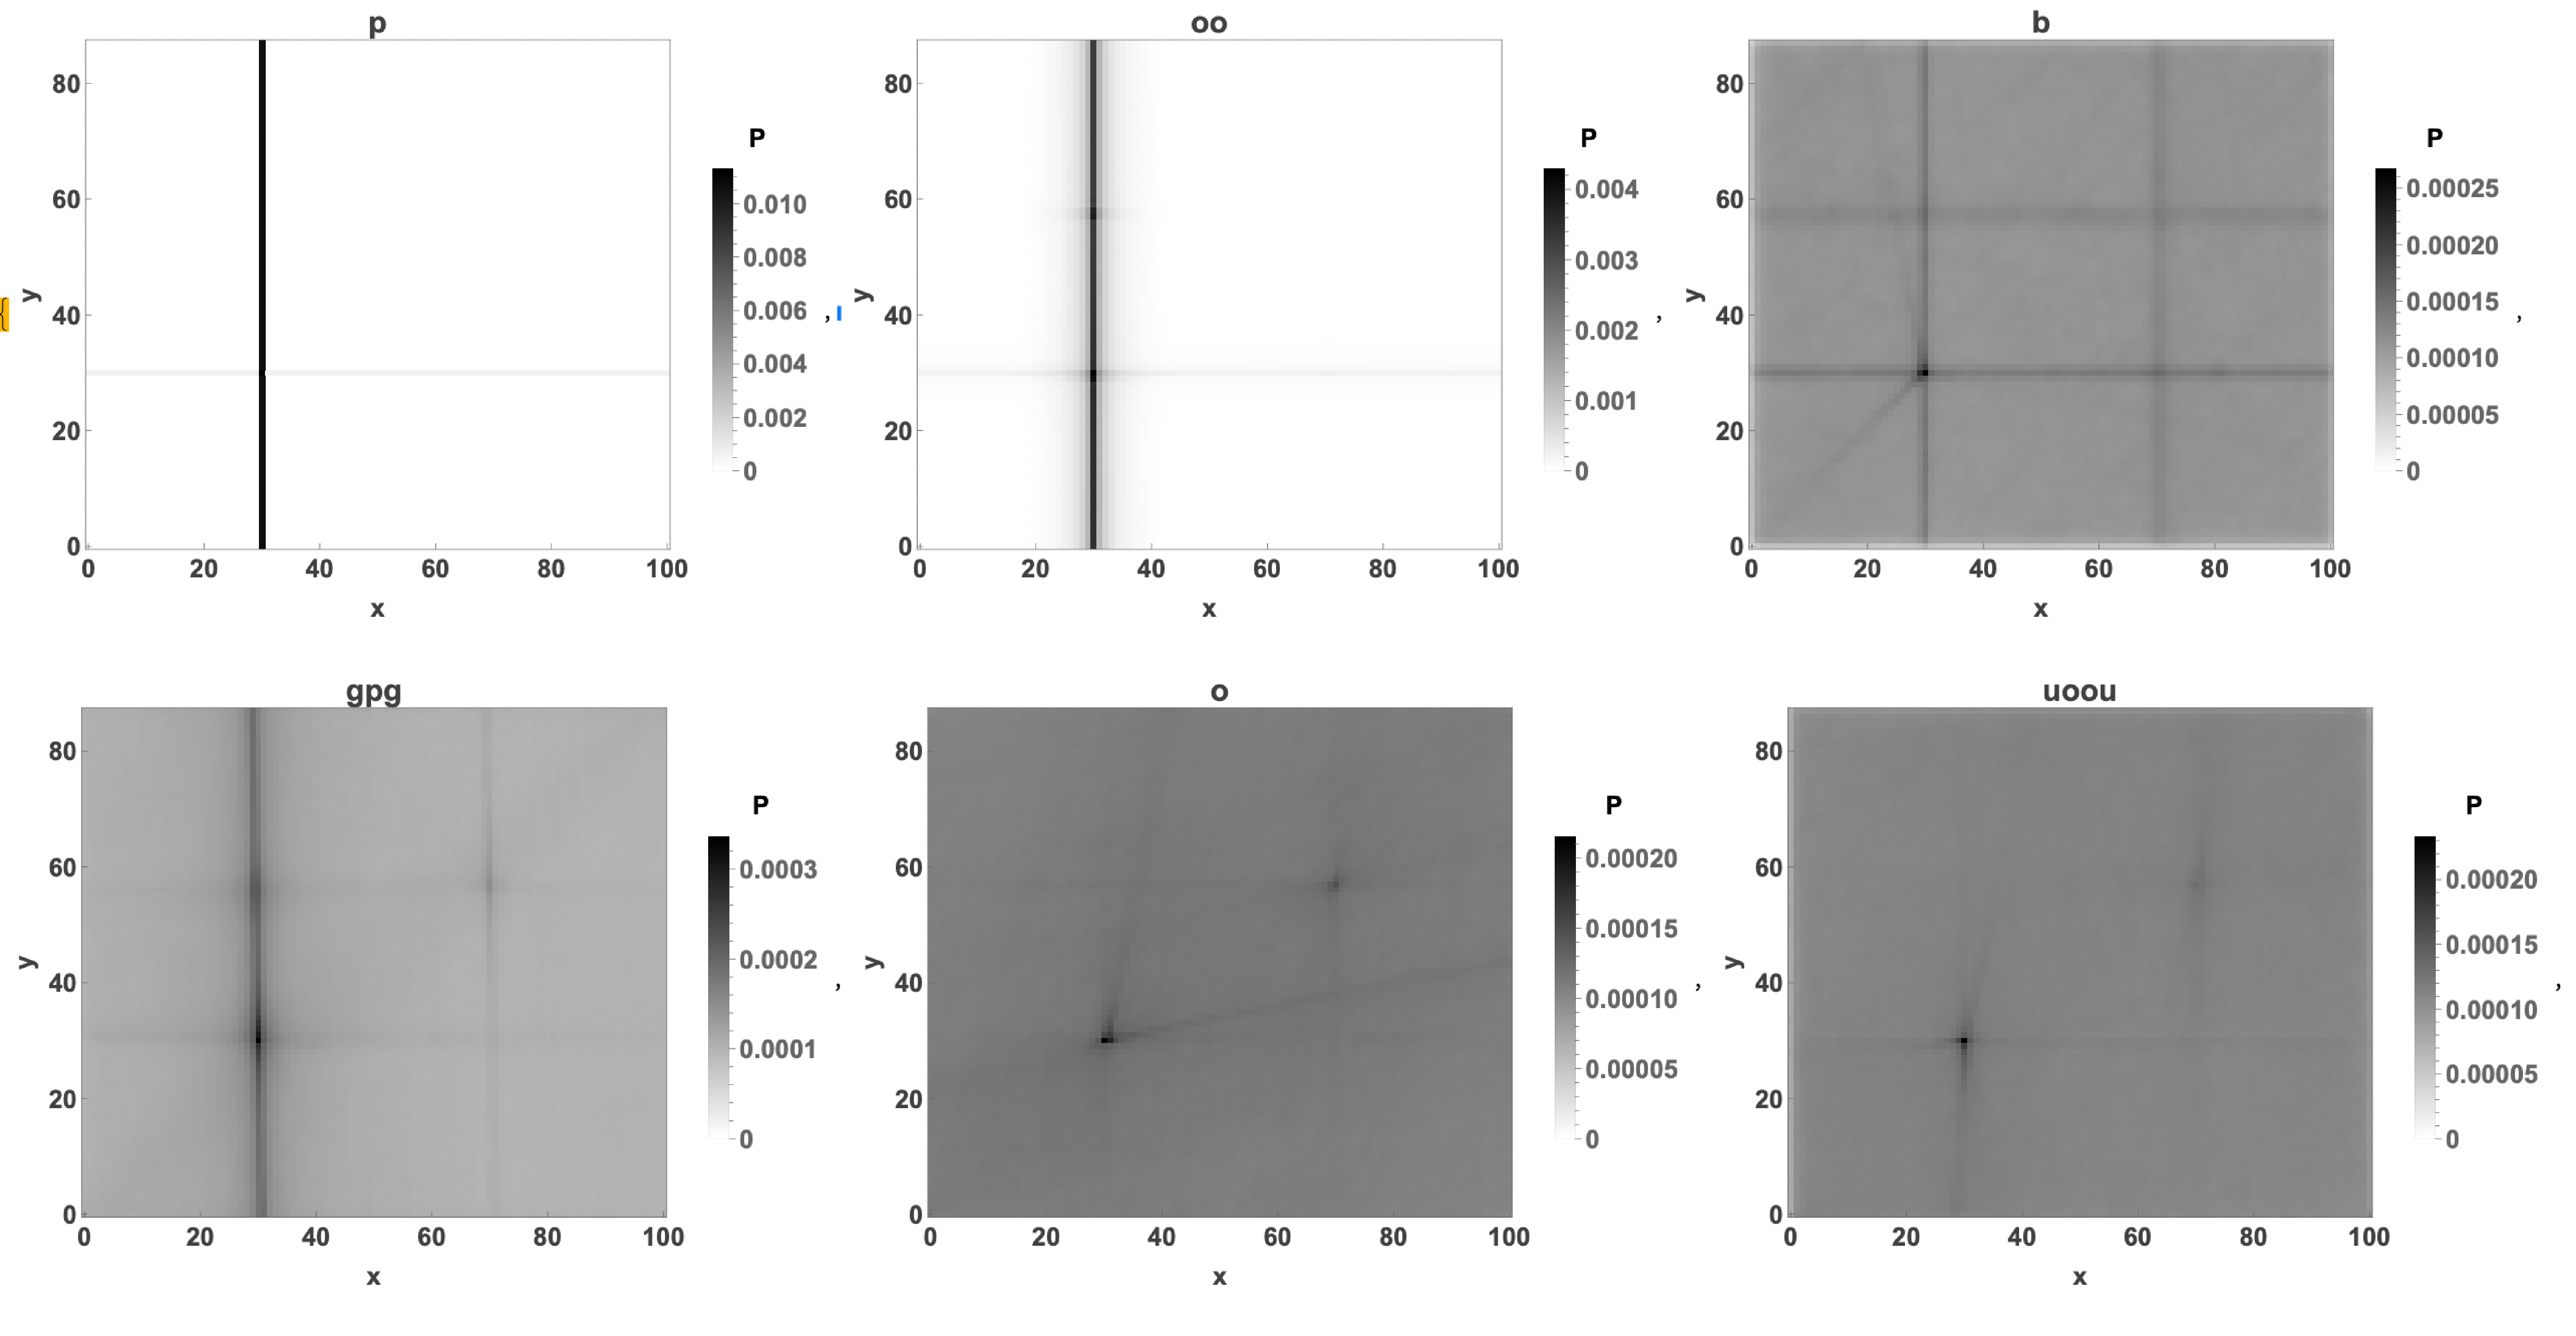
\includegraphics[trim={2174.353bp 845.865bp 0.000bp 0.000bp},clip,width=\linewidth,height=#1,keepaspectratio]{TimeAverage_Rect_p-uoou.pdf}}
\expandafter\def\csname TimeRectubu\endcsname#1{%
  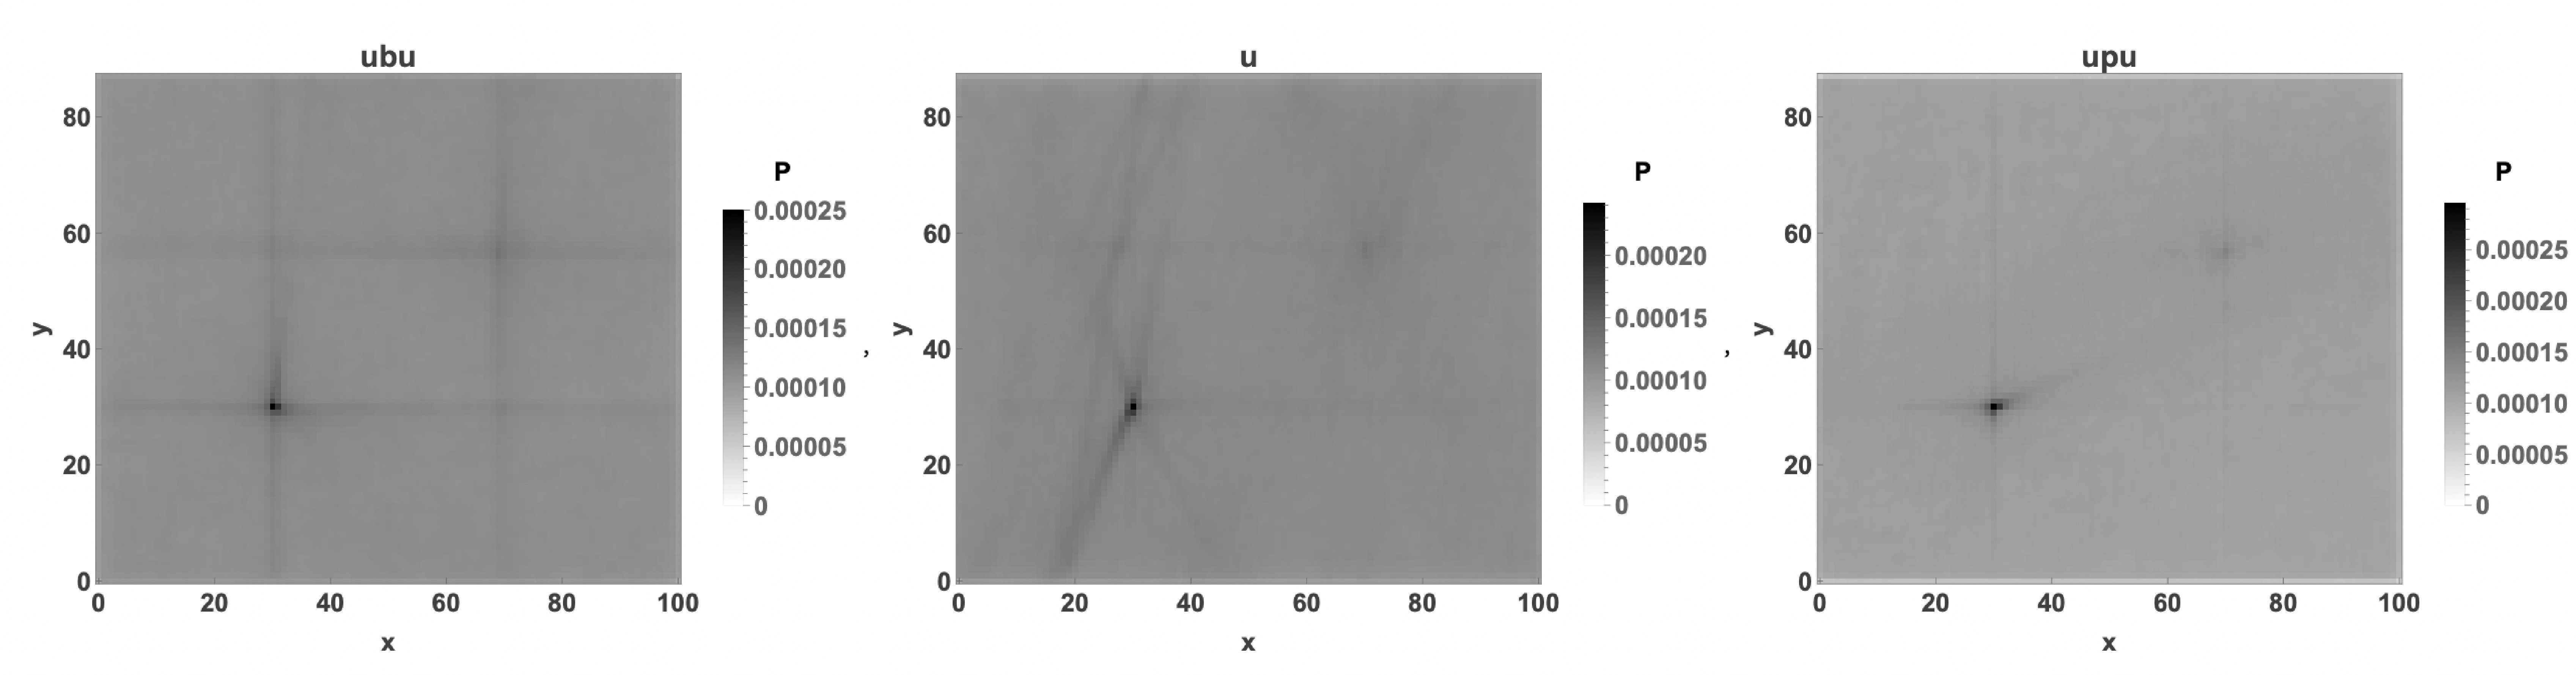
\includegraphics[trim={0.000bp 0.000bp 2172.660bp 0.000bp},clip,width=\linewidth,height=#1,keepaspectratio]{TimeAverage_Rect_ubu-upu.pdf}}
\expandafter\def\csname TimeRectu\endcsname#1{%
  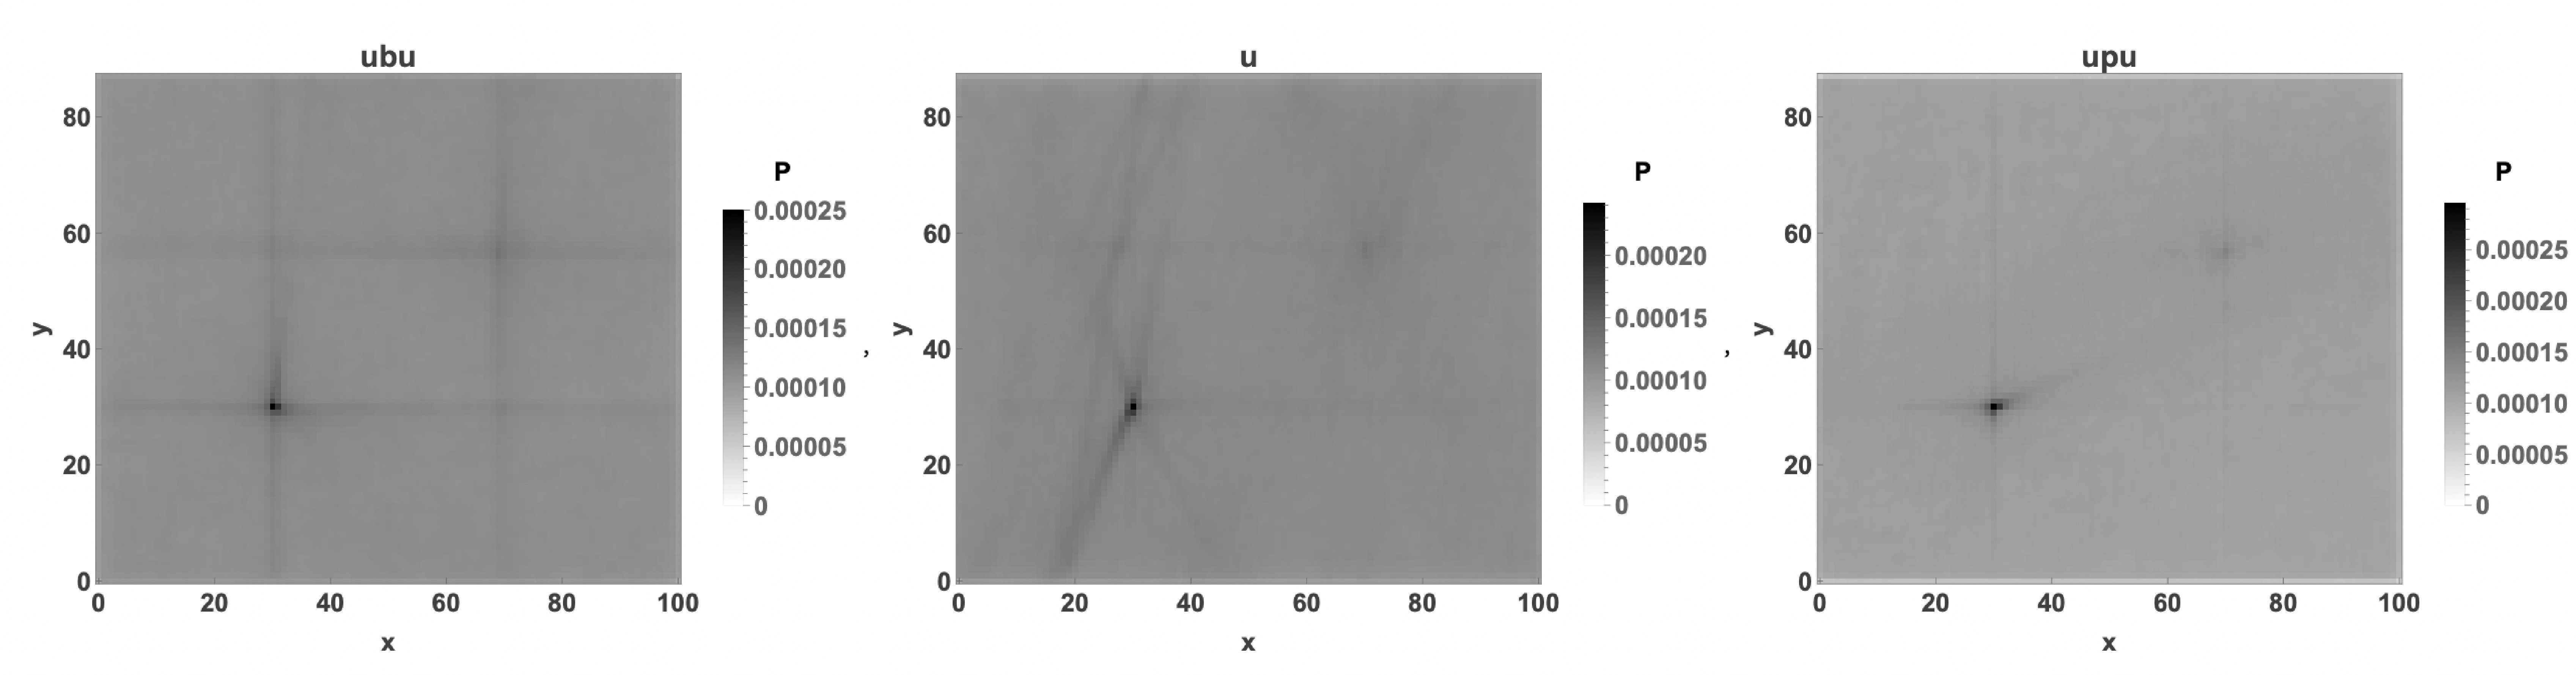
\includegraphics[trim={1086.330bp 0.000bp 1086.330bp 0.000bp},clip,width=\linewidth,height=#1,keepaspectratio]{TimeAverage_Rect_ubu-upu.pdf}}
\expandafter\def\csname TimeRectupu\endcsname#1{%
  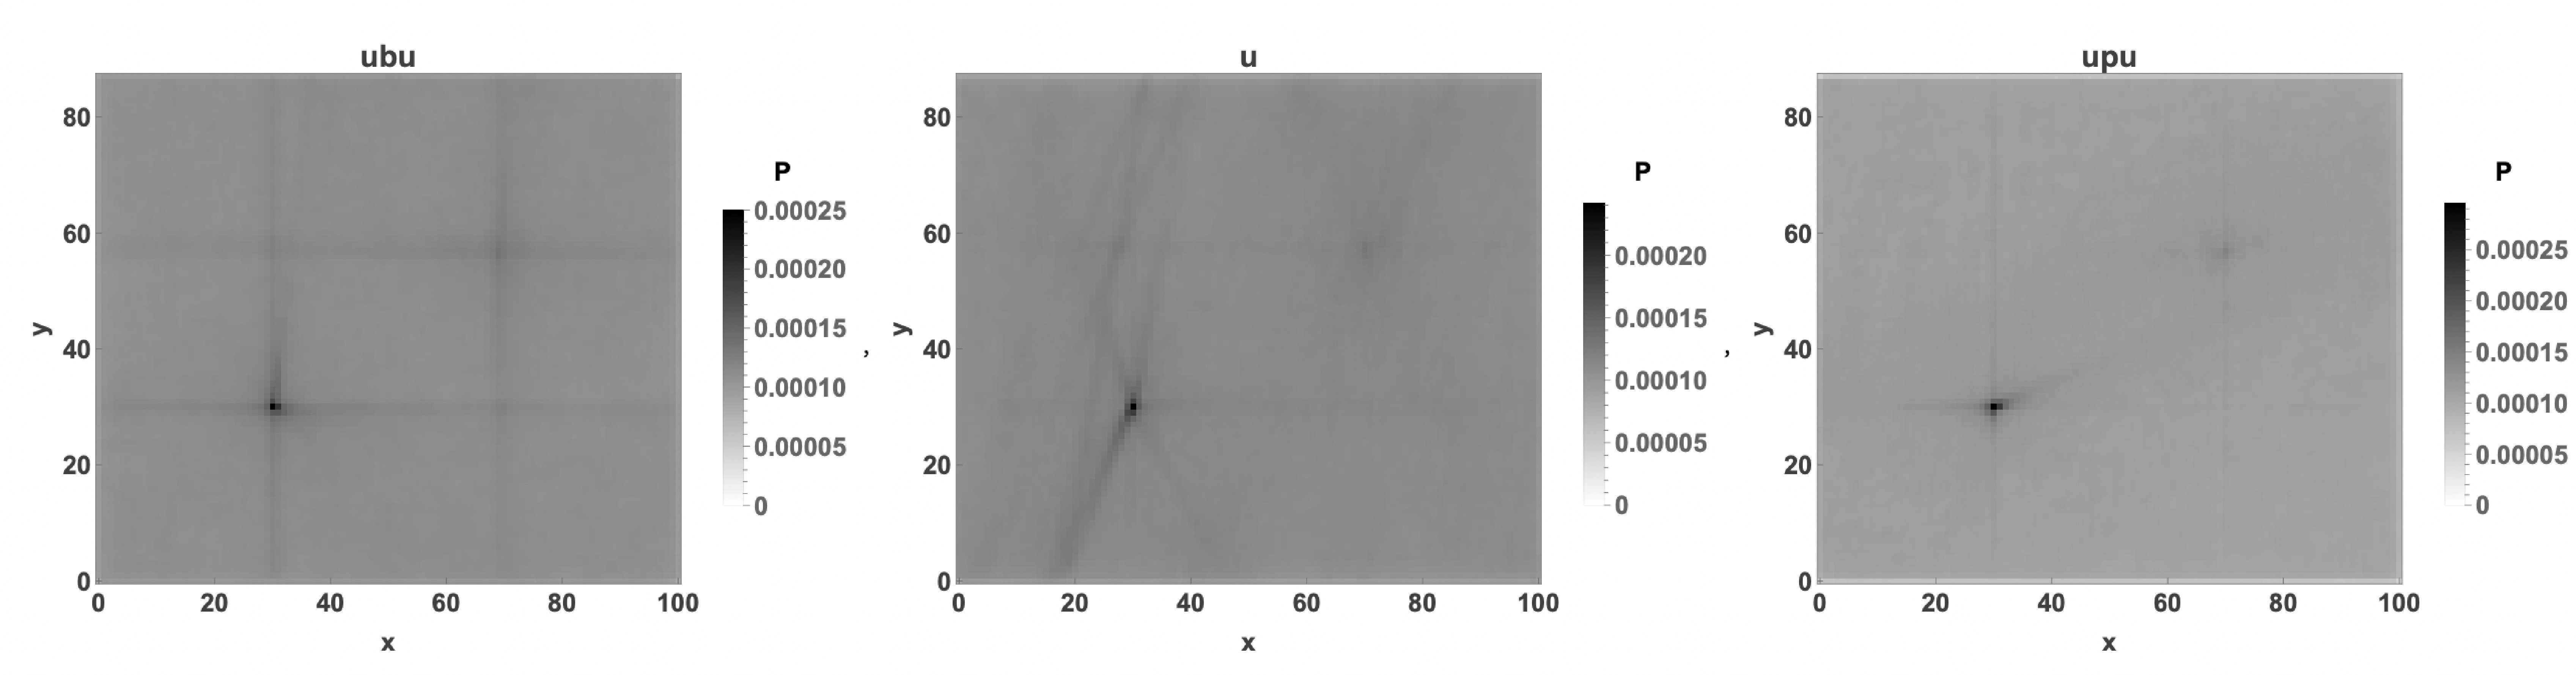
\includegraphics[trim={2172.660bp 0.000bp 0.000bp 0.000bp},clip,width=\linewidth,height=#1,keepaspectratio]{TimeAverage_Rect_ubu-upu.pdf}}
\expandafter\def\csname TimeRectp\endcsname#1{%
  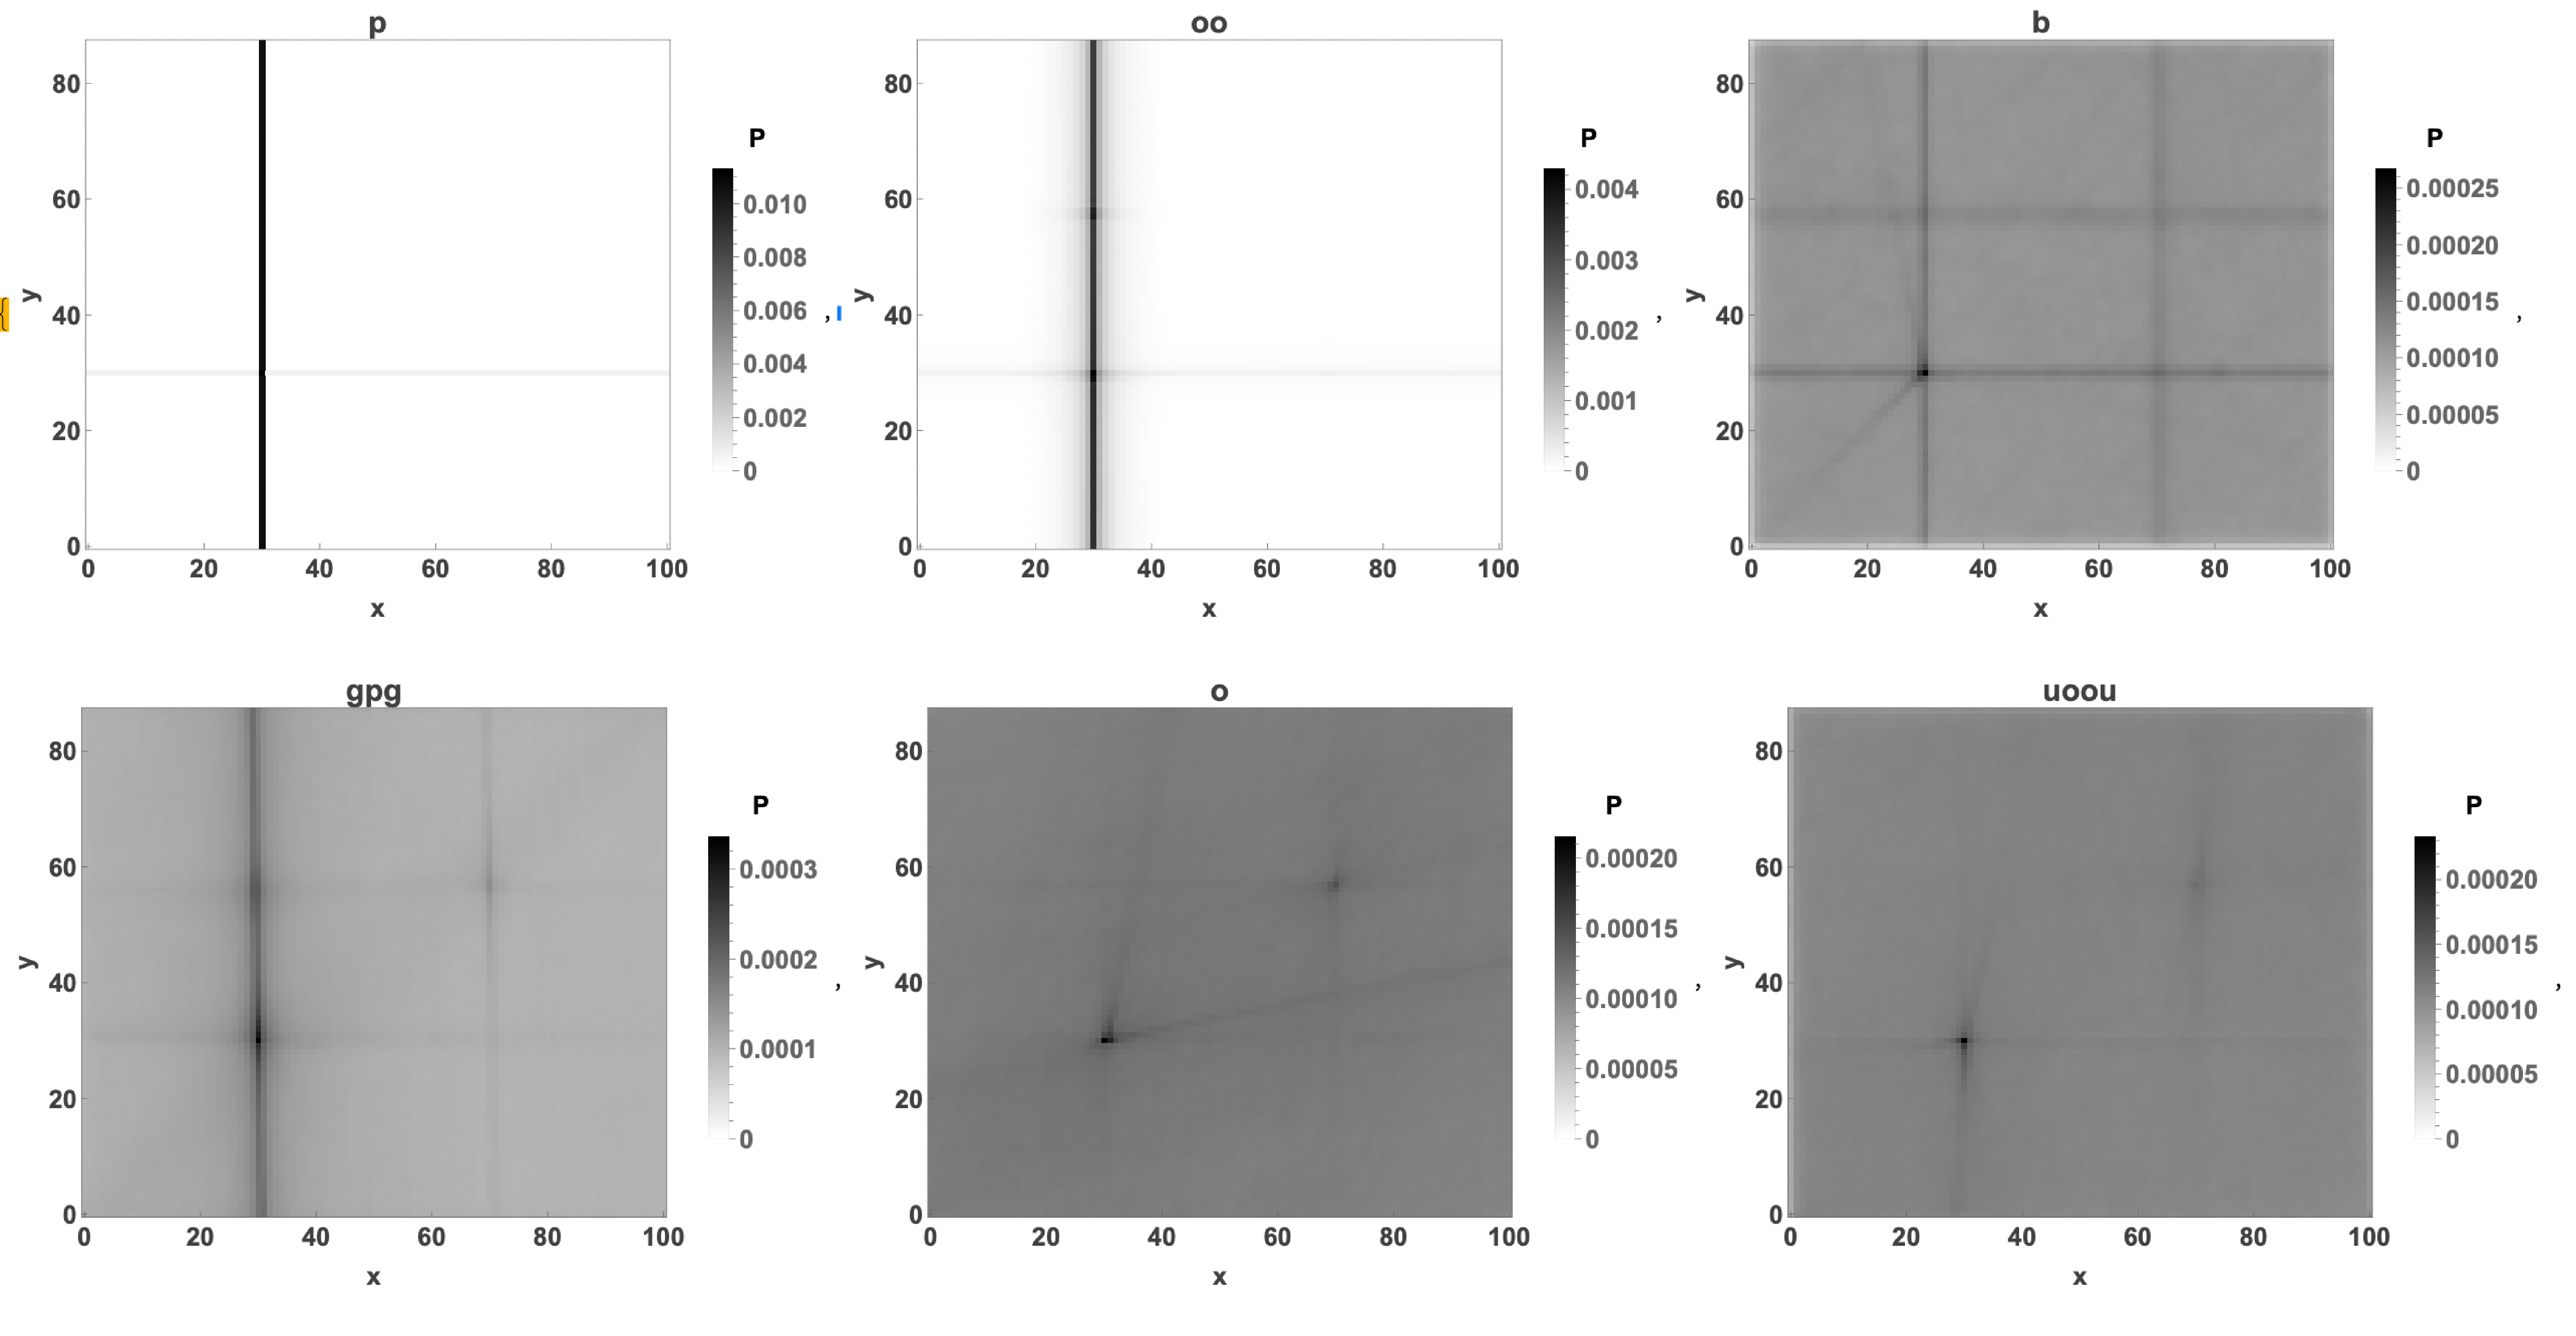
\includegraphics[trim={0.000bp 845.865bp 2174.353bp 0.000bp},clip,width=\linewidth,height=#1,keepaspectratio]{TimeAverage_Rect_p-uoou.pdf}}
\expandafter\def\csname TimeSinaigpg\endcsname#1{%
  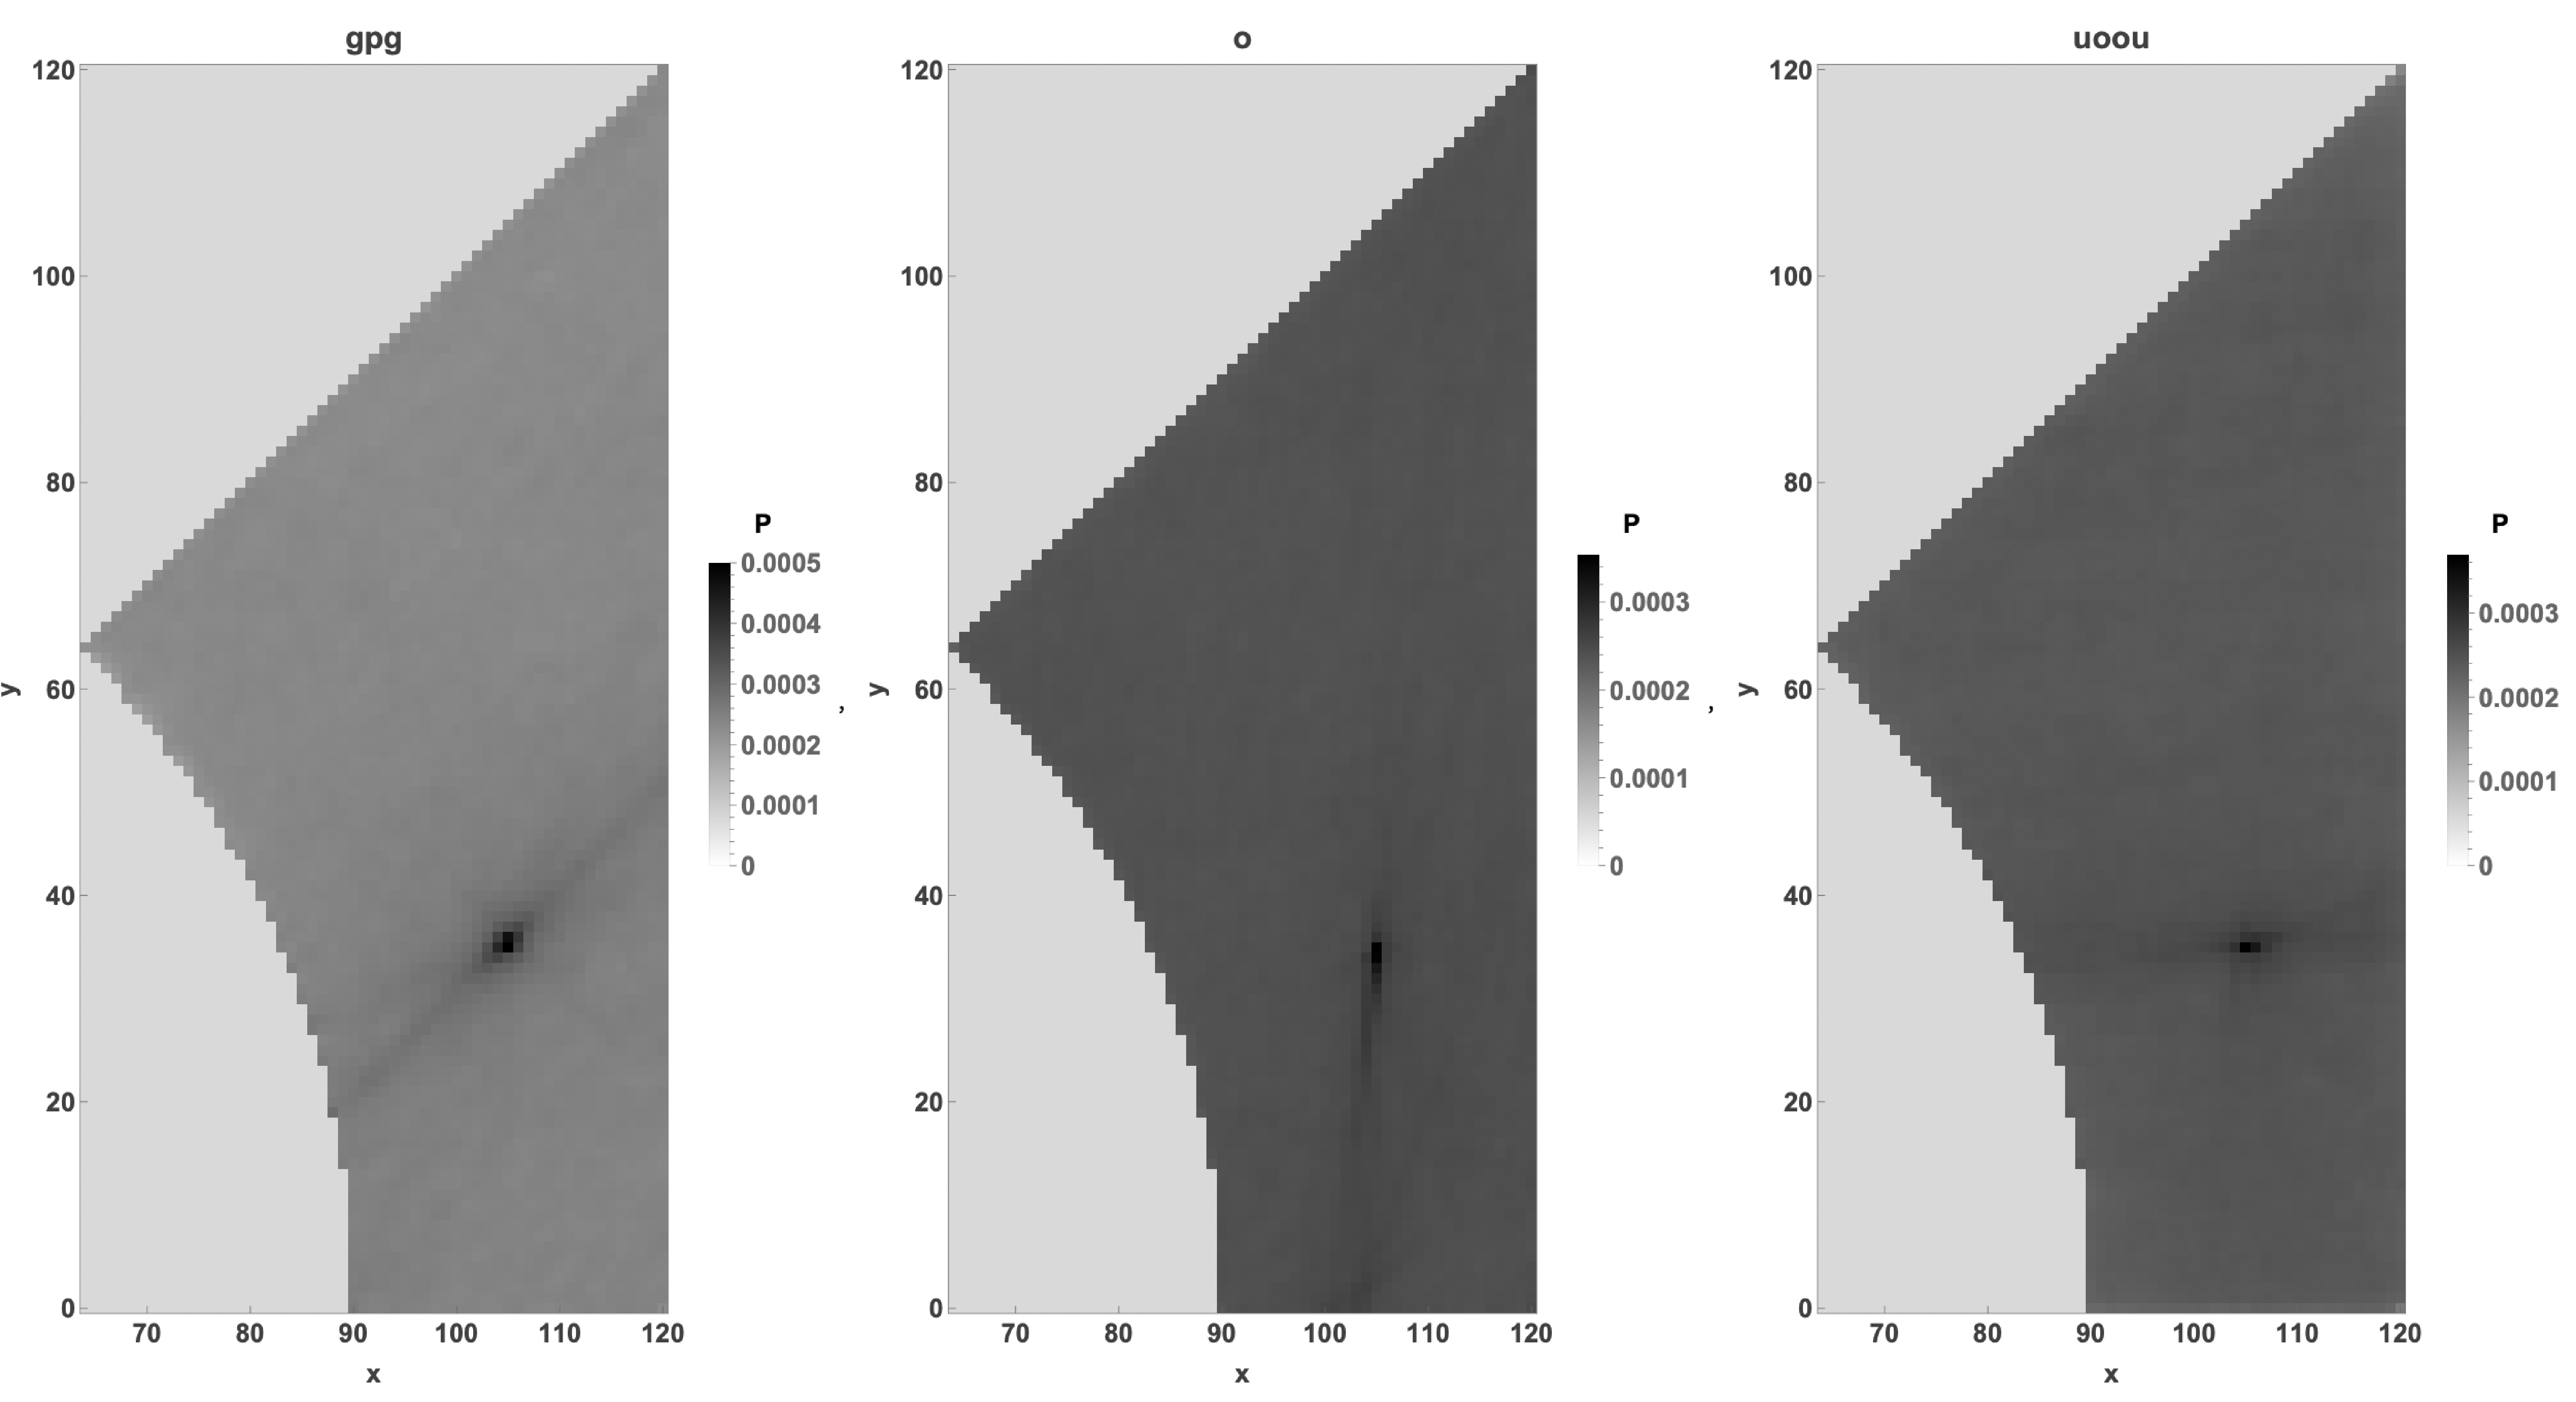
\includegraphics[trim={0.000bp 0.000bp 2116.773bp 0.000bp},clip,width=\linewidth,height=#1,keepaspectratio]{TimeAverage_Sinai_gpg-uoou.pdf}}
\expandafter\def\csname TimeSinaioo\endcsname#1{%
  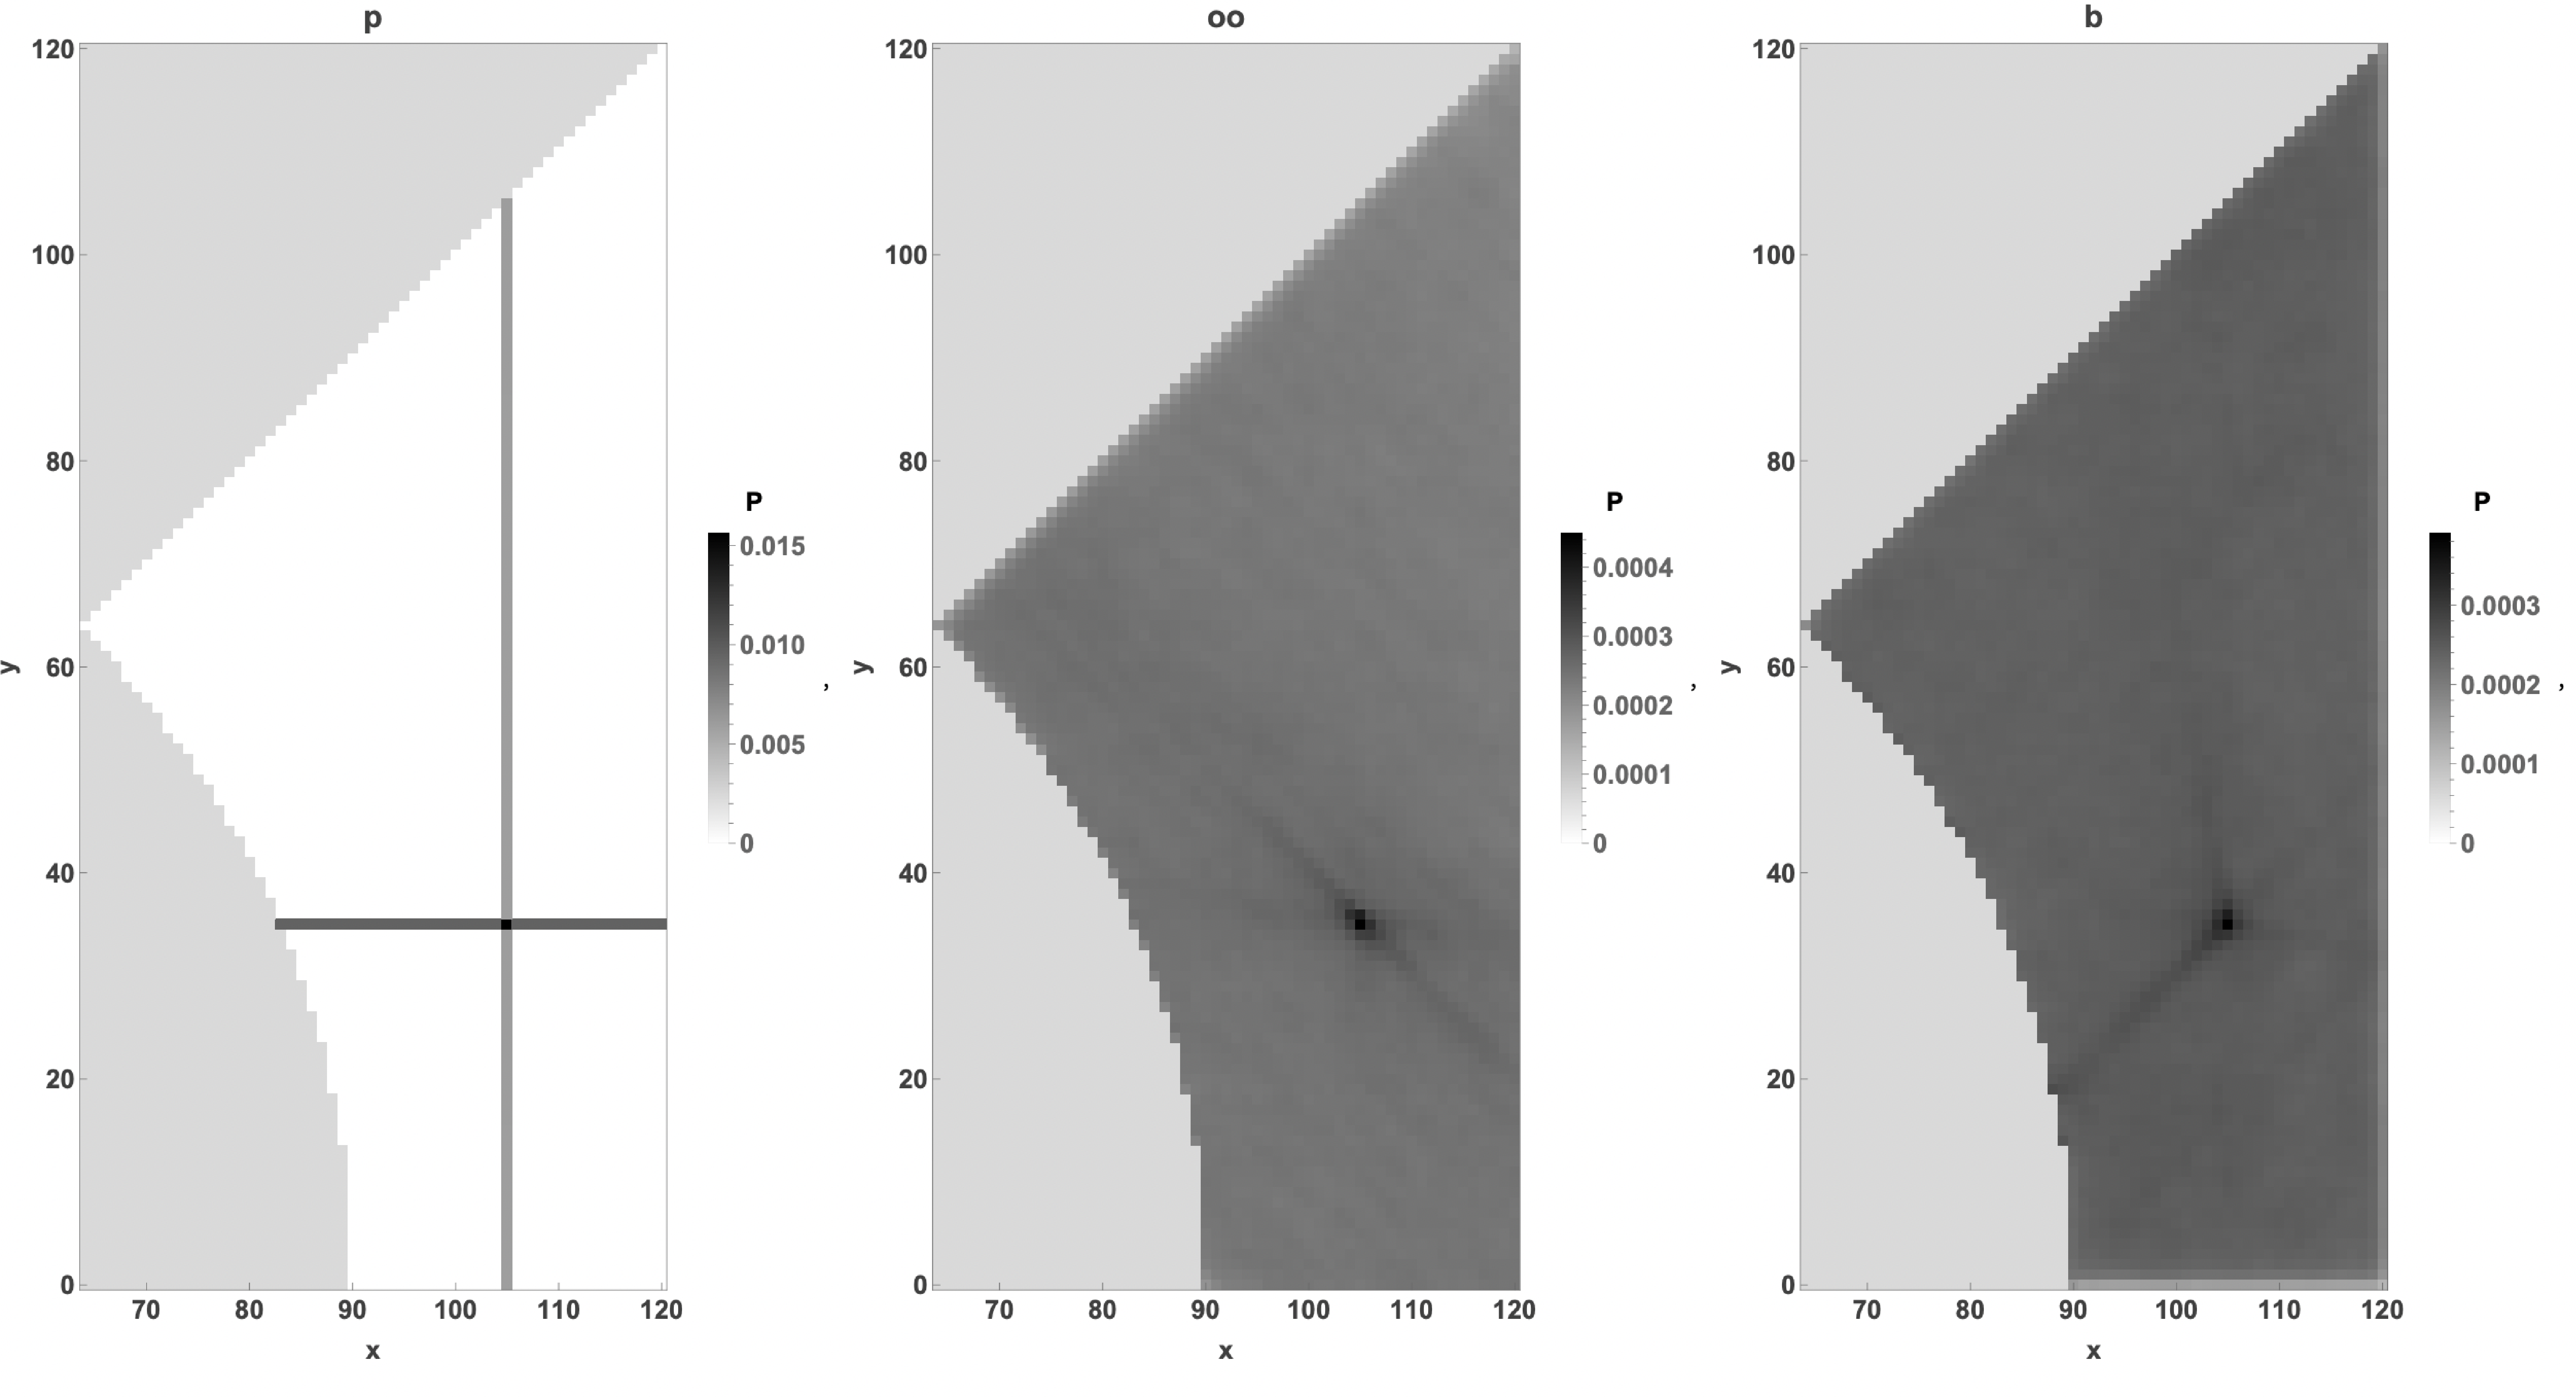
\includegraphics[trim={1060.080bp 0.000bp 1060.080bp 0.000bp},clip,width=\linewidth,height=#1,keepaspectratio]{TimeAverage_Sinai_p-b.pdf}}
\expandafter\def\csname TimeSinaiuoou\endcsname#1{%
  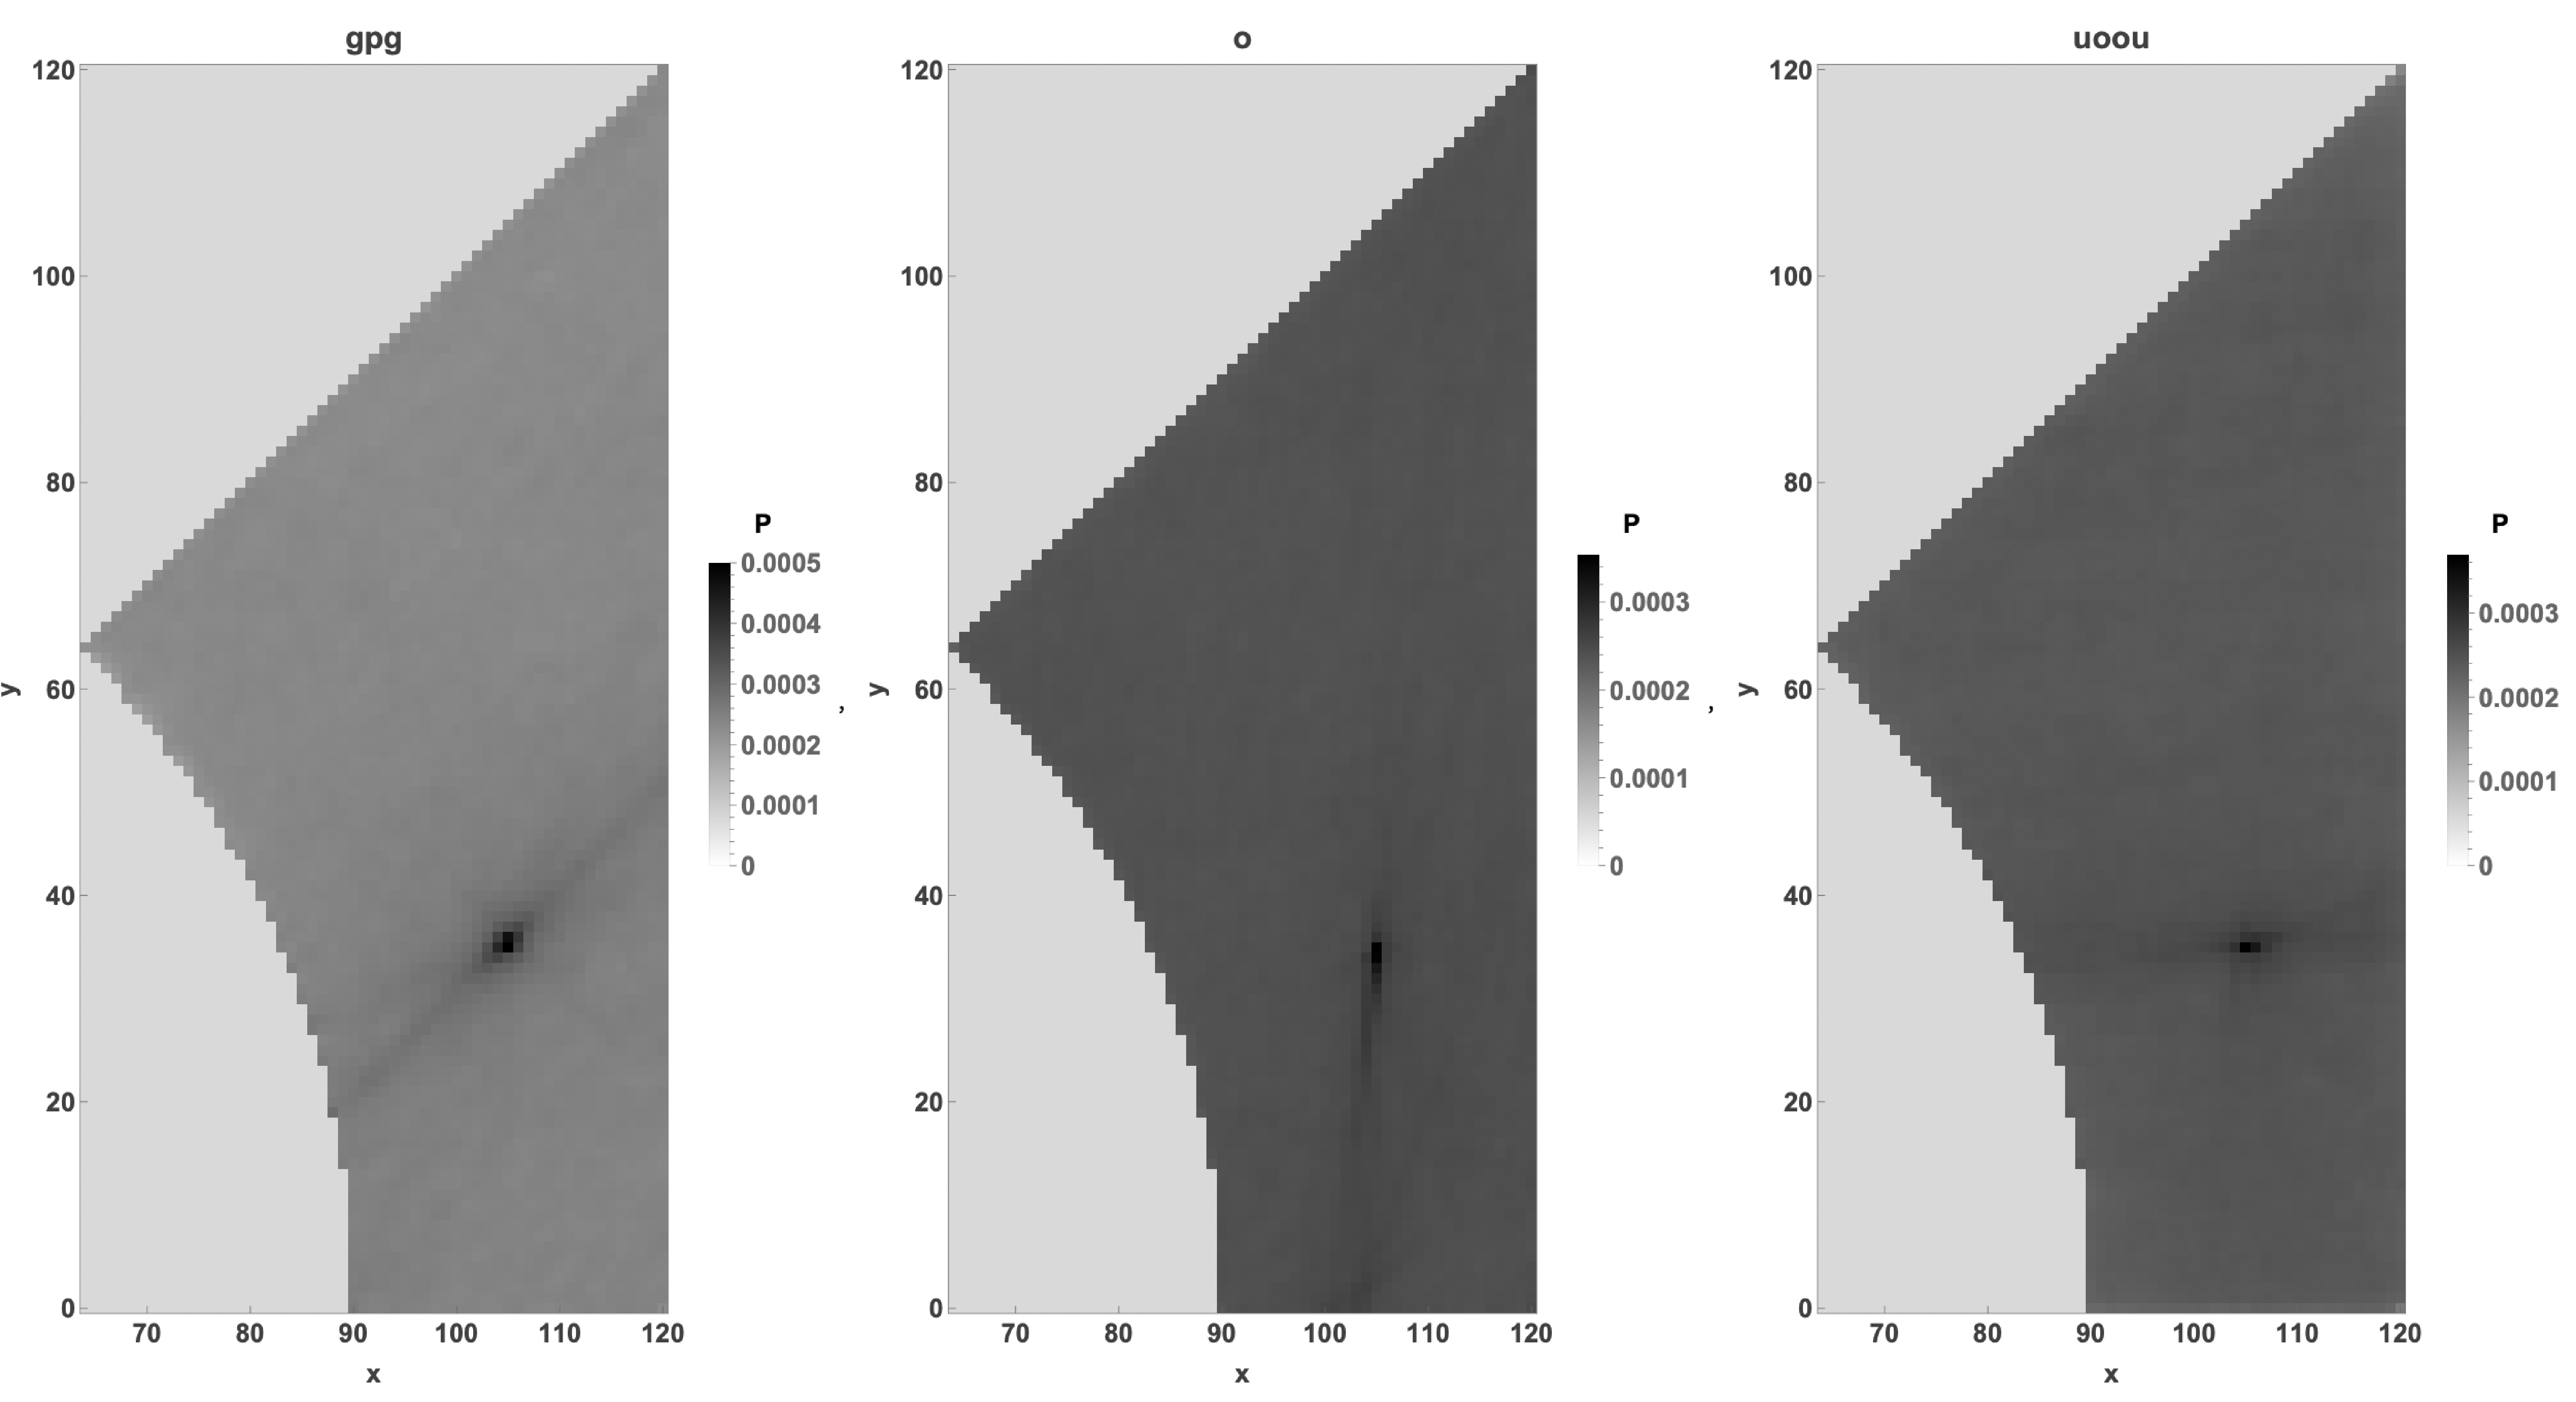
\includegraphics[trim={2116.773bp 0.000bp 0.000bp 0.000bp},clip,width=\linewidth,height=#1,keepaspectratio]{TimeAverage_Sinai_gpg-uoou.pdf}}
\expandafter\def\csname TimeSinaio\endcsname#1{%
  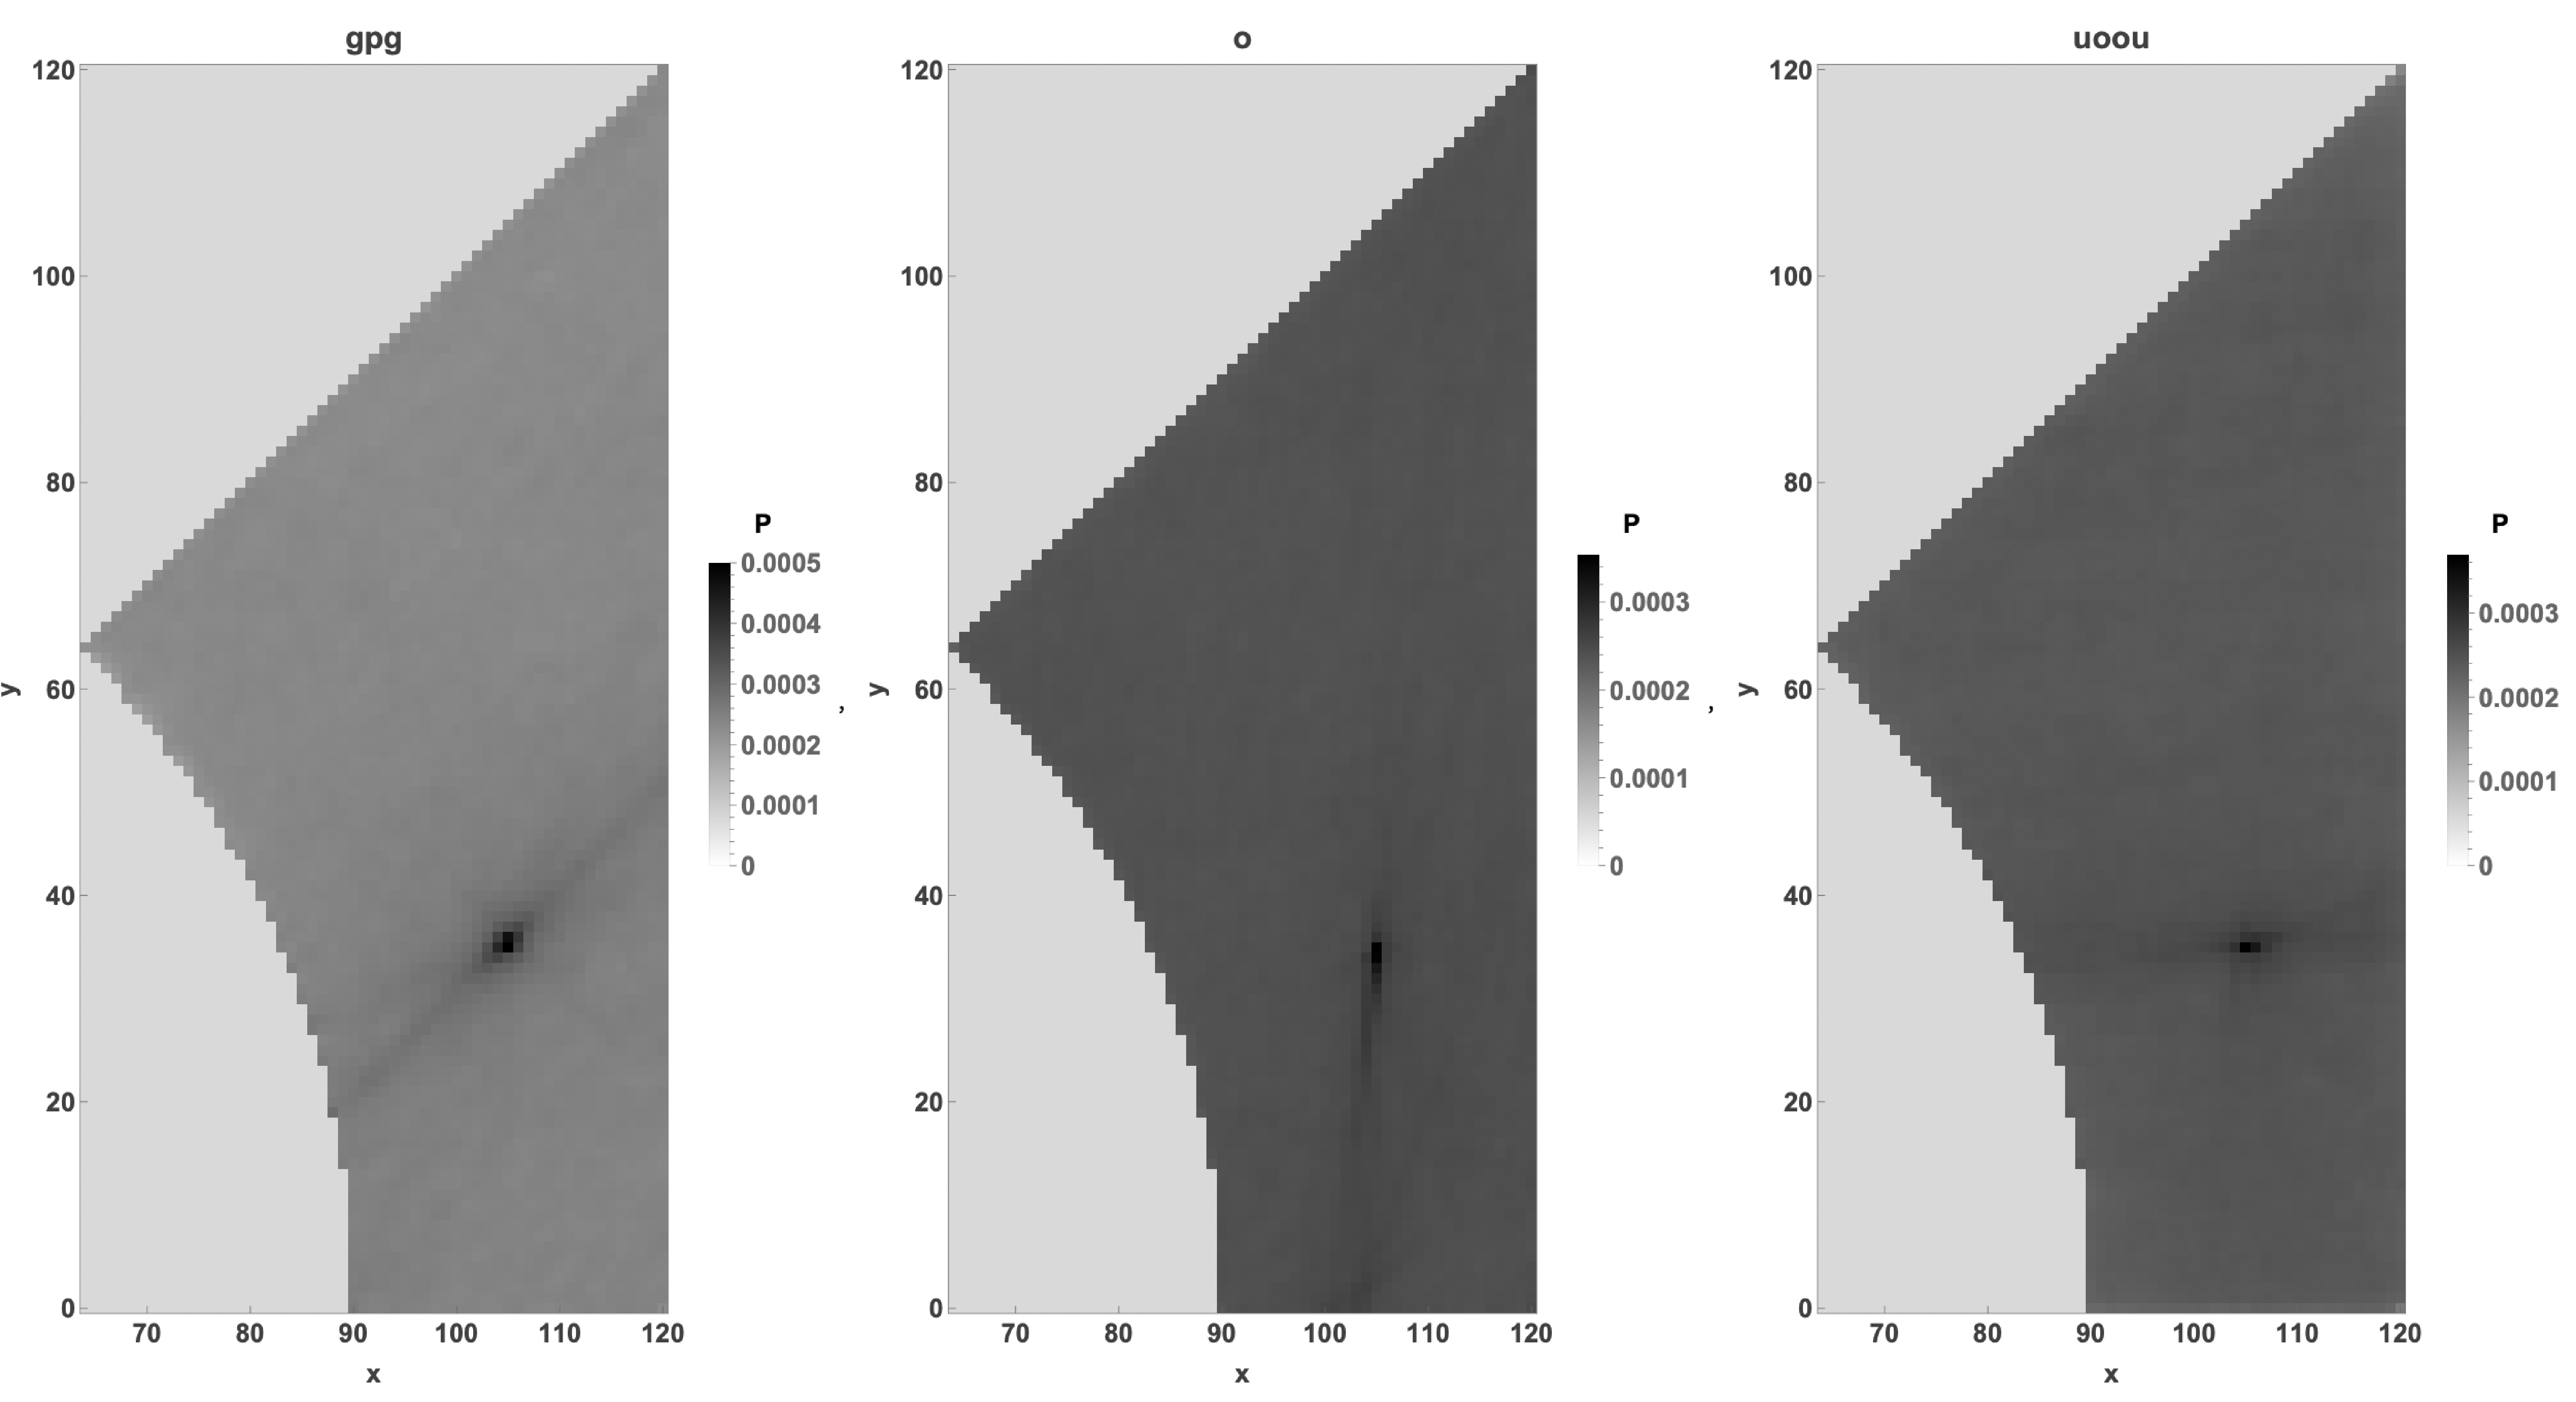
\includegraphics[trim={1058.387bp 0.000bp 1058.387bp 0.000bp},clip,width=\linewidth,height=#1,keepaspectratio]{TimeAverage_Sinai_gpg-uoou.pdf}}
\expandafter\def\csname TimeSinaib\endcsname#1{%
  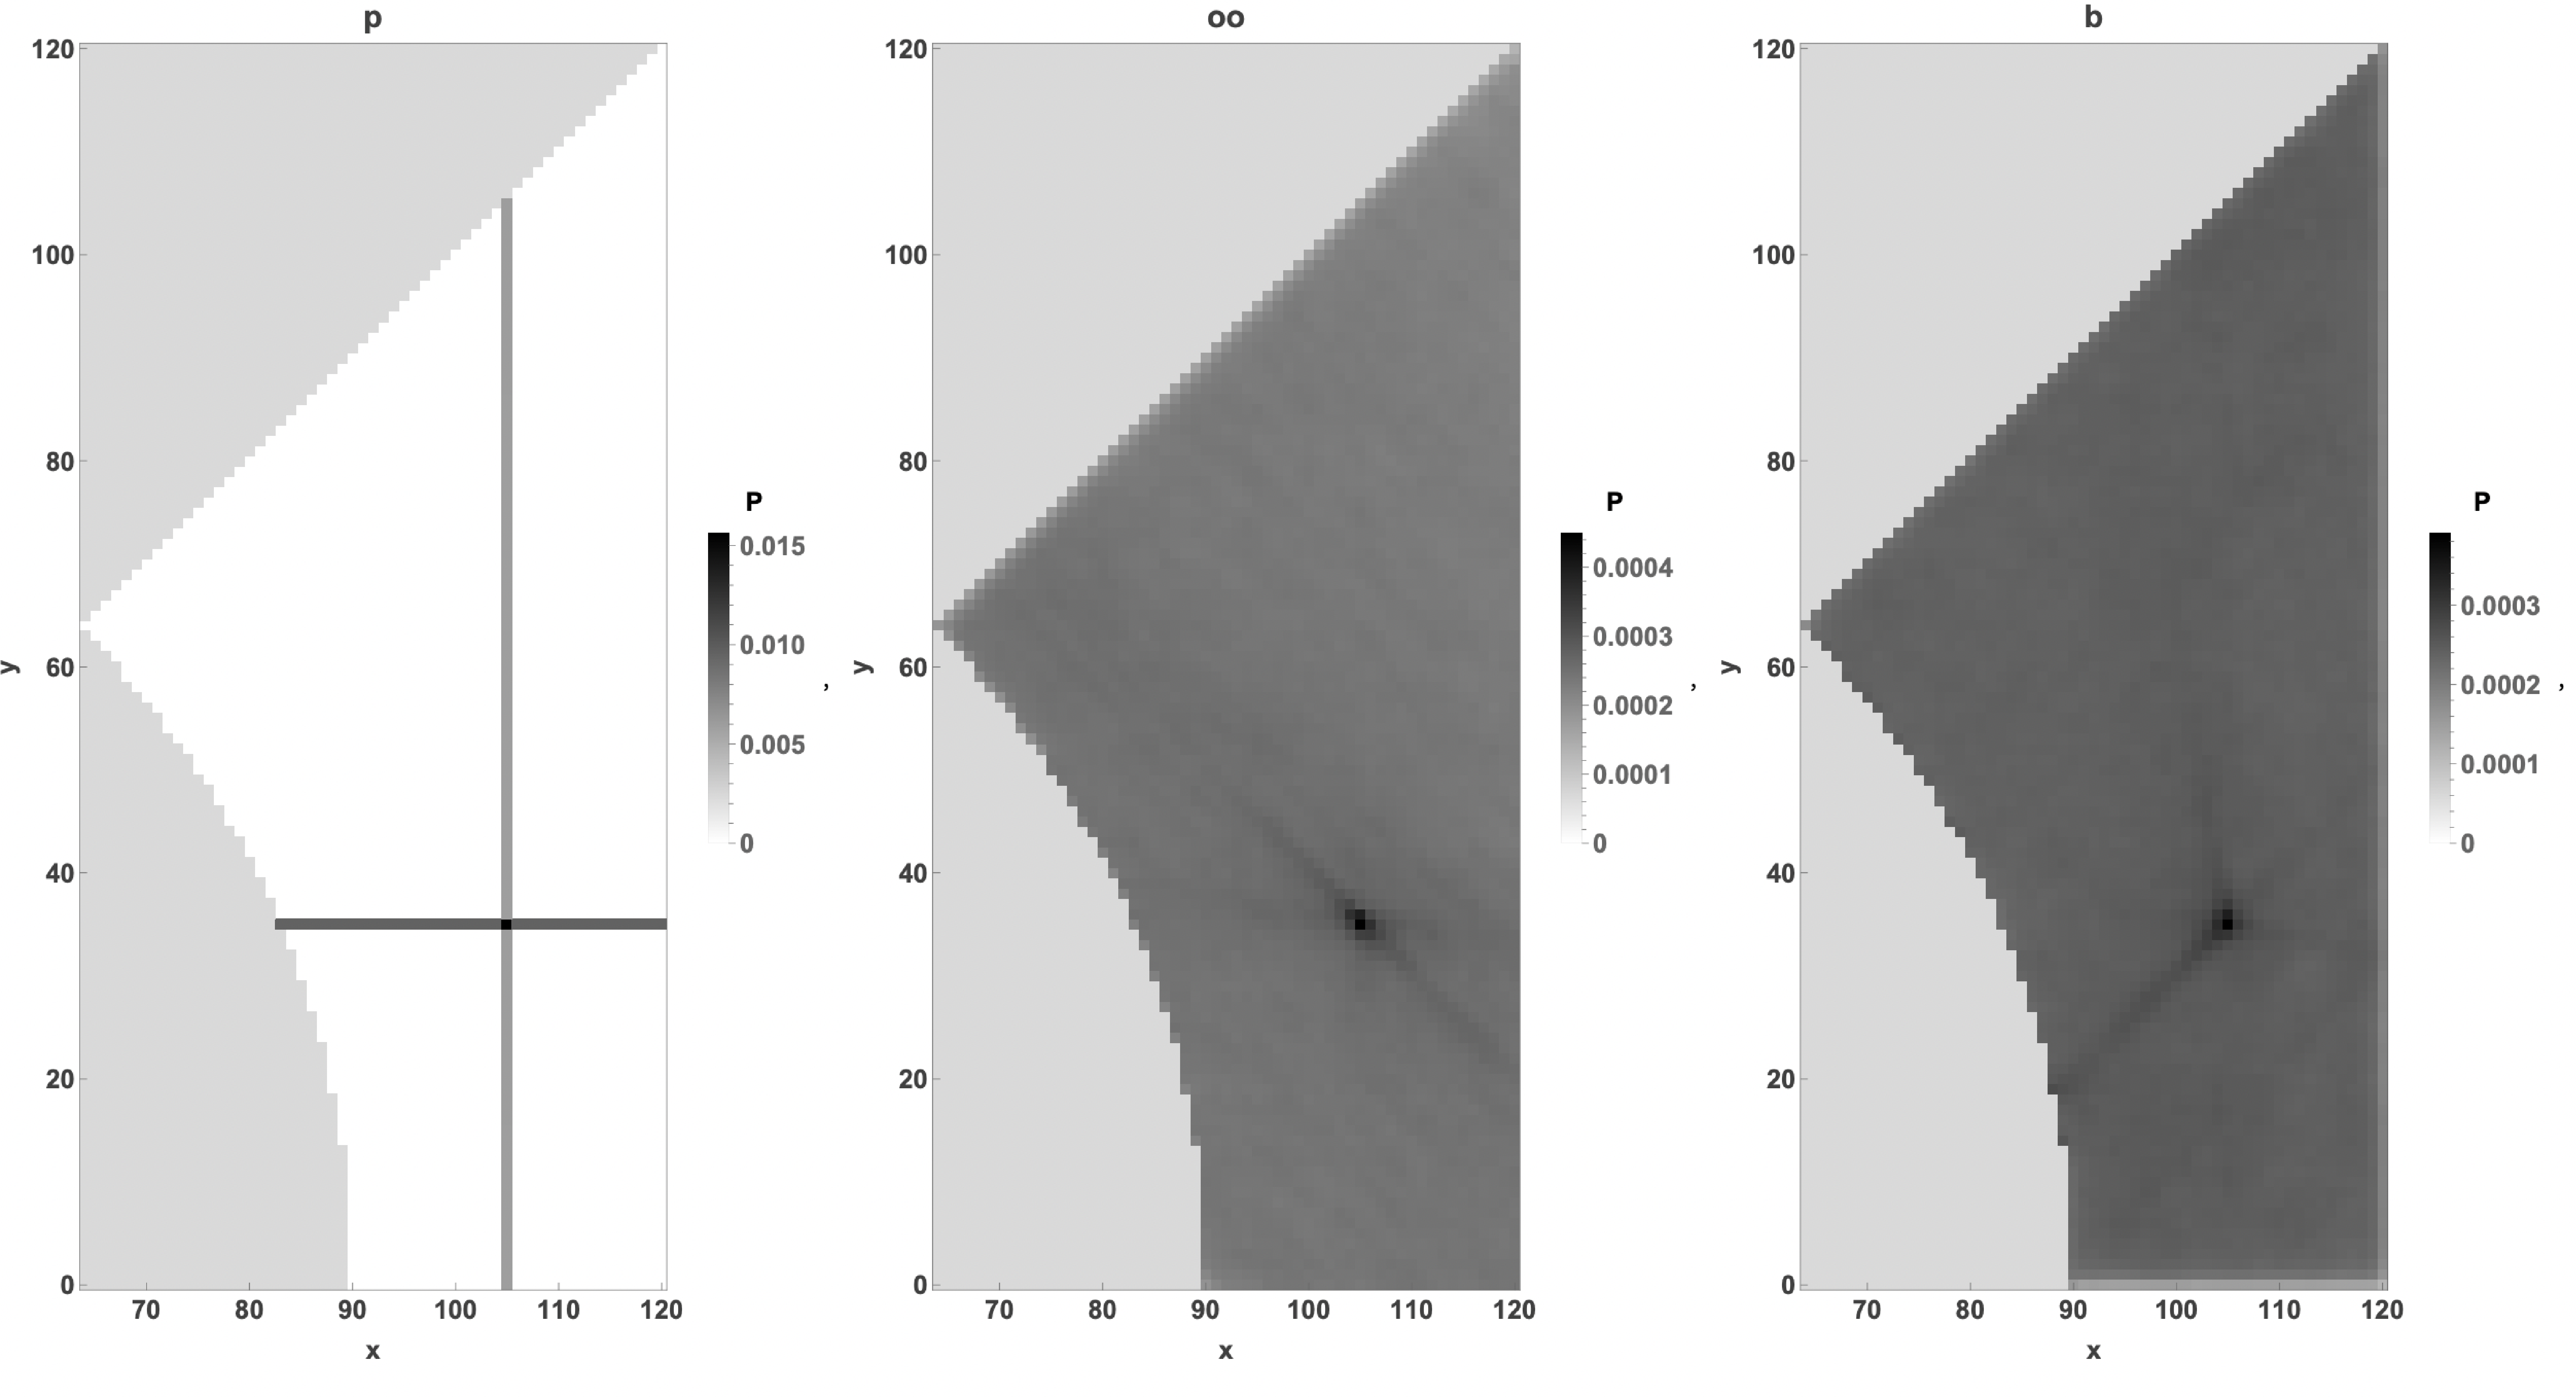
\includegraphics[trim={2120.160bp 0.000bp 0.000bp 0.000bp},clip,width=\linewidth,height=#1,keepaspectratio]{TimeAverage_Sinai_p-b.pdf}}
\expandafter\def\csname TimeSinaiubu\endcsname#1{%
  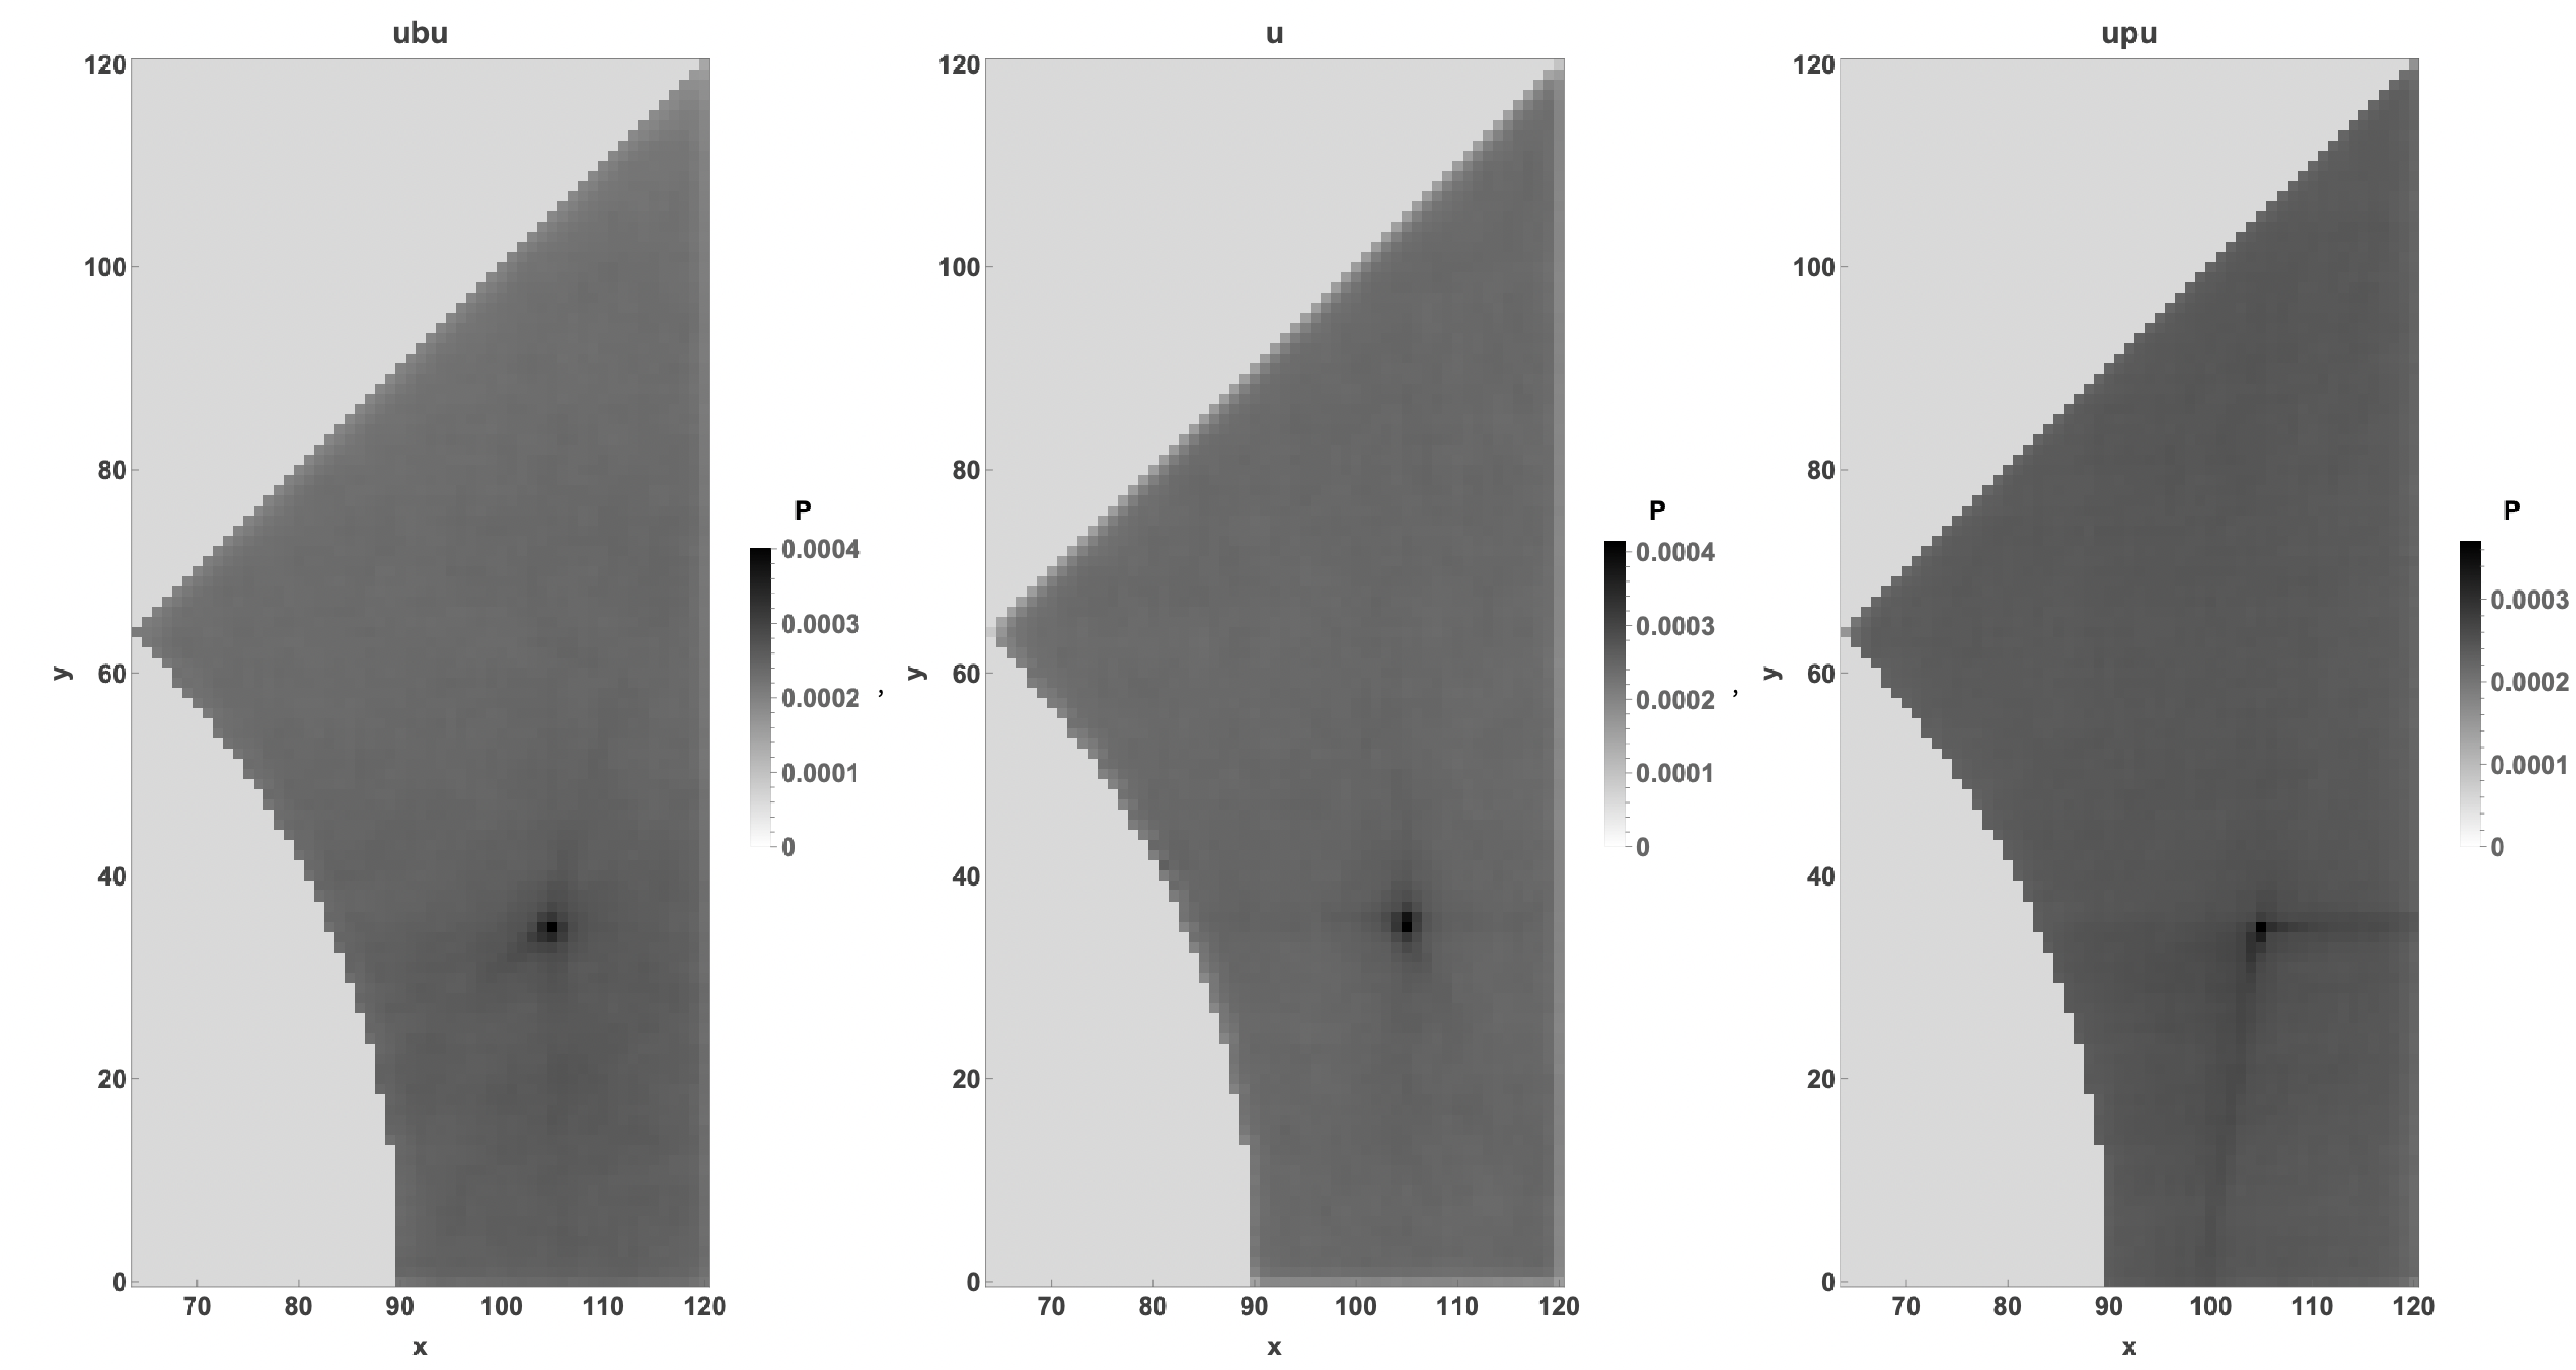
\includegraphics[trim={0.000bp 0.000bp 2152.340bp 0.000bp},clip,width=\linewidth,height=#1,keepaspectratio]{TimeAverage_Sinai_ubu-upu.pdf}}
\expandafter\def\csname TimeSinaiu\endcsname#1{%
  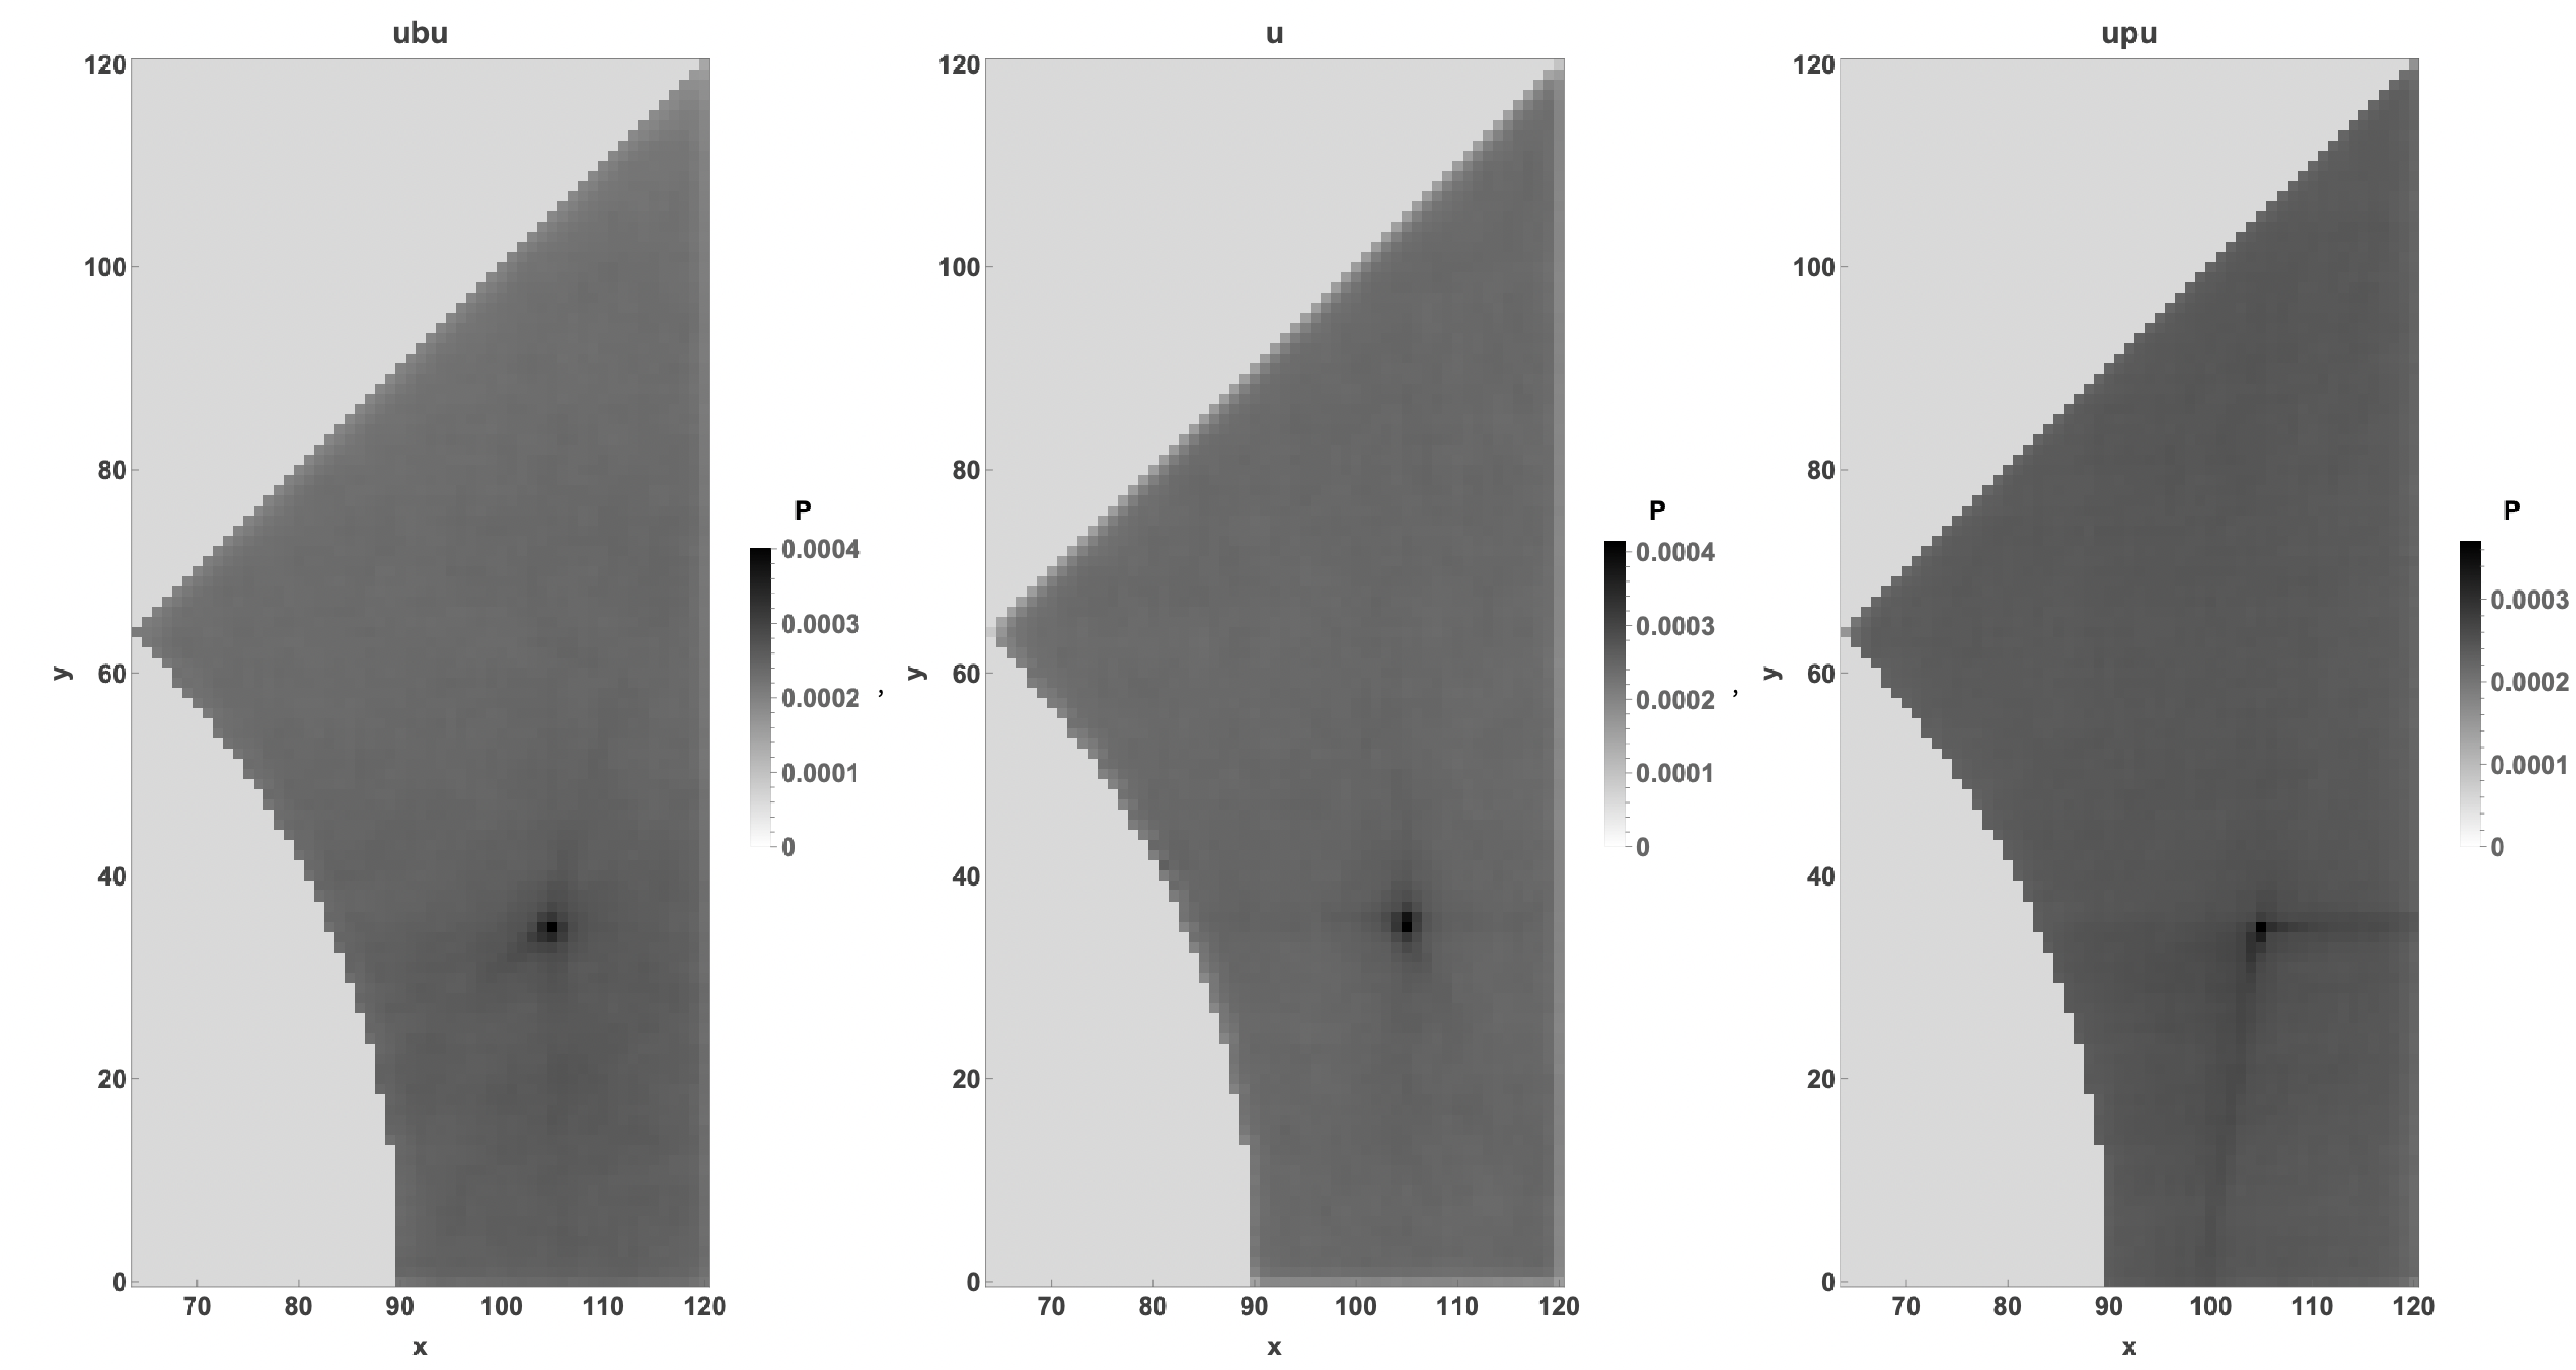
\includegraphics[trim={1076.170bp 0.000bp 1076.170bp 0.000bp},clip,width=\linewidth,height=#1,keepaspectratio]{TimeAverage_Sinai_ubu-upu.pdf}}
\expandafter\def\csname TimeSinaiupu\endcsname#1{%
  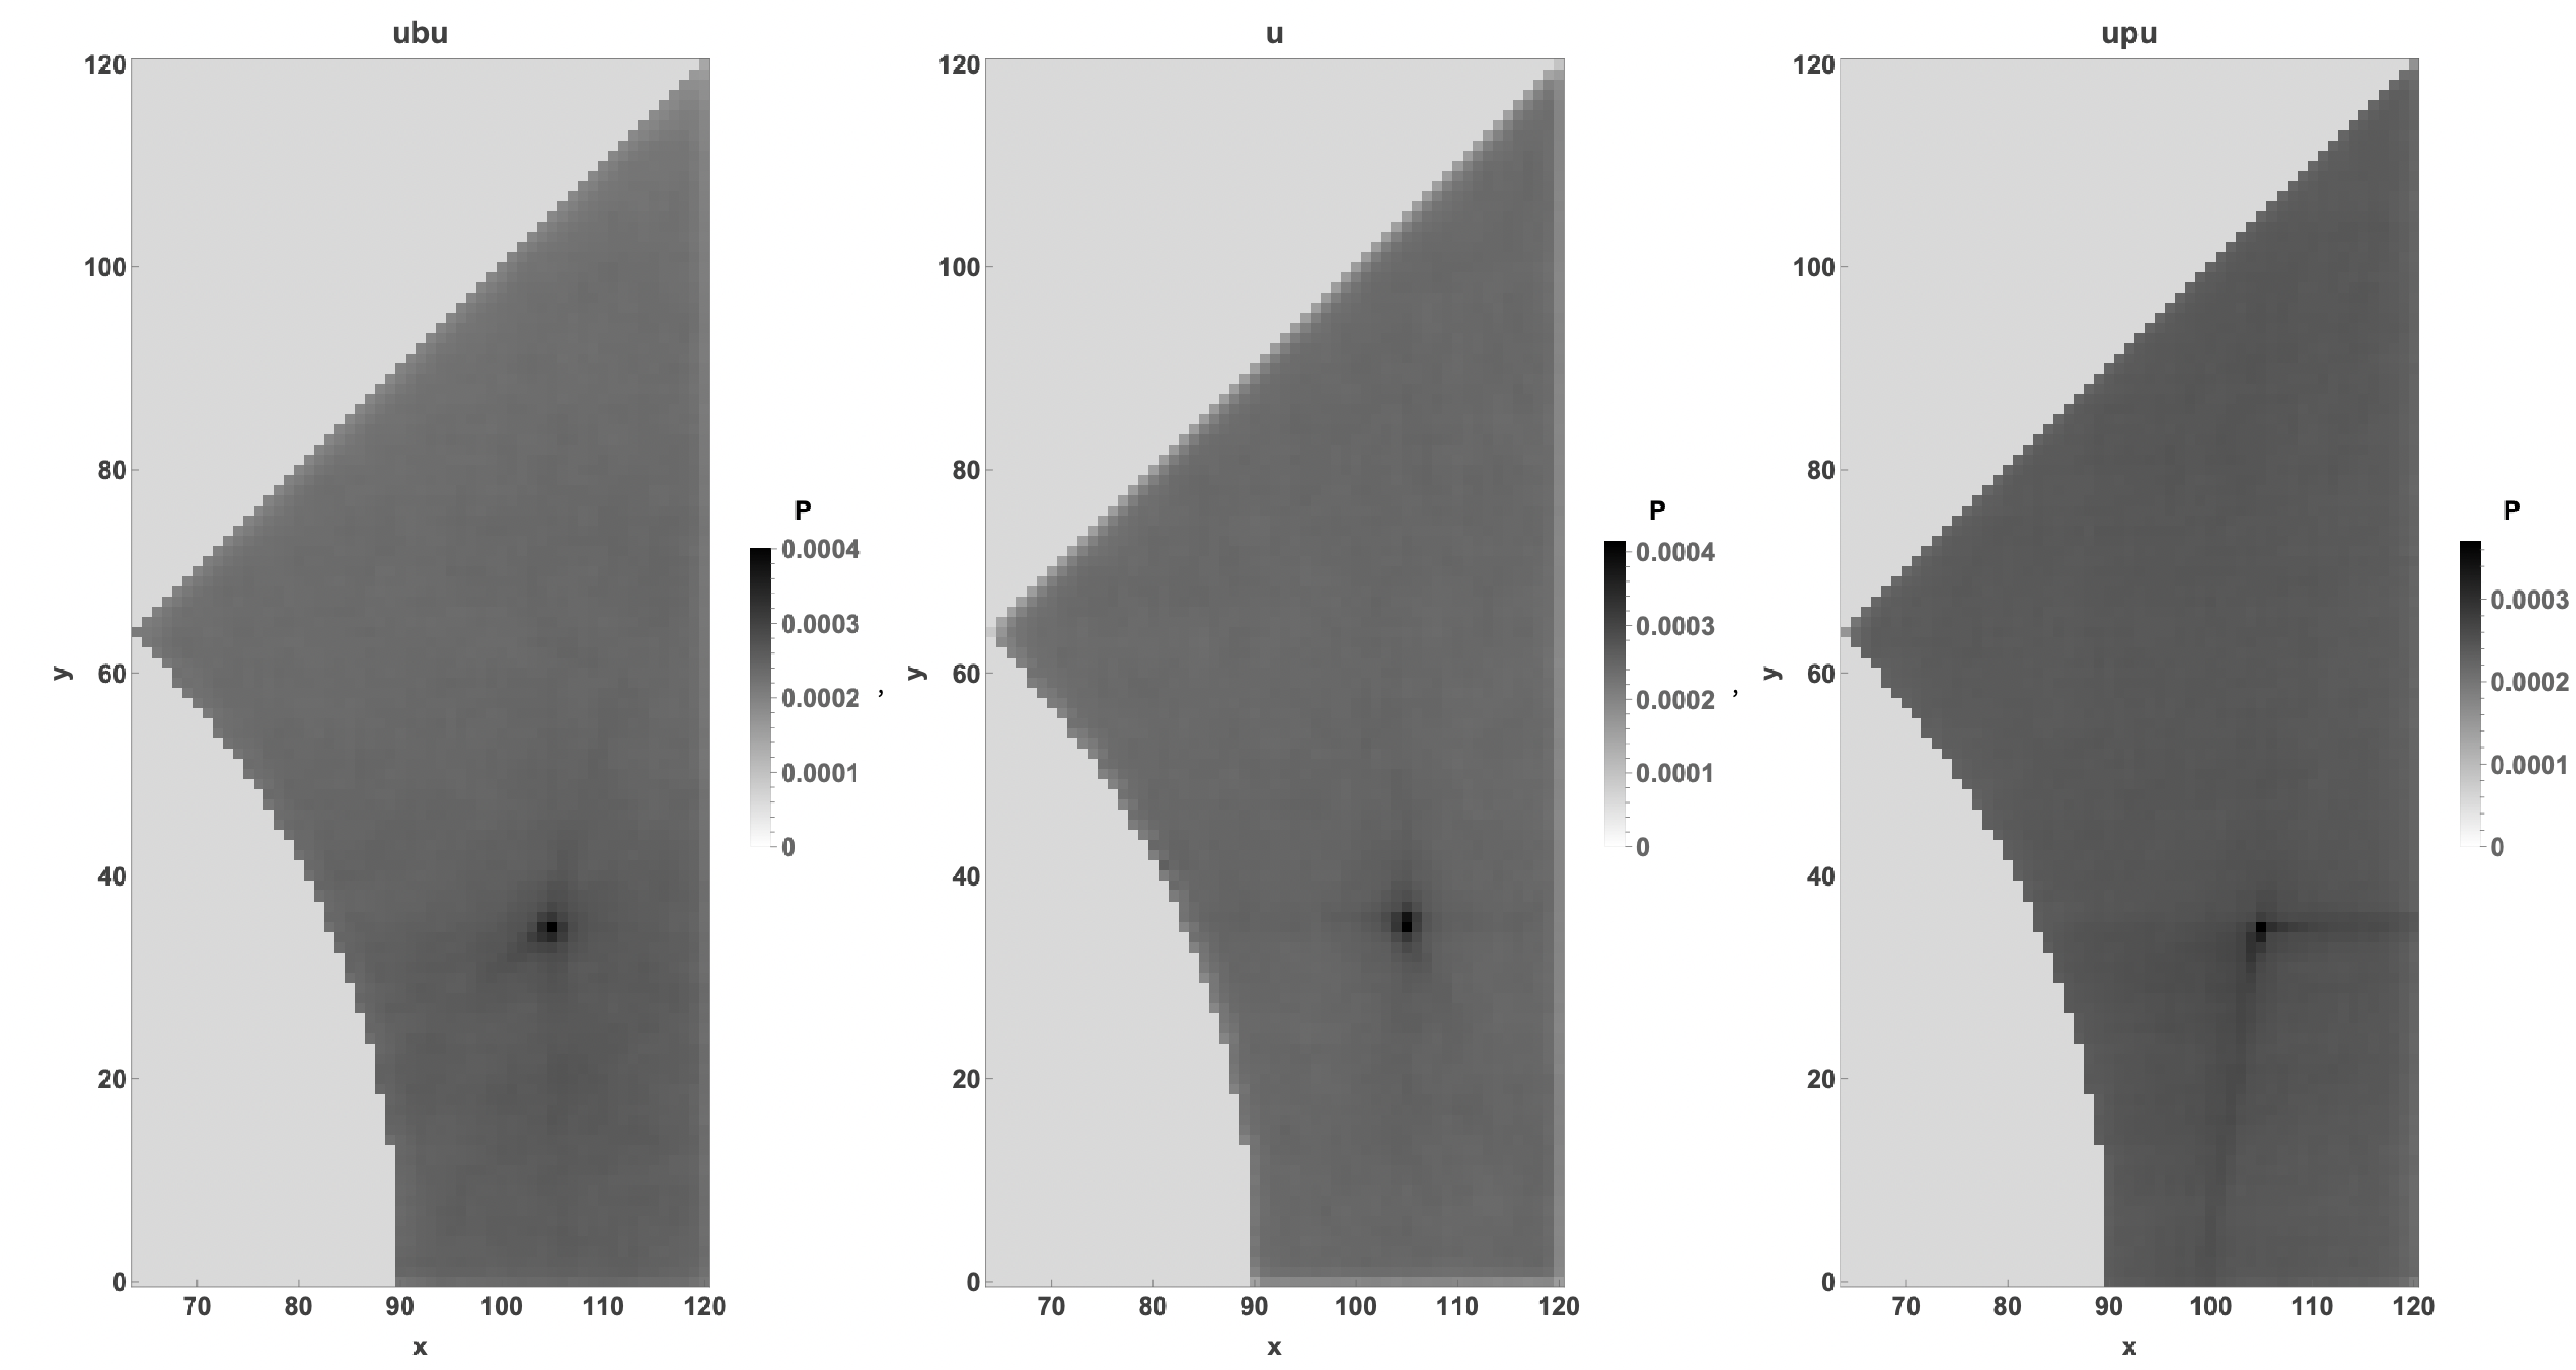
\includegraphics[trim={2152.340bp 0.000bp 0.000bp 0.000bp},clip,width=\linewidth,height=#1,keepaspectratio]{TimeAverage_Sinai_ubu-upu.pdf}}
\expandafter\def\csname TimeSinaip\endcsname#1{%
  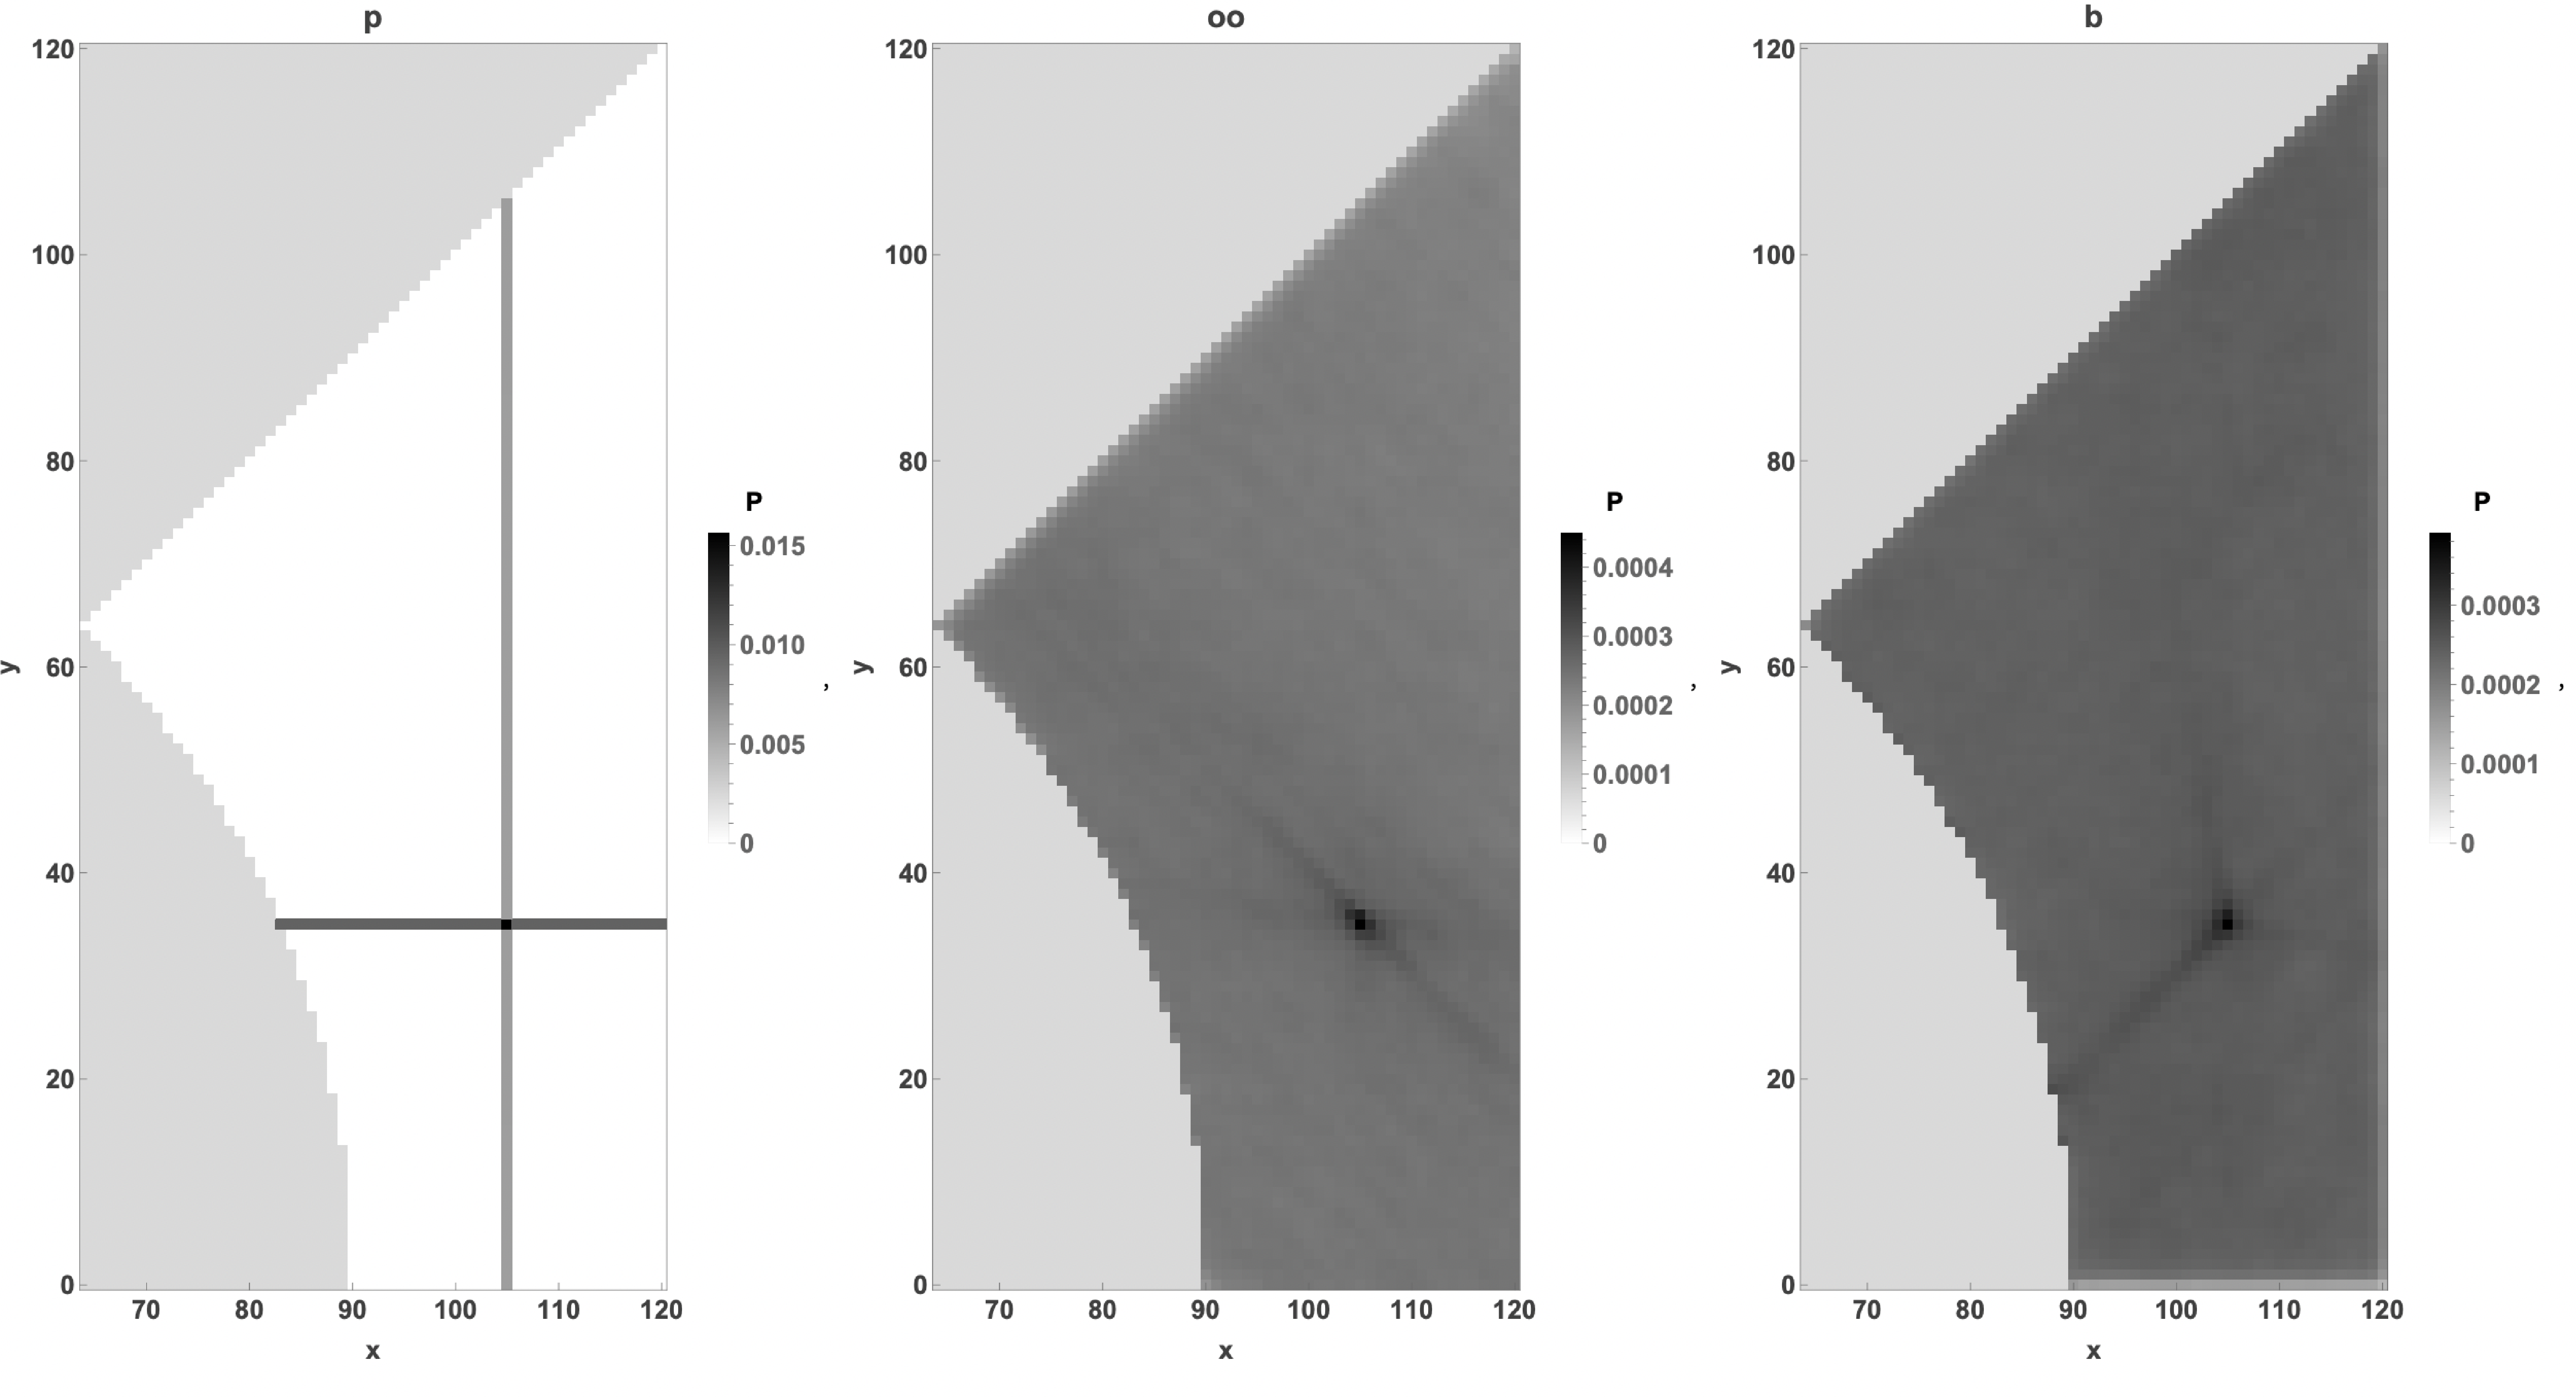
\includegraphics[trim={0.000bp 0.000bp 2120.160bp 0.000bp},clip,width=\linewidth,height=#1,keepaspectratio]{TimeAverage_Sinai_p-b.pdf}}
\expandafter\def\csname DensityRectFour\endcsname#1{%
  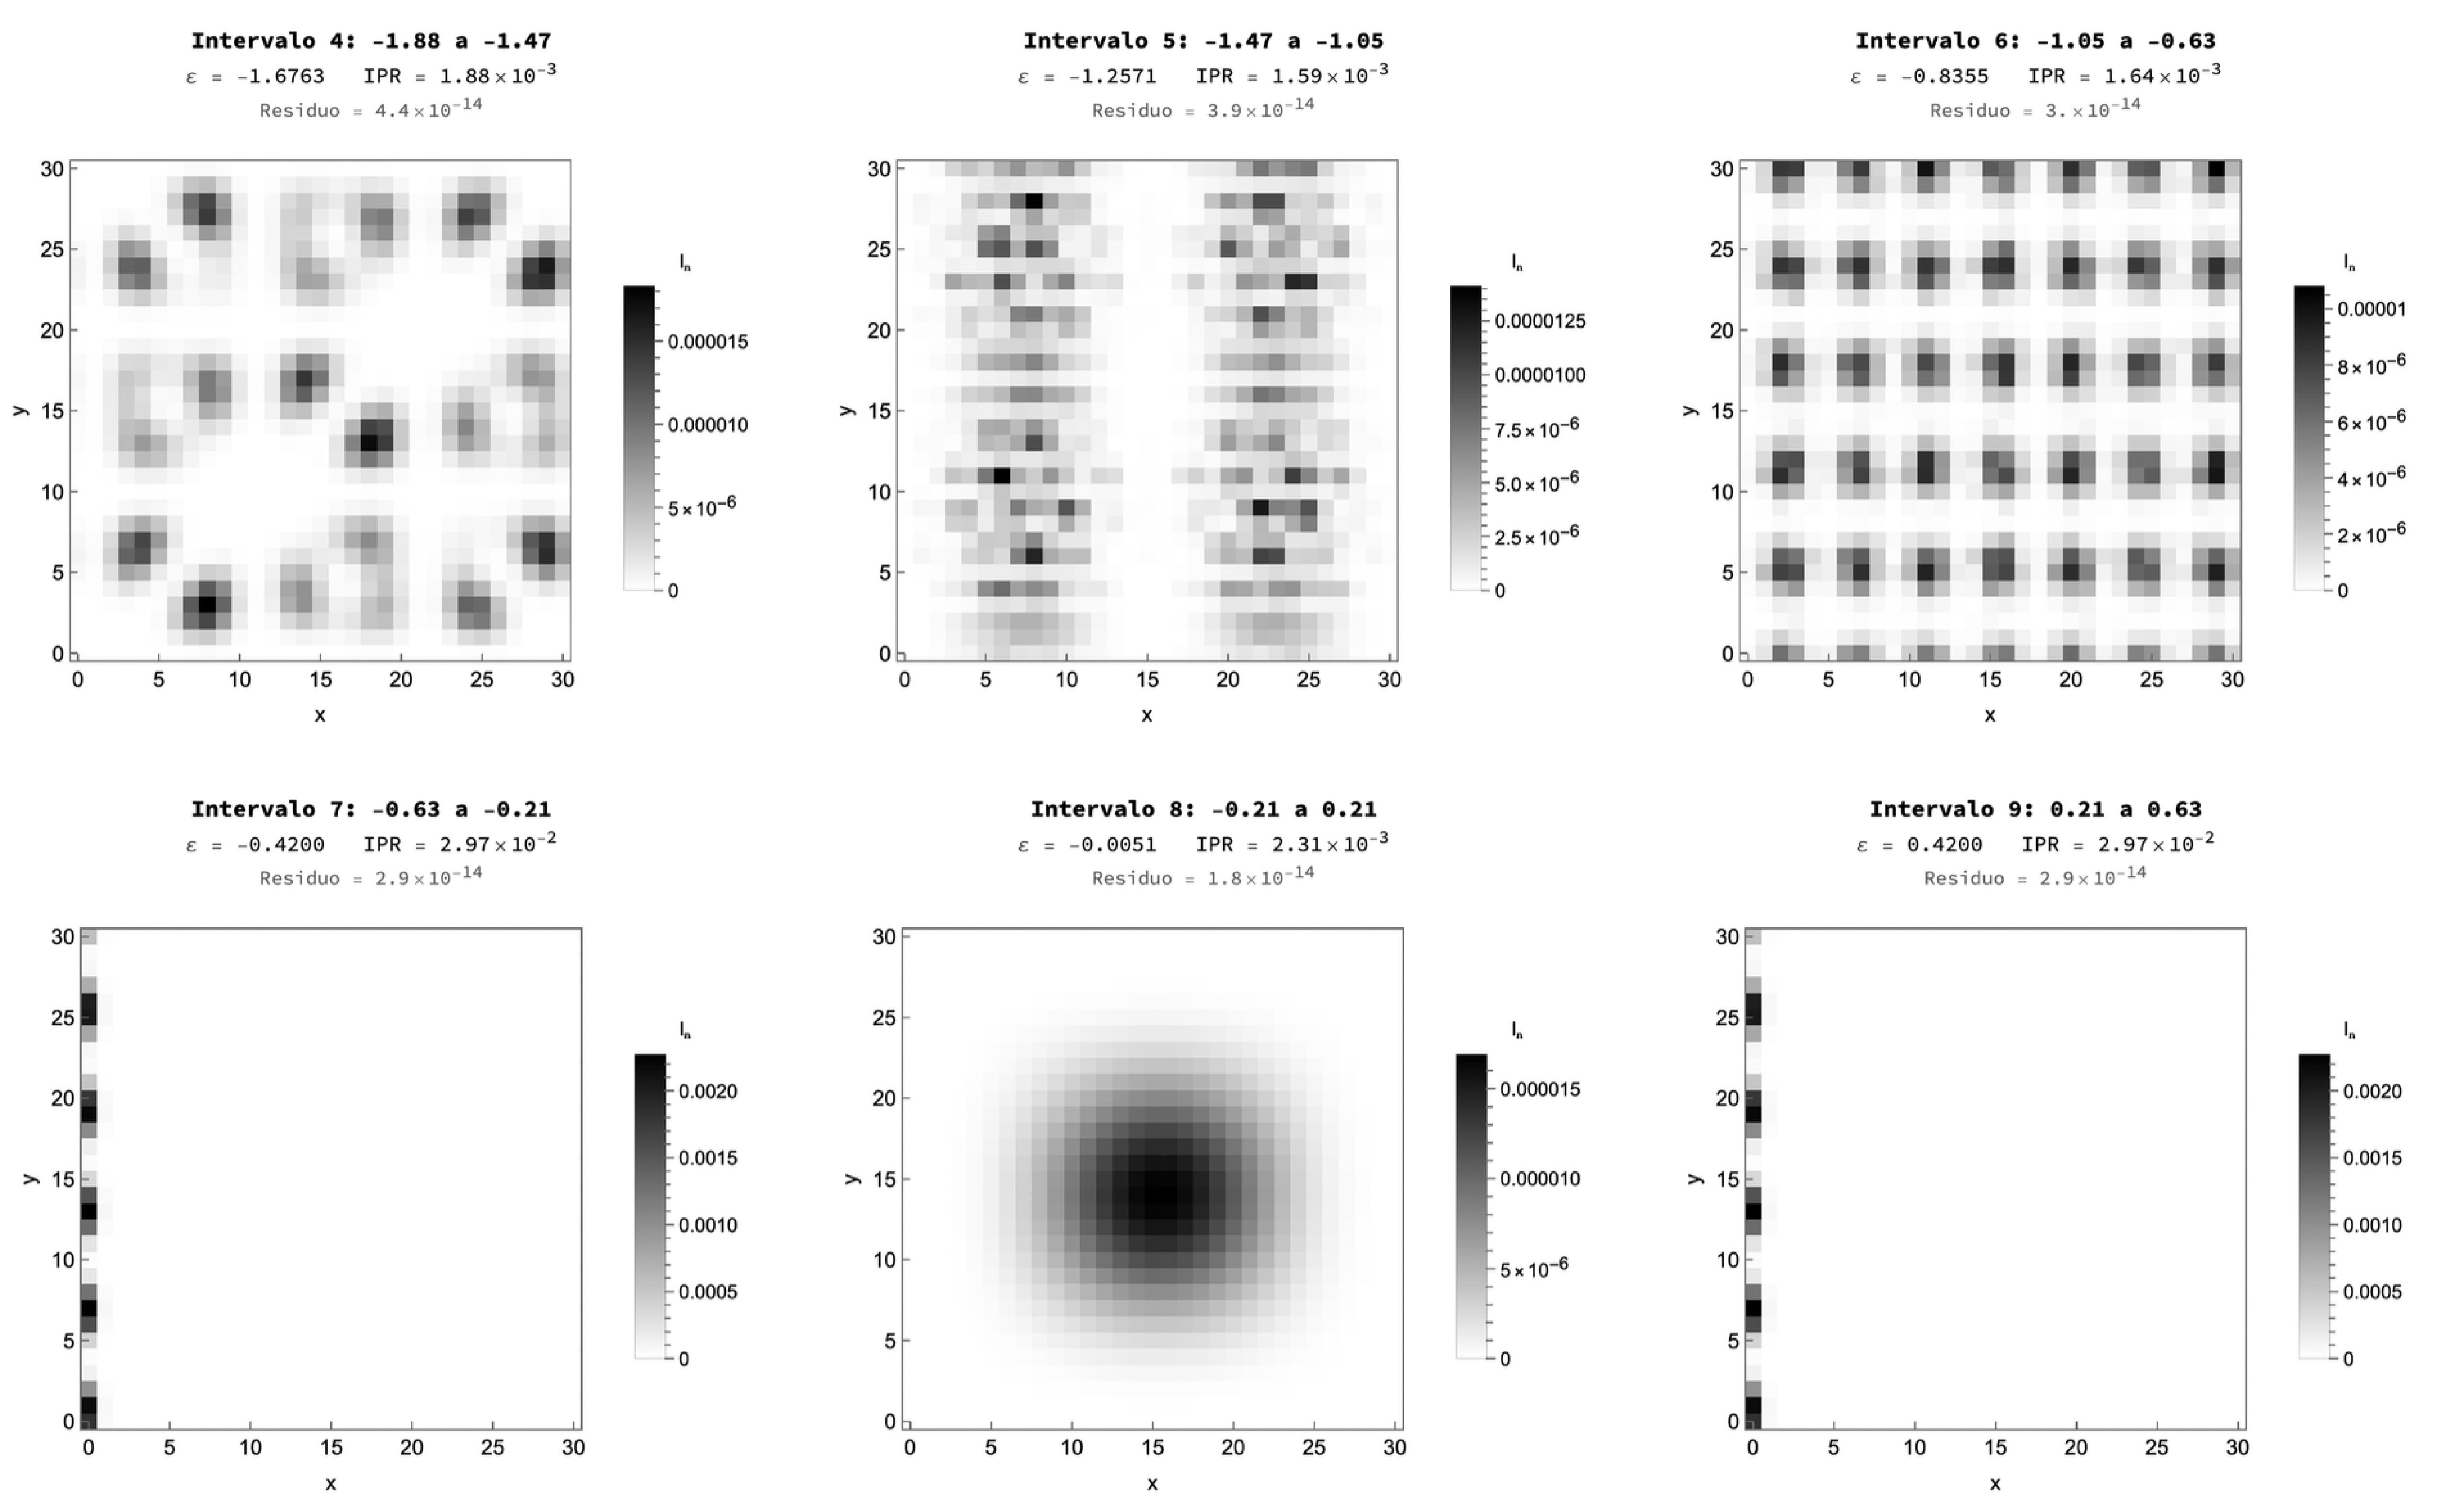
\includegraphics[trim={0.000bp 739.180bp 1623.993bp 0.000bp},clip,width=\linewidth,height=#1,keepaspectratio]{IPRDensity_Rect_Intervals04-09.pdf}}
\expandafter\def\csname DensityRectSeven\endcsname#1{%
  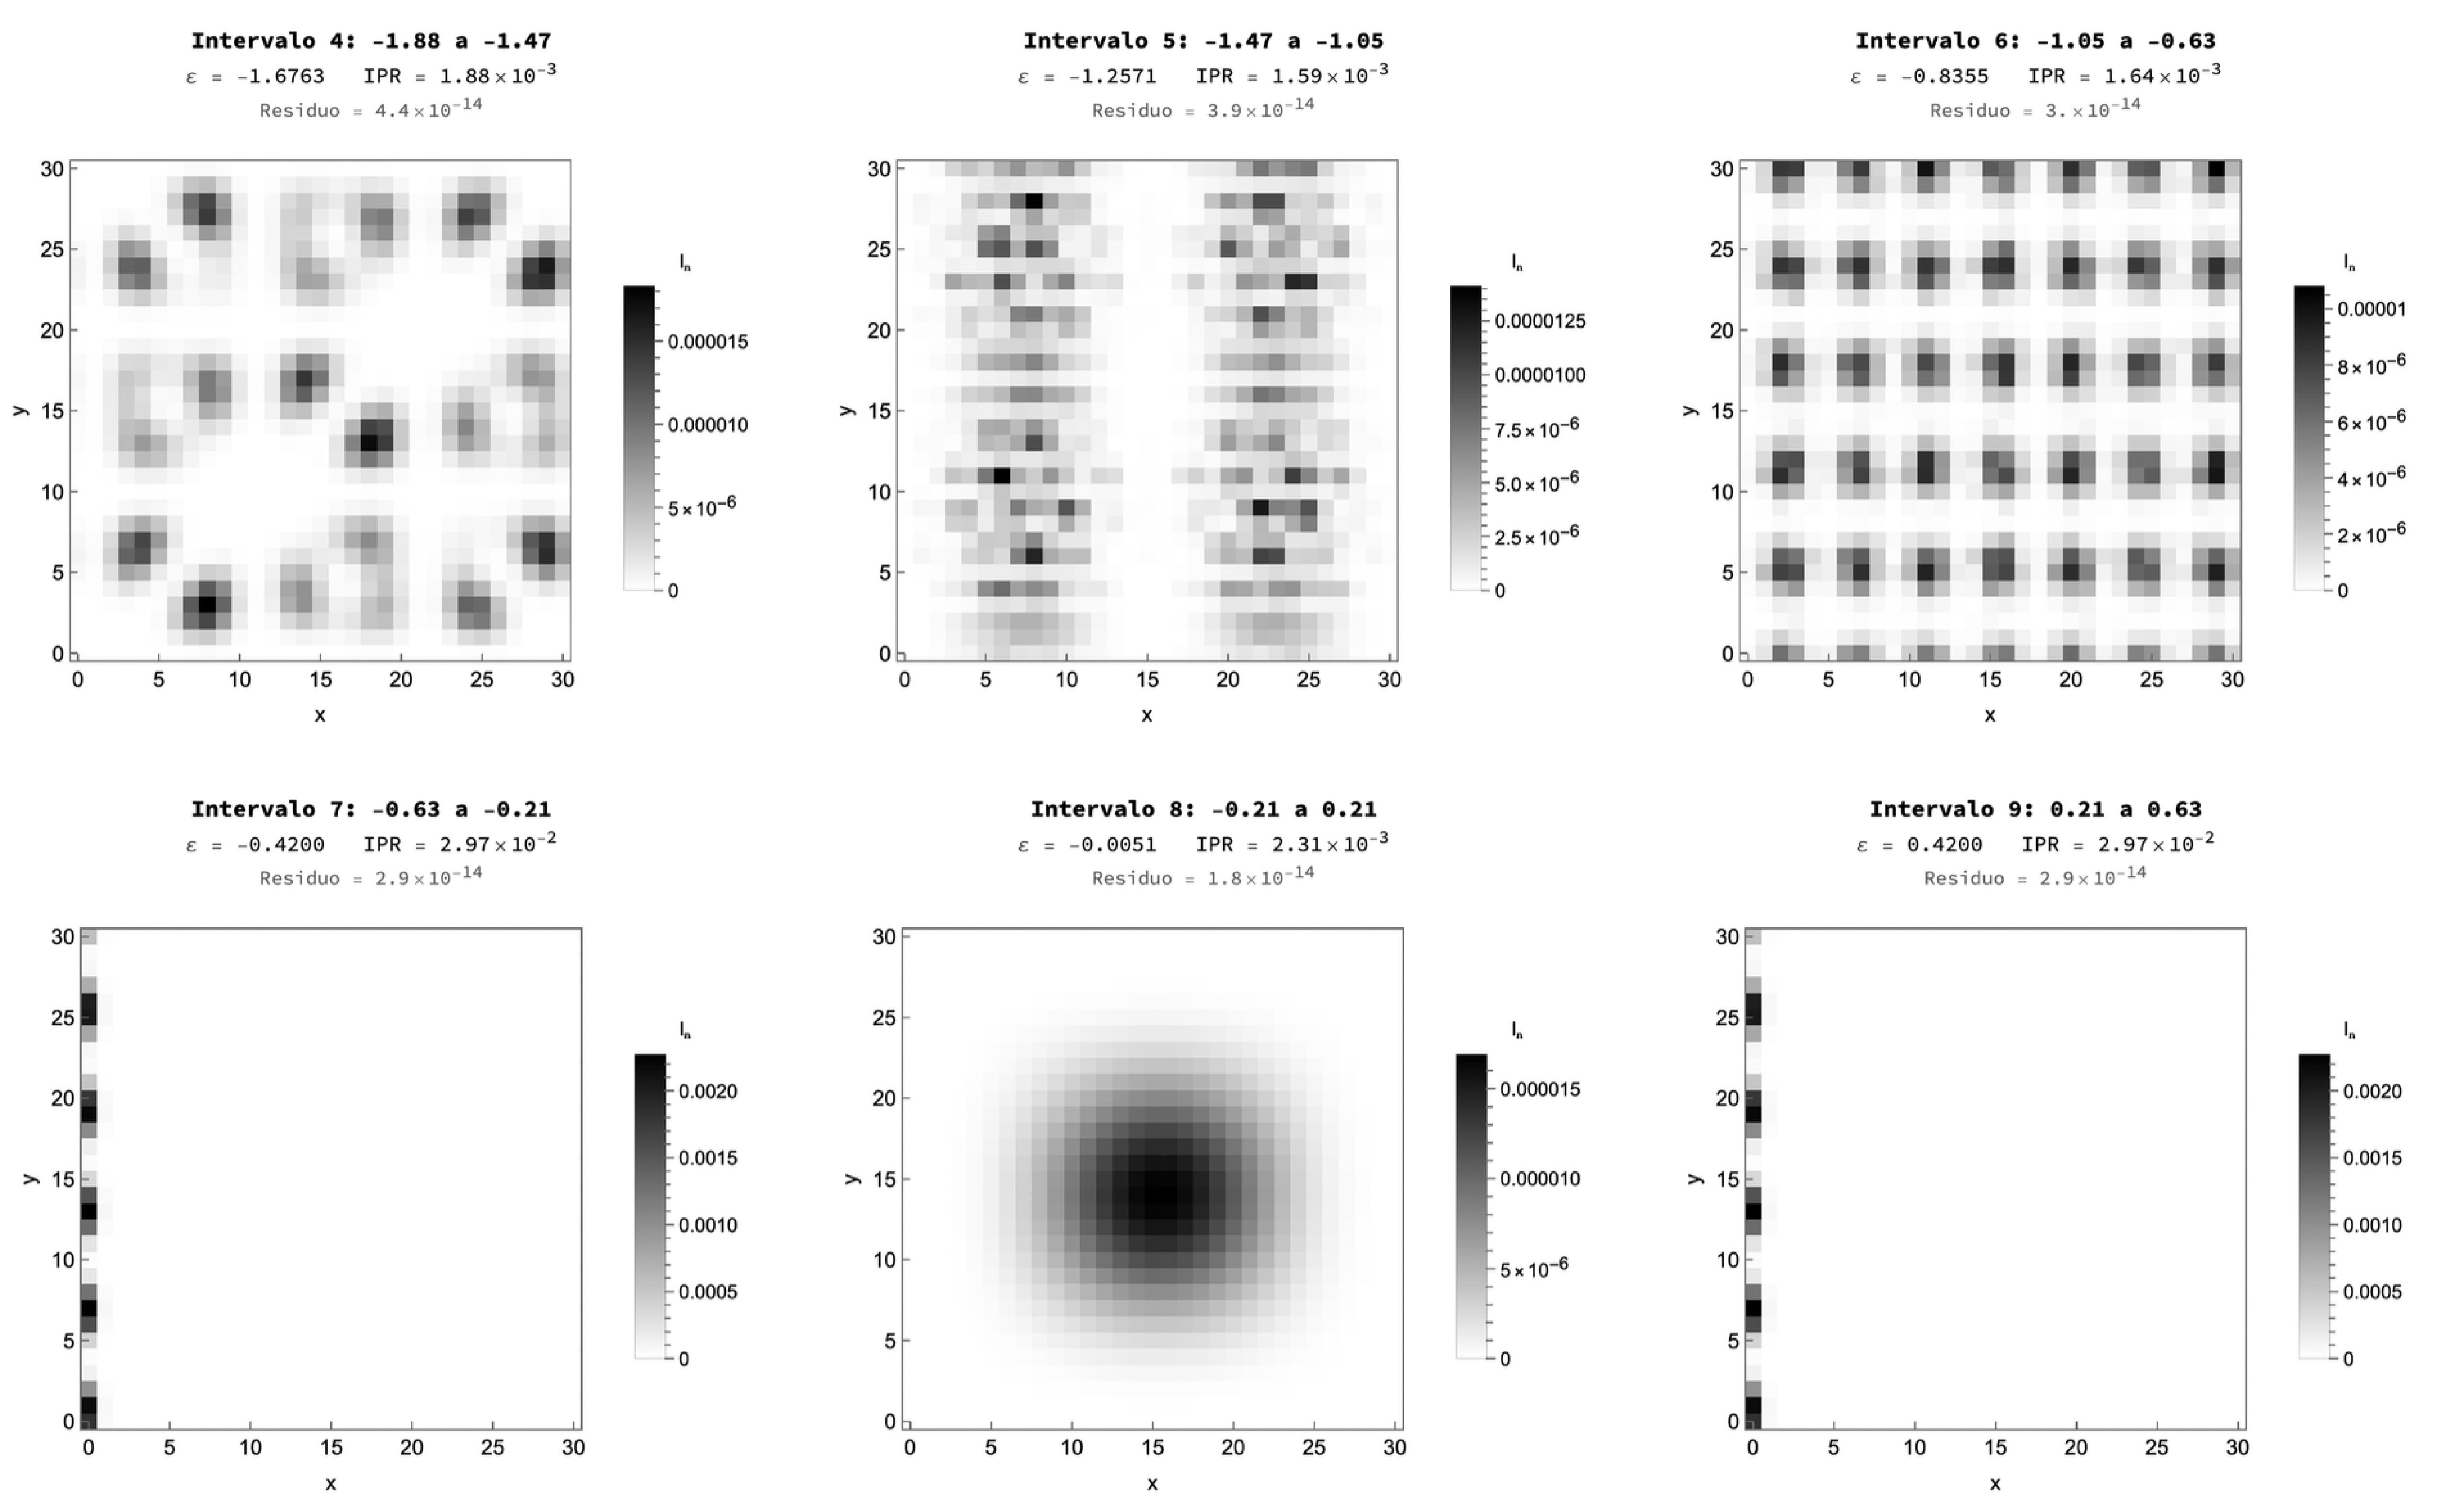
\includegraphics[trim={0.000bp 0.000bp 1623.993bp 739.180bp},clip,width=\linewidth,height=#1,keepaspectratio]{IPRDensity_Rect_Intervals04-09.pdf}}
\expandafter\def\csname DensitySinaiOne\endcsname#1{%
  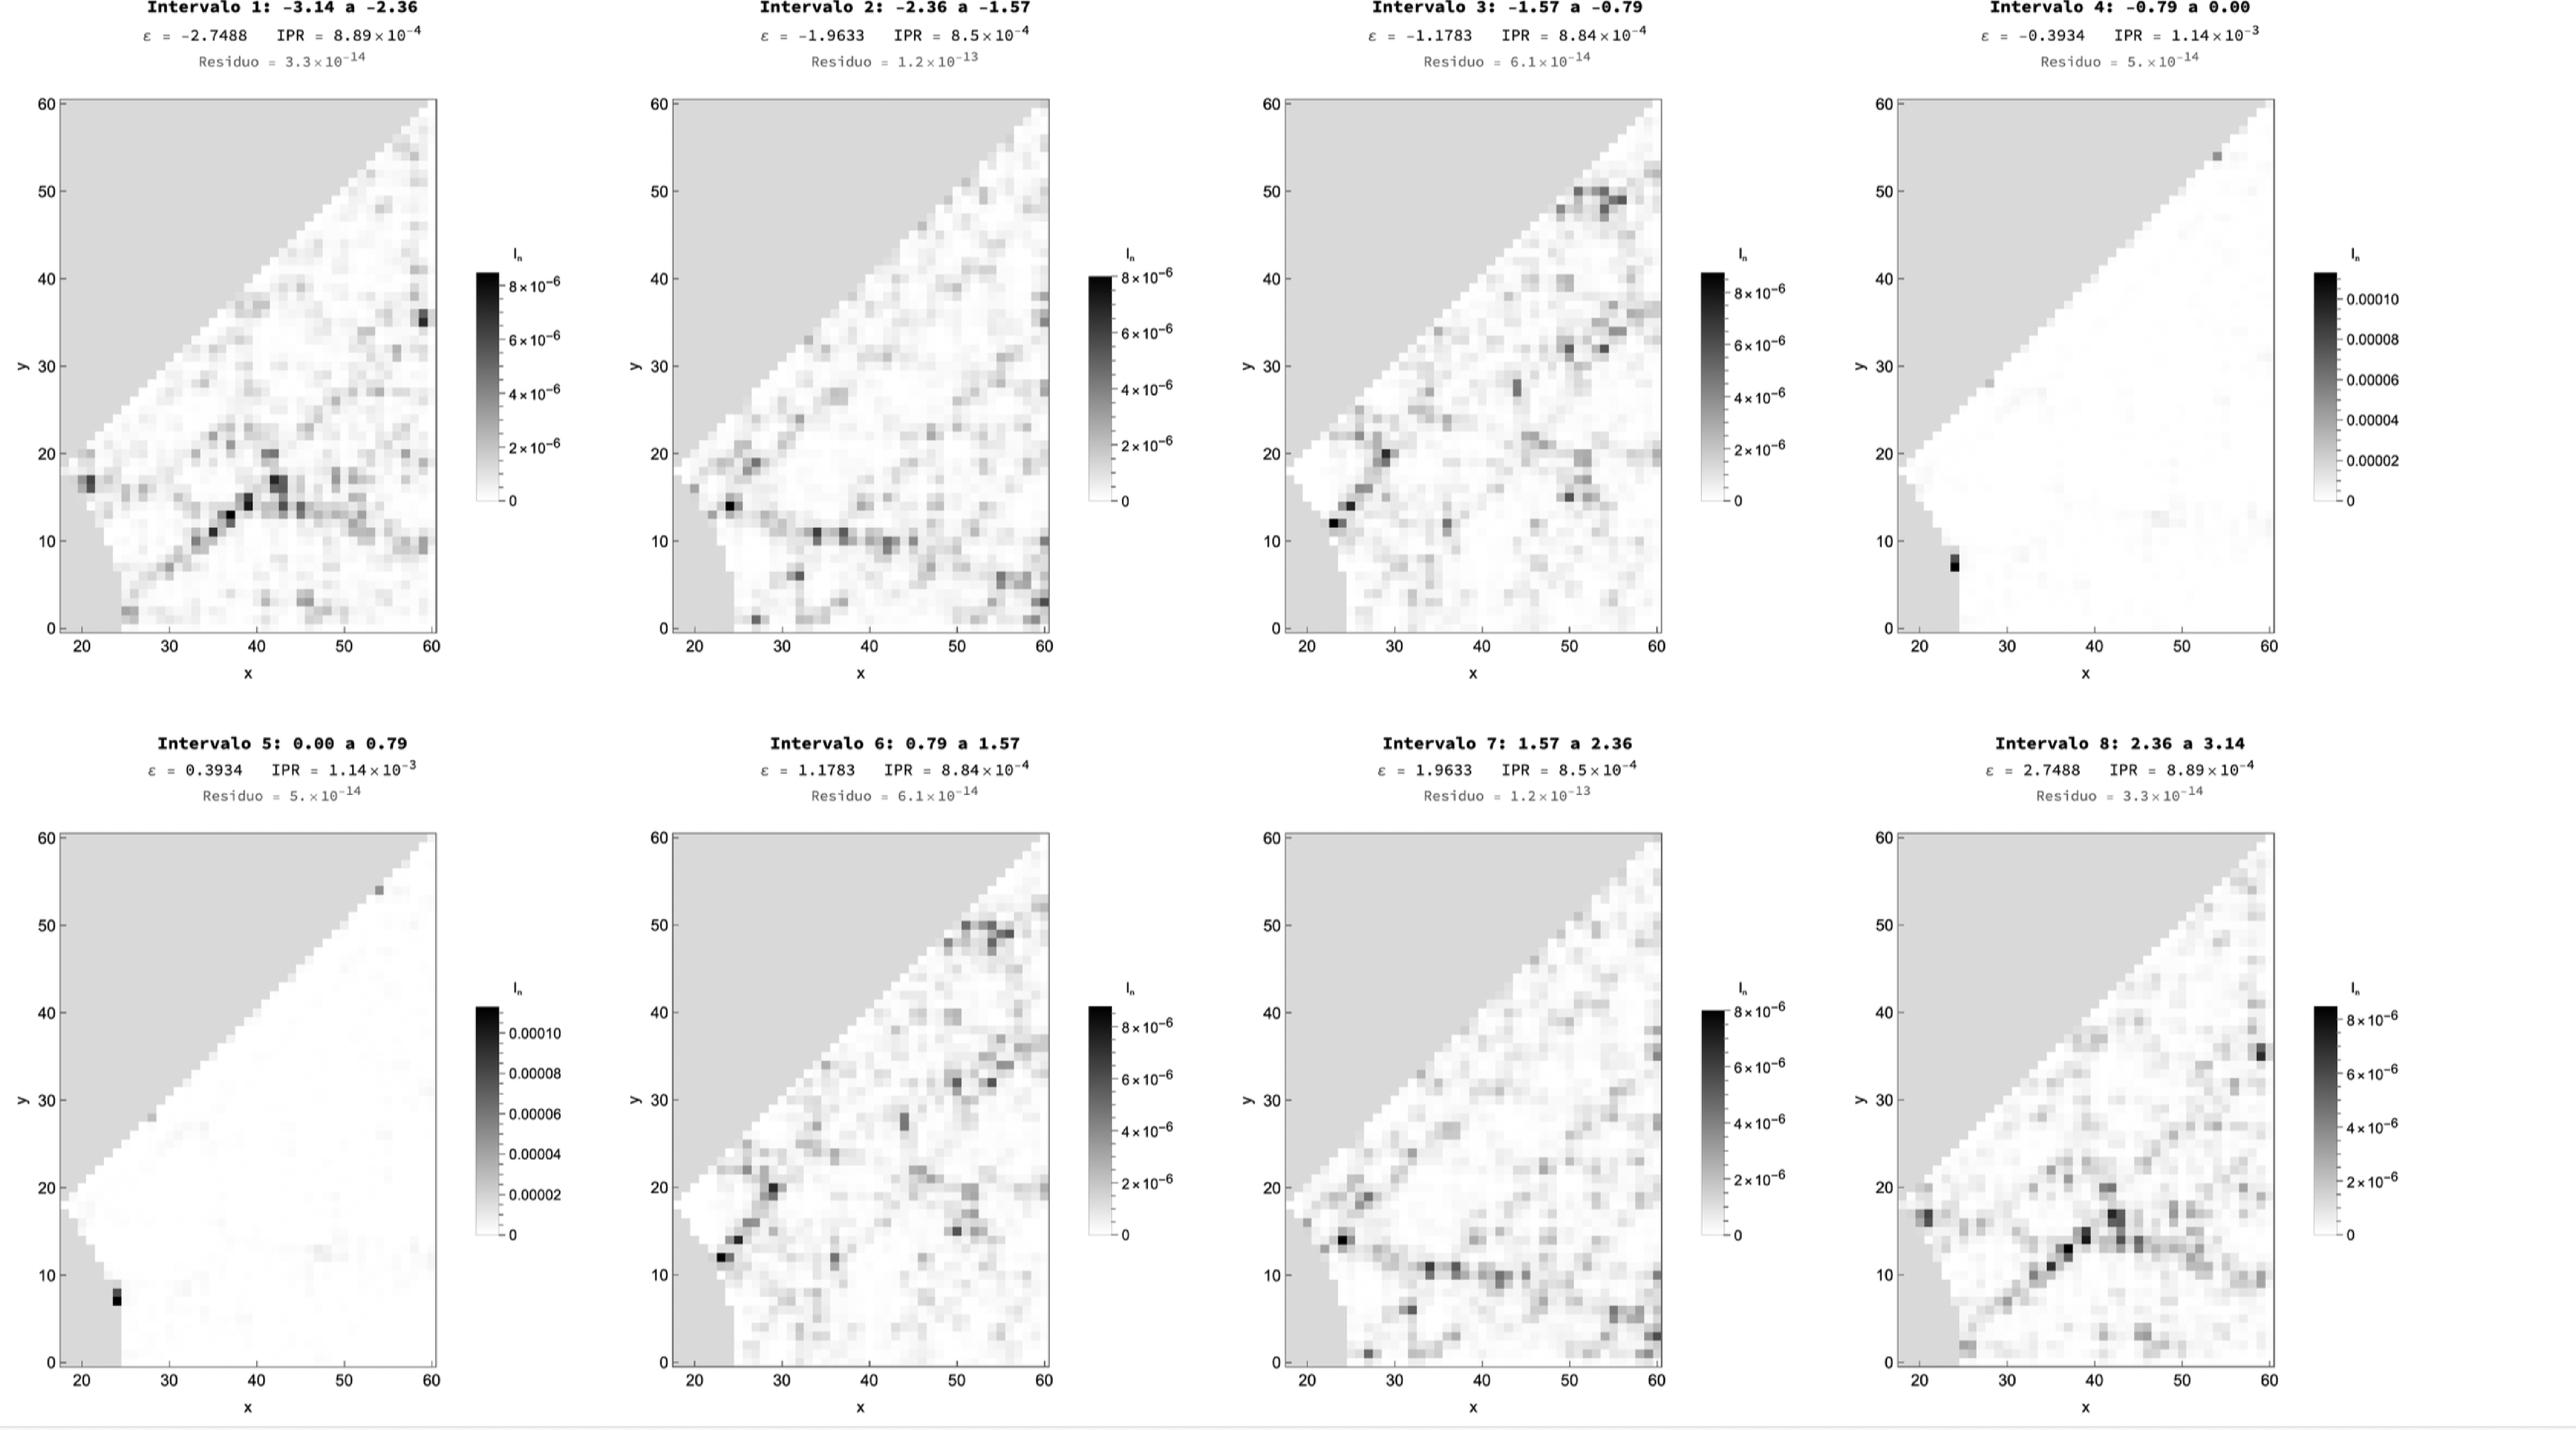
\includegraphics[trim={0.000bp 918.255bp 2480.438bp 0.000bp},clip,width=\linewidth,height=#1,keepaspectratio]{IPRDensity_Sinai_Intervals01-08.pdf}}
\expandafter\def\csname DensitySinaiFour\endcsname#1{%
  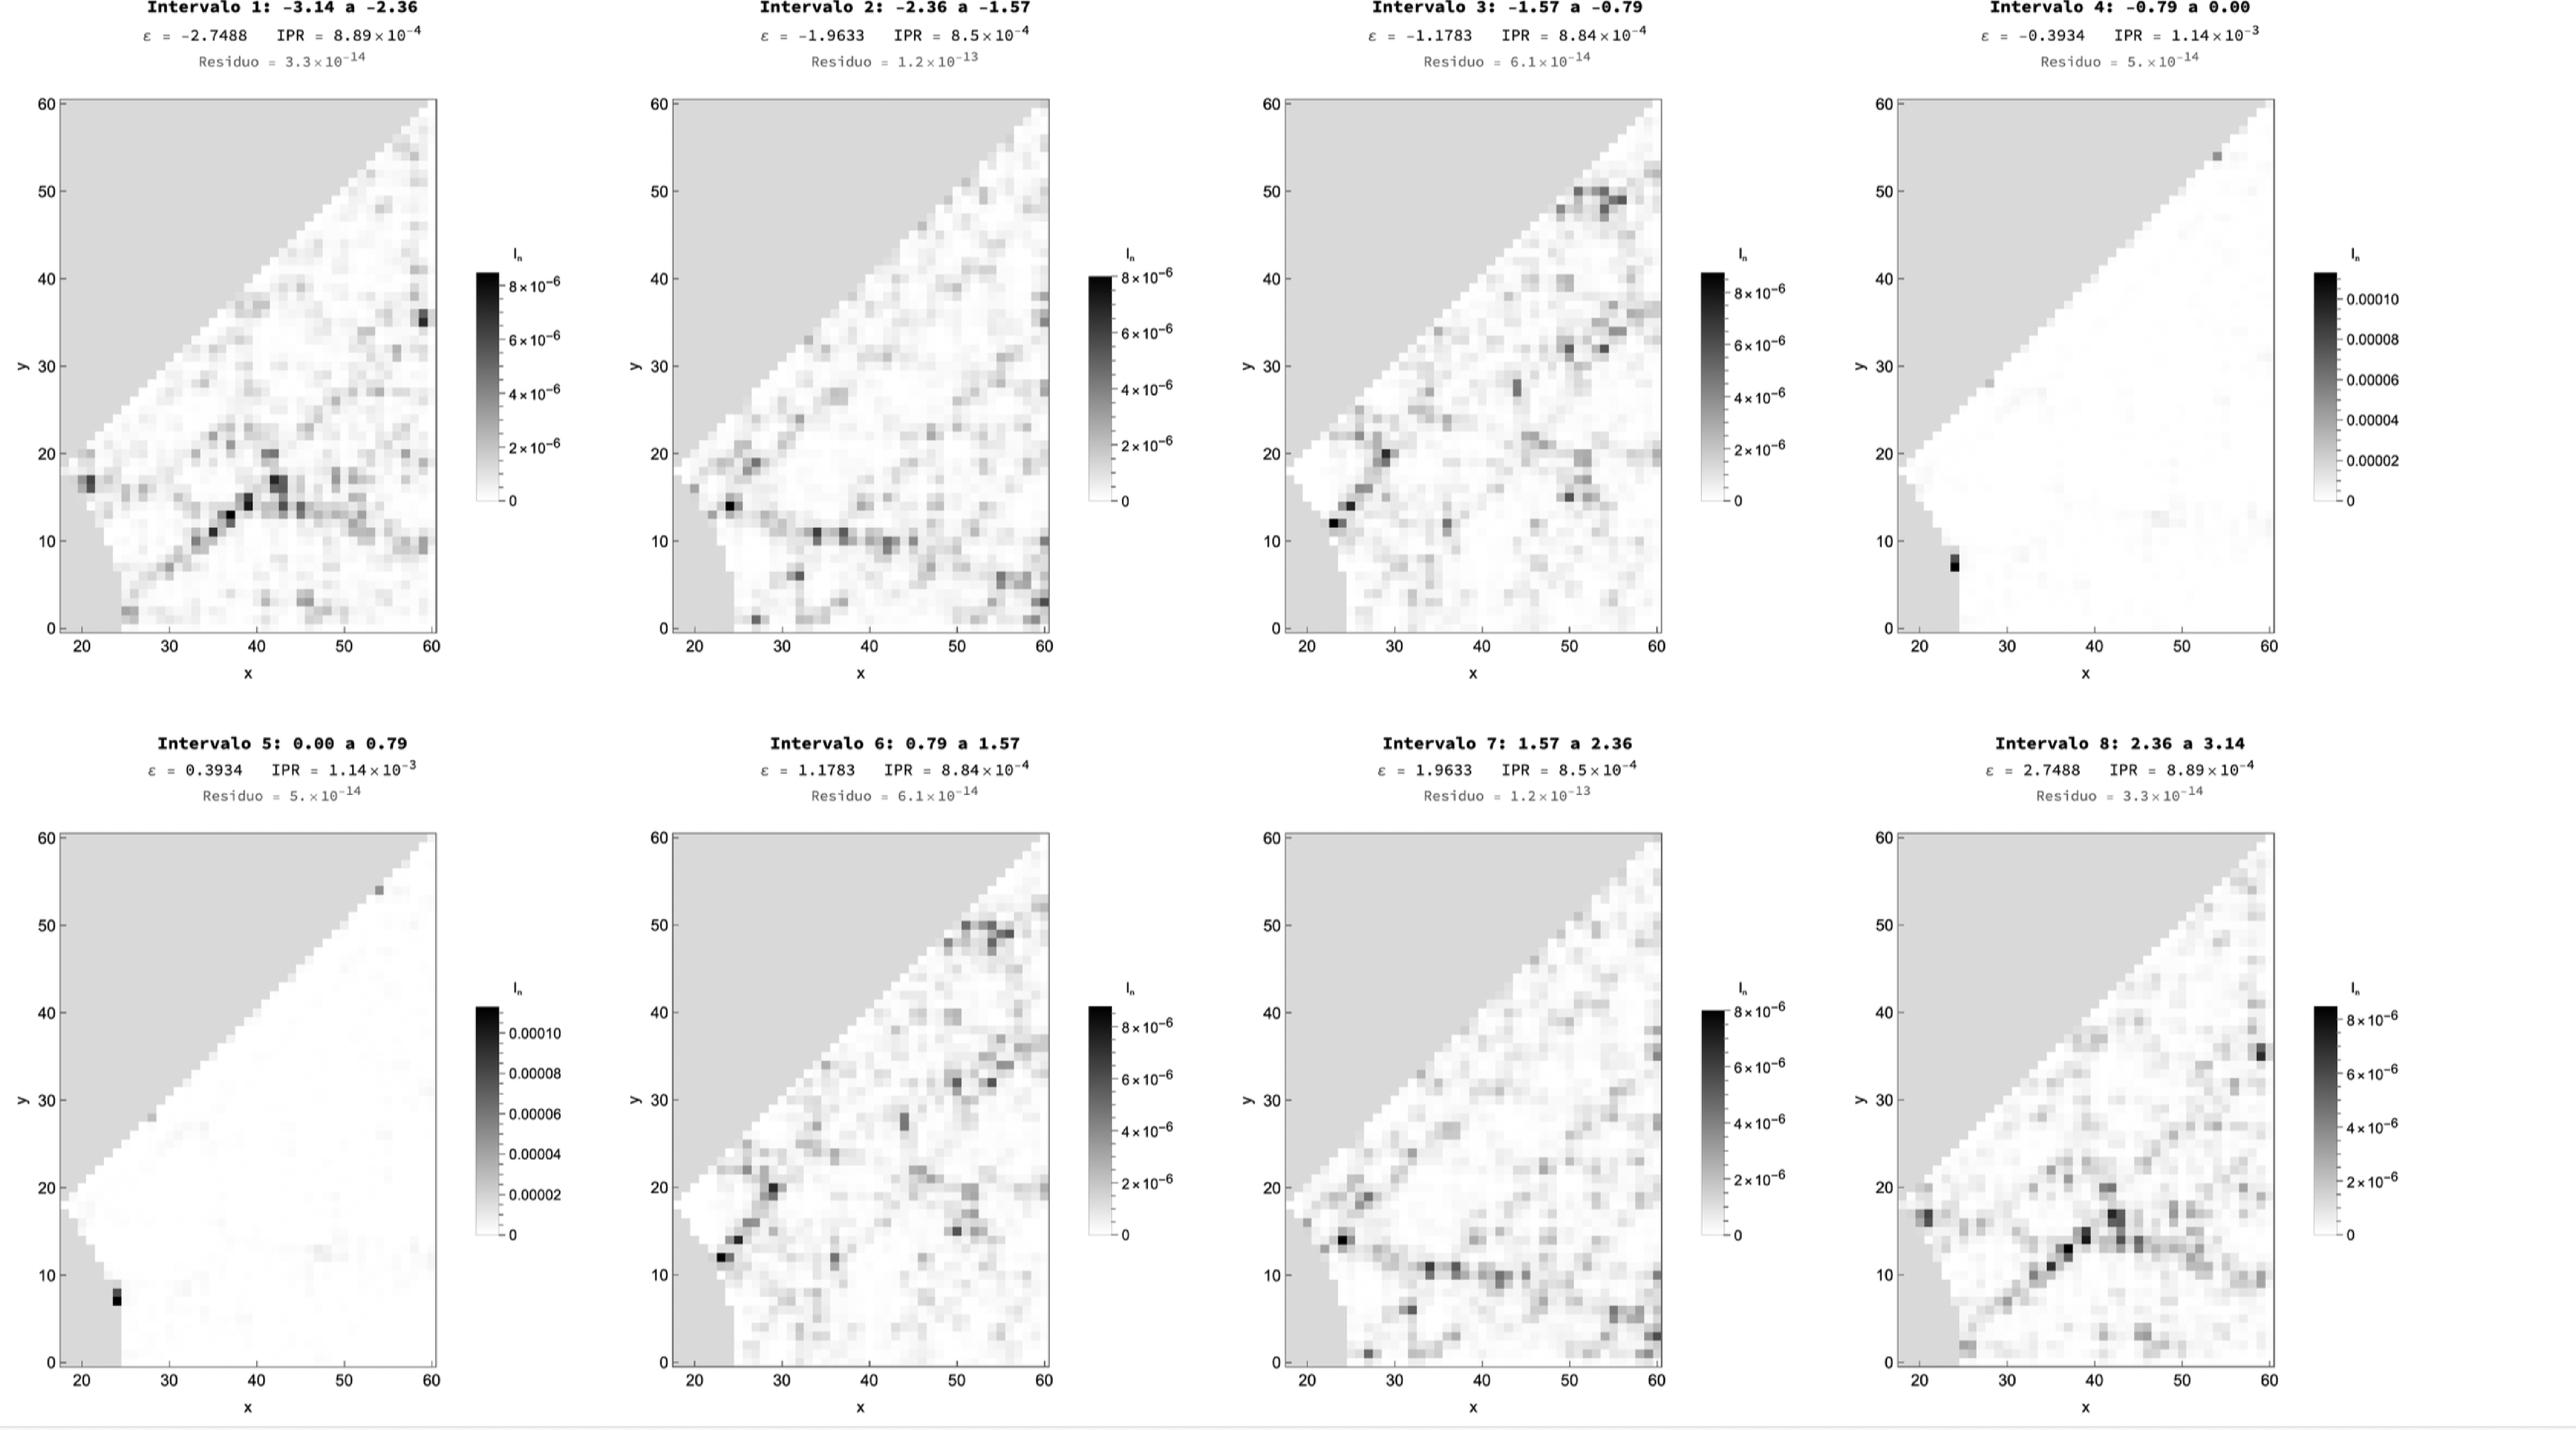
\includegraphics[trim={2480.438bp 918.255bp 0.000bp 0.000bp},clip,width=\linewidth,height=#1,keepaspectratio]{IPRDensity_Sinai_Intervals01-08.pdf}}

\newcommand{\TimeRow}[2]{%
  \noindent\begin{minipage}[c][#2][c]{.055\textwidth}\centering\small\coin{#1}\end{minipage}%
  \begin{minipage}[c][#2][c]{.445\textwidth}\centering\csname TimeRect#1\endcsname{#2}\end{minipage}\hfill
  \begin{minipage}[c][#2][c]{.445\textwidth}\centering\csname TimeSinai#1\endcsname{#2}\end{minipage}\par}
\newcommand{\TimePair}[2]{%
  \begin{frame}[t]{Promedio temporal: \coin{#1} y \coin{#2}}
    \GeoHeader\TimeRow{#1}{2.65cm}\TimeRow{#2}{2.65cm}
    \captionline{Cada mapa conserva su escala de probabilidad.}
  \end{frame}}

\hypersetup{pdftitle={Caminatas cuánticas en billares},
  pdfsubject={Resultados para discusión},
  pdfauthor={Investigación de caminatas cuánticas}}

\begin{document}

% ----------------------------------------------------------------------
% 1. Modelo y monedas
% ----------------------------------------------------------------------
\section{Modelo y monedas}
\begin{frame}[t]{Caminata cuántica en billares}
  \captionline{\Large El modelo a trabajar: }
  \vspace{2mm}
  \[
    \mathcal H=\mathcal H_p\otimes\mathcal H_c,
    \qquad \dim\mathcal H_p=N,\quad \dim\mathcal H_c=4
  \]
  \[
    \ket{\psi_t}=\sum_{v\in\Omega}\sum_{c=1}^{4}
      \psi_c(v,t)\ket{v}\otimes\ket{c}
  \]
  \[
    \boxed{\ket{\psi_{t+1}}=U\ket{\psi_t},\qquad
      U=S\bigl(\mathbb I_p\otimes C_4\bigr)}
  \]
  \begin{itemize}
    \item $C_4$ mezcla las cuatro direcciones de movimiento.
    \item $S$ desplaza al caminante e incorpora la reflexión en la frontera.
  \end{itemize}
\end{frame}

\begin{frame}[t]{Desplazamiento y geometrías}
  \noindent{\small Base de moneda: arriba, abajo, derecha e izquierda.}\par
  \[
    S\ket{v,c}=\begin{cases}
      \ket{v+\delta_c,c}, & v+\delta_c\in\Omega,\\
      \ket{v,\bar c}, & v+\delta_c\notin\Omega.
    \end{cases}
    \qquad \bar c:\ \uparrow\leftrightarrow\downarrow,\ \rightarrow\leftrightarrow\leftarrow
  \]
  \begin{columns}[T,onlytextwidth]
    \begin{column}{.485\textwidth}\centering
      \textbf{Rectángulo}\par\smallskip
      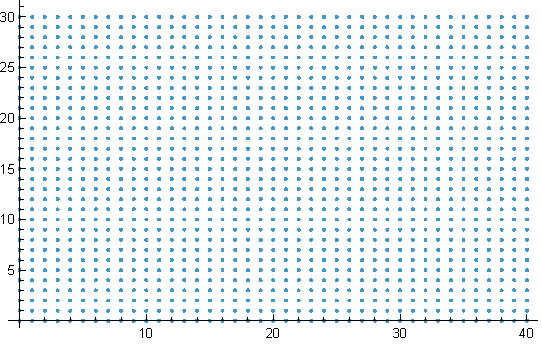
\includegraphics[width=.82\linewidth,height=2.55cm,keepaspectratio]{Stadium_Rect.pdf}
    \end{column}
    \begin{column}{.485\textwidth}\centering
      \textbf{Sinai}\par\smallskip
      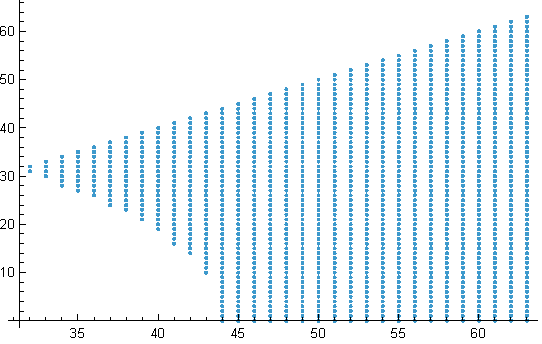
\includegraphics[width=.82\linewidth,height=2.55cm,keepaspectratio]{Stadium_Sinai.pdf}
    \end{column}
  \end{columns}
\end{frame}

\begin{frame}[t]{Las nueve monedas que se han trabajado}
  \noindent{\small La moneda permanece fija durante la evolución y es la misma en todos los sitios.}\par
  \vspace{1mm}
  \centering
  {\small\renewcommand{\arraystretch}{1.11}
  \begin{tabular}{@{}p{1.0cm}p{3.0cm}l@{}}
    \toprule
    Código & $C_4$ & Construcción\\\midrule
    \coin{gpg} & $GPG^\dagger$ & Fases diagonales mezcladas con Grover\\
    \coin{oo} & $O_1\otimes O_2$ & Producto de dos matrices COE de dimensión 2\\
    \coin{uoou} & $U(O_1\otimes O_2)U^\dagger$ & Conjugación unitaria de \coin{oo}\\
    \coin{o} & $O_4$ & Matriz del ensamble COE de dimensión 4\\
    \coin{b} & $B$ & Matriz fija y dispersa\\
    \coin{ubu} & $UBU^\dagger$ & Conjugación unitaria de \coin{b}\\
    \coin{u} & $U$ & Matriz del ensamble CUE de dimensión 4\\
    \coin{upu} & $UPU^\dagger$ & Conjugación unitaria de las fases diagonales\\
    \coin{p} & $P$ & Matriz diagonal de fases aleatorias\\\bottomrule
  \end{tabular}}
  \captionline{$P=\operatorname{diag}(e^{i\theta_1},\ldots,e^{i\theta_4})$, $\theta_j\sim\mathcal U[0,2\pi)$.
  $G$ es Grover a $\pi/4$ y $U$ es una matriz CUE.\\
  COE: ensamble circular ortogonal. CUE: ensamble circular unitario.}
  \takeaway{Cambiar la base de la moneda puede cambiar la caminata: el desplazamiento $S$ permanece fijo.}
\end{frame}

% ----------------------------------------------------------------------
% 2. Estadística espectral
% ----------------------------------------------------------------------
\section{Estadística espectral}

\SpectralPair{Espaciamientos: \coin{gpg} y \coin{oo}}{Ps}{gpg}{oo}
  {Rectángulo: tendencia a Poisson. Sinai: repulsión de niveles.}
\SpectralPair{Espaciamientos: \coin{uoou} y \coin{o}}{Ps}{uoou}{o}
  {Comparación de los datos con Poisson, GOE/COE y GUE/CUE.}
\SpectralPair{Espaciamientos: \coin{b} y \coin{ubu}}{Ps}{b}{ubu}
  {La conjugación de $B$ cambia su orientación respecto a las direcciones del desplazamiento.}
\SpectralPair{Espaciamientos: \coin{u} y \coin{upu}}{Ps}{u}{upu}
  {Comparación entre una moneda CUE y una moneda diagonal conjugada por una matriz CUE.}

\begin{frame}[t]{Espaciamientos: \coin{p}}
  \GeoHeader\SpectralRow{Ps}{p}\SpectralModifiedRow
  \captionline{\coin{pModif}: primer bin excluido (96.74\% en rectángulo; 49.61\% en Sinai).}
\end{frame}

% P(r) y SFF siguen las mismas parejas y columnas que P(s).
\SpectralPair{Razones de espaciamientos: \coin{gpg} y \coin{oo}}{Pr}{gpg}{oo}
  {$r\in[0,1]$. Las razones usan los espaciamientos originales, sin unfolding.}
\SpectralPair{Razones de espaciamientos: \coin{uoou} y \coin{o}}{Pr}{uoou}{o}
  {Comparación con las referencias indicadas en las leyendas.}
\SpectralPair{Razones de espaciamientos: \coin{b} y \coin{ubu}}{Pr}{b}{ubu}
  {Comparación con las referencias indicadas en las leyendas.}
\SpectralPair{Razones de espaciamientos: \coin{u} y \coin{upu}}{Pr}{u}{upu}
  {Comparación con las referencias indicadas en las leyendas.}
\SpectralSingle{Razones de espaciamientos: \coin{p}}{Pr}{p}
  {$r\in[0,1]$. Las razones usan los espaciamientos originales, sin unfolding.}

\SpectralPair{SFF: \coin{gpg} y \coin{oo}}{SFF}{gpg}{oo}
  {Gris: promedio entre realizaciones. Azul: promedio con ventana temporal. Punteado: COE.}
\SpectralPair{SFF: \coin{uoou} y \coin{o}}{SFF}{uoou}{o}
  {Las escalas verticales pueden cambiar entre paneles.}
\SpectralPair{SFF: \coin{b} y \coin{ubu}}{SFF}{b}{ubu}
  {Las escalas verticales pueden cambiar entre paneles.}
\SpectralPair{SFF: \coin{u} y \coin{upu}}{SFF}{u}{upu}
  {La referencia COE se conserva tal como aparece en las figuras originales.}
\SpectralSingle{SFF: \coin{p}}{SFF}{p}
  {Las escalas verticales pueden cambiar entre paneles.}

\begin{frame}[t]{Resumen de la estadística espectral según la geometría}
  \small
  \setlength{\tabcolsep}{3pt}
  \renewcommand{\arraystretch}{1.3}
  \begin{tabular}{@{}p{2.0cm}p{6.0cm}p{5.8cm}@{}}
    \textbf{Monedas} & \textbf{Rectángulo} & \textbf{Sinai}\\
    \midrule
    \coin{gpg}, \coin{oo} & Comportamiento próximo a Poisson\newline visto en P(s), P(r) y SFF.
      & La estadística sugiere que sigue COE.\\
    \coin{b} & Los resultados sugieren que su espectro sigue \newline una estadística de Poisson.
      & La estadística sugiere que sigue CUE\\
    \coin{uoou}, \coin{o}, \coin{ubu}, \coin{u}, \coin{upu}
      & La estadística sigue las predicciones de COE &  La estadística sigue las predicciones del CUE.\\
    \coin{p} & Presenta degeneneraciones masivas\newline
      Es dificil hacer la estadística correspondiente para la P(s) y P(r)
      & Habiendo removido artificialmente espaciamientos nulos\newline
      se ve una aparente repulsión de niveles.\\
  \end{tabular}
\end{frame}

% ----------------------------------------------------------------------
% 3. Localización espacial y entrelazamiento
% ----------------------------------------------------------------------
\section{IPR espacial}
\begin{frame}[t]{IPR espacial: estado inicial localizado}
  \[
    P_t(v)=\sum_{c=1}^{4}|\psi_c(v,t)|^2,
    \qquad \mathrm{IPR}_{\mathrm{esp}}(t)=\sum_{v\in\Omega}P_t(v)^2.
  \]
  \vspace{-1mm}
  \ComparePlots{IPR_Comparacion_Rect.pdf}{IPR_Comparacion_Sinai.pdf}
    {$97\times60$, $2000$ pasos.}{$L=140$, $R=100$, $2000$ pasos.}
  \captionline{IPR alto: mayor concentración espacial. Una distribución uniforme tiene IPR $=1/N$.}
\end{frame}

\begin{frame}[t]{IPR espacial: estado inicial deslocalizado}
  \ComparePlots{IPR_Comparacion_Rect_Deslocalizado.pdf}{IPR_Comparacion_Sinai_Deslocalizado.pdf}
    {$97\times60$, $2000$ pasos.}{$L=140$, $R=100$, $2000$ pasos.}
  \takeaway{Con este estado inicial, las curvas de las monedas quedan mucho más próximas.}
  \captionline{Las líneas de referencia pertenecen a las figuras originales. El IPR suma primero las probabilidades de moneda en cada sitio.}
\end{frame}

\section{Entrelazamiento}
\begin{frame}[t]{Entrelazamiento: estado inicial localizado}
  \[
    \rho_c(t)=\operatorname{Tr}_p\ket{\psi_t}\bra{\psi_t},
    \qquad S_c(t)=-\operatorname{Tr}[\rho_c(t)\ln\rho_c(t)].
  \]
  \ComparePlots{EntanglementEntropy_Rect.pdf}{EntanglementEntropy_Sinai.pdf}
    {$80\times50$, $1000$ pasos.}{$L=120$, $R=90$, $1000$ pasos.}
  \captionline{La entropía usa logaritmos naturales. El máximo para la moneda de dimensión 4 es $\ln4\simeq1.386$.}
\end{frame}

\begin{frame}[t]{Entrelazamiento: estado inicial deslocalizado}
  \ComparePlots{EntanglementEntropy_Rect_Deslocalizado.pdf}{EntanglementEntropy_Sinai_Deslocalizado.pdf}
    {$80\times50$, $1000$ pasos.}{$L=120$, $R=90$, $1000$ pasos.}
  \takeaway{Varias monedas con estadística espectral distinta alcanzan entropías cercanas a $\ln4$.}
  \captionline{El entrelazamiento por sí solo no determina la clasificación espectral.}
\end{frame}

% ----------------------------------------------------------------------
% 4. Promedio temporal y eigenestados
% ----------------------------------------------------------------------
\section{Promedio temporal}
\begin{frame}[t]{Promedio y límite temporal}
  \noindent{\small
  $\displaystyle\overline P_T(v)=\frac1T\sum_{t=0}^{T-1}P_t(v),
  \qquad \pi(v)=\lim_{T\to\infty}\overline P_T(v).$}\par
  \GeoHeader\TimeRow{gpg}{4.45cm}
  \captionline{Rectángulo: $100\times87$. Sinai: $L=120$, $R=90$. Cada mapa tiene su propia escala.}
  \takeaway{Los mapas muestran promedios finitos. La comprobación de convergencia al límite queda abierta.}
\end{frame}

\section{Eigenestados}
\begin{frame}[t]{Densidad espacial del IPR de los eigenestados}
  \noindent{\small
  $\displaystyle p_n(v)=\sum_c|\langle v,c|\phi_n\rangle|^2,
  \qquad I_n(v)=p_n(v)^2,\qquad\mathrm{IPR}_n=\sum_v I_n(v).$}\par
  \begin{columns}[T,onlytextwidth]
    \begin{column}{.485\textwidth}\centering
      {\small\bfseries Rectángulo}\par\smallskip
      \csname DensityRectSeven\endcsname{4.25cm}
    \end{column}
    \begin{column}{.485\textwidth}\centering
      {\small\bfseries Sinai}\par\smallskip
      \csname DensitySinaiFour\endcsname{4.25cm}
    \end{column}
  \end{columns}
  \captionline{Ejemplos de concentración cerca de la frontera. Oscuro significa mayor contribución local al IPR. Las escalas y los tamaños son distintos.}
\end{frame}

\section{Discusión}
\begin{frame}[t]{Resultados para discutir}
  \begin{itemize}
    \setlength\itemsep{4mm}
    \item La comparación entre geometrías requiere considerar también la moneda.
    \item El estado inicial afecta la separación entre las curvas de IPR y entrelazamiento.
    \item Los eigenestados permiten examinar dónde se concentra la probabilidad.
  \end{itemize}
  \vspace{3mm}

\end{frame}

% ----------------------------------------------------------------------
% Apéndice: consultas durante la reunión, fuera del recorrido principal.
% ----------------------------------------------------------------------
\ifapendice
\appendix
\section{Apéndice espectral}
\begin{frame}[t]{Apéndice: detalle de las comparaciones}
  \textbf{Orden de monedas}\par
  \coin{gpg}, \coin{oo}, \coin{uoou}, \coin{o}, \coin{b}, \coin{ubu}, \coin{u}, \coin{upu}, \coin{p}.
  \vspace{4mm}
  \begin{itemize}
    \item DoS y unfolding para las nueve monedas.
    \item $P(r)$ para las nueve monedas.
    \item SFF para las nueve monedas.
    \item Promedios temporales restantes y mapas completos de eigenestados.
  \end{itemize}
  \captionline{El apéndice permite consultar el detalle sin alargar el recorrido principal.}
\end{frame}

\SpectralPair{DoS y unfolding: \coin{gpg} y \coin{oo}}{DoS}{gpg}{oo}{Densidad de eigenfases y transformación de unfolding de las figuras originales.}
\SpectralPair{DoS y unfolding: \coin{uoou} y \coin{o}}{DoS}{uoou}{o}{Cada panel conserva sus ejes originales.}
\SpectralPair{DoS y unfolding: \coin{b} y \coin{ubu}}{DoS}{b}{ubu}{Cada panel conserva sus ejes originales.}
\SpectralPair{DoS y unfolding: \coin{u} y \coin{upu}}{DoS}{u}{upu}{Cada panel conserva sus ejes originales.}
\SpectralSingle{DoS y unfolding: \coin{p}}{DoS}{p}{Cada panel conserva sus ejes originales.}

\SpectralPair{Razones de espaciamientos: \coin{gpg} y \coin{oo}}{Pr}{gpg}{oo}{$r\in[0,1]$. Las razones usan los espaciamientos originales, sin unfolding.}
\SpectralPair{Razones de espaciamientos: \coin{uoou} y \coin{o}}{Pr}{uoou}{o}{Comparación con las referencias indicadas en las leyendas.}
\SpectralPair{Razones de espaciamientos: \coin{b} y \coin{ubu}}{Pr}{b}{ubu}{Comparación con las referencias indicadas en las leyendas.}
\SpectralPair{Razones de espaciamientos: \coin{u} y \coin{upu}}{Pr}{u}{upu}{Comparación con las referencias indicadas en las leyendas.}
\SpectralSingle{Razones de espaciamientos: \coin{p}}{Pr}{p}{$r\in[0,1]$. Las razones usan los espaciamientos originales, sin unfolding.}

\begin{frame}[t]{Factor de forma espectral}
  \[
    K(t)=\frac1{D}\left|\sum_{n=1}^{D}e^{-it\varepsilon_n}\right|^2,
    \qquad\tau=\frac{t}{D}.
  \]
  \noindent{\small $D$ es el número de niveles incluidos en el cálculo del SFF.}\par
  \begin{itemize}
    \item El SFF examina correlaciones espectrales a distintas escalas temporales.
    \item Las curvas guardadas incluyen promedio entre realizaciones y suavizado temporal.
    \item La leyenda original muestra la referencia COE utilizada en estos cálculos.
  \end{itemize}
  \captionline{El eje de las figuras usa $N$ para el número de niveles. Aquí se llama $D$ para distinguirlo del número de sitios.}
\end{frame}
\SpectralPair{SFF: \coin{gpg} y \coin{oo}}{SFF}{gpg}{oo}{Gris: promedio entre realizaciones. Azul: promedio con ventana temporal. Punteado: COE.}
\SpectralPair{SFF: \coin{uoou} y \coin{o}}{SFF}{uoou}{o}{Las escalas verticales pueden cambiar entre paneles.}
\SpectralPair{SFF: \coin{b} y \coin{ubu}}{SFF}{b}{ubu}{Las escalas verticales pueden cambiar entre paneles.}
\SpectralPair{SFF: \coin{u} y \coin{upu}}{SFF}{u}{upu}{La referencia COE se conserva tal como aparece en las figuras originales.}
\SpectralSingle{SFF: \coin{p}}{SFF}{p}{Las escalas verticales pueden cambiar entre paneles.}

\section{Apéndice temporal}
\begin{frame}[t]{Expresión del límite del promedio temporal}
  \noindent{\small Sea $\Pi_\lambda$ el proyector sobre el subespacio de eigenvalor $\lambda$ de $U$.}\par
  \[
    \lim_{T\to\infty}\frac1T\sum_{t=0}^{T-1}
      U^t\rho_0 U^{-t}
    =\sum_{\lambda}\Pi_\lambda\rho_0\Pi_\lambda,
    \qquad\rho_0=\ket{\psi_0}\bra{\psi_0}.
  \]
  \[
    \pi(v)=\sum_{c,\lambda}
      \left|\bra{v,c}\Pi_\lambda\ket{\psi_0}\right|^2.
  \]
  \captionline{El promedio elimina interferencias entre eigenvalores distintos. Conserva las coherencias dentro de los subespacios degenerados.}
  \captionline{Referencia de las notas originales: Aharonov et al., \emph{Quantum Walks on Graphs} (2001), arXiv:quant-ph/0012090.}
\end{frame}
\begin{frame}[t]{Promedio temporal: \coin{oo}}
  \GeoHeader\TimeRow{oo}{5.25cm}
  \captionline{Cada mapa conserva su escala de probabilidad.}
\end{frame}
\TimePair{uoou}{o}
\TimePair{b}{ubu}
\TimePair{u}{upu}
\begin{frame}[t]{Promedio temporal: \coin{p}}
  \GeoHeader\TimeRow{p}{5.25cm}
  \captionline{Cada mapa conserva su escala de probabilidad.}
\end{frame}

\section{Apéndice de eigenestados}
\begin{frame}[t]{Eigenestados: rectángulo, intervalos 4 a 9}
  \centering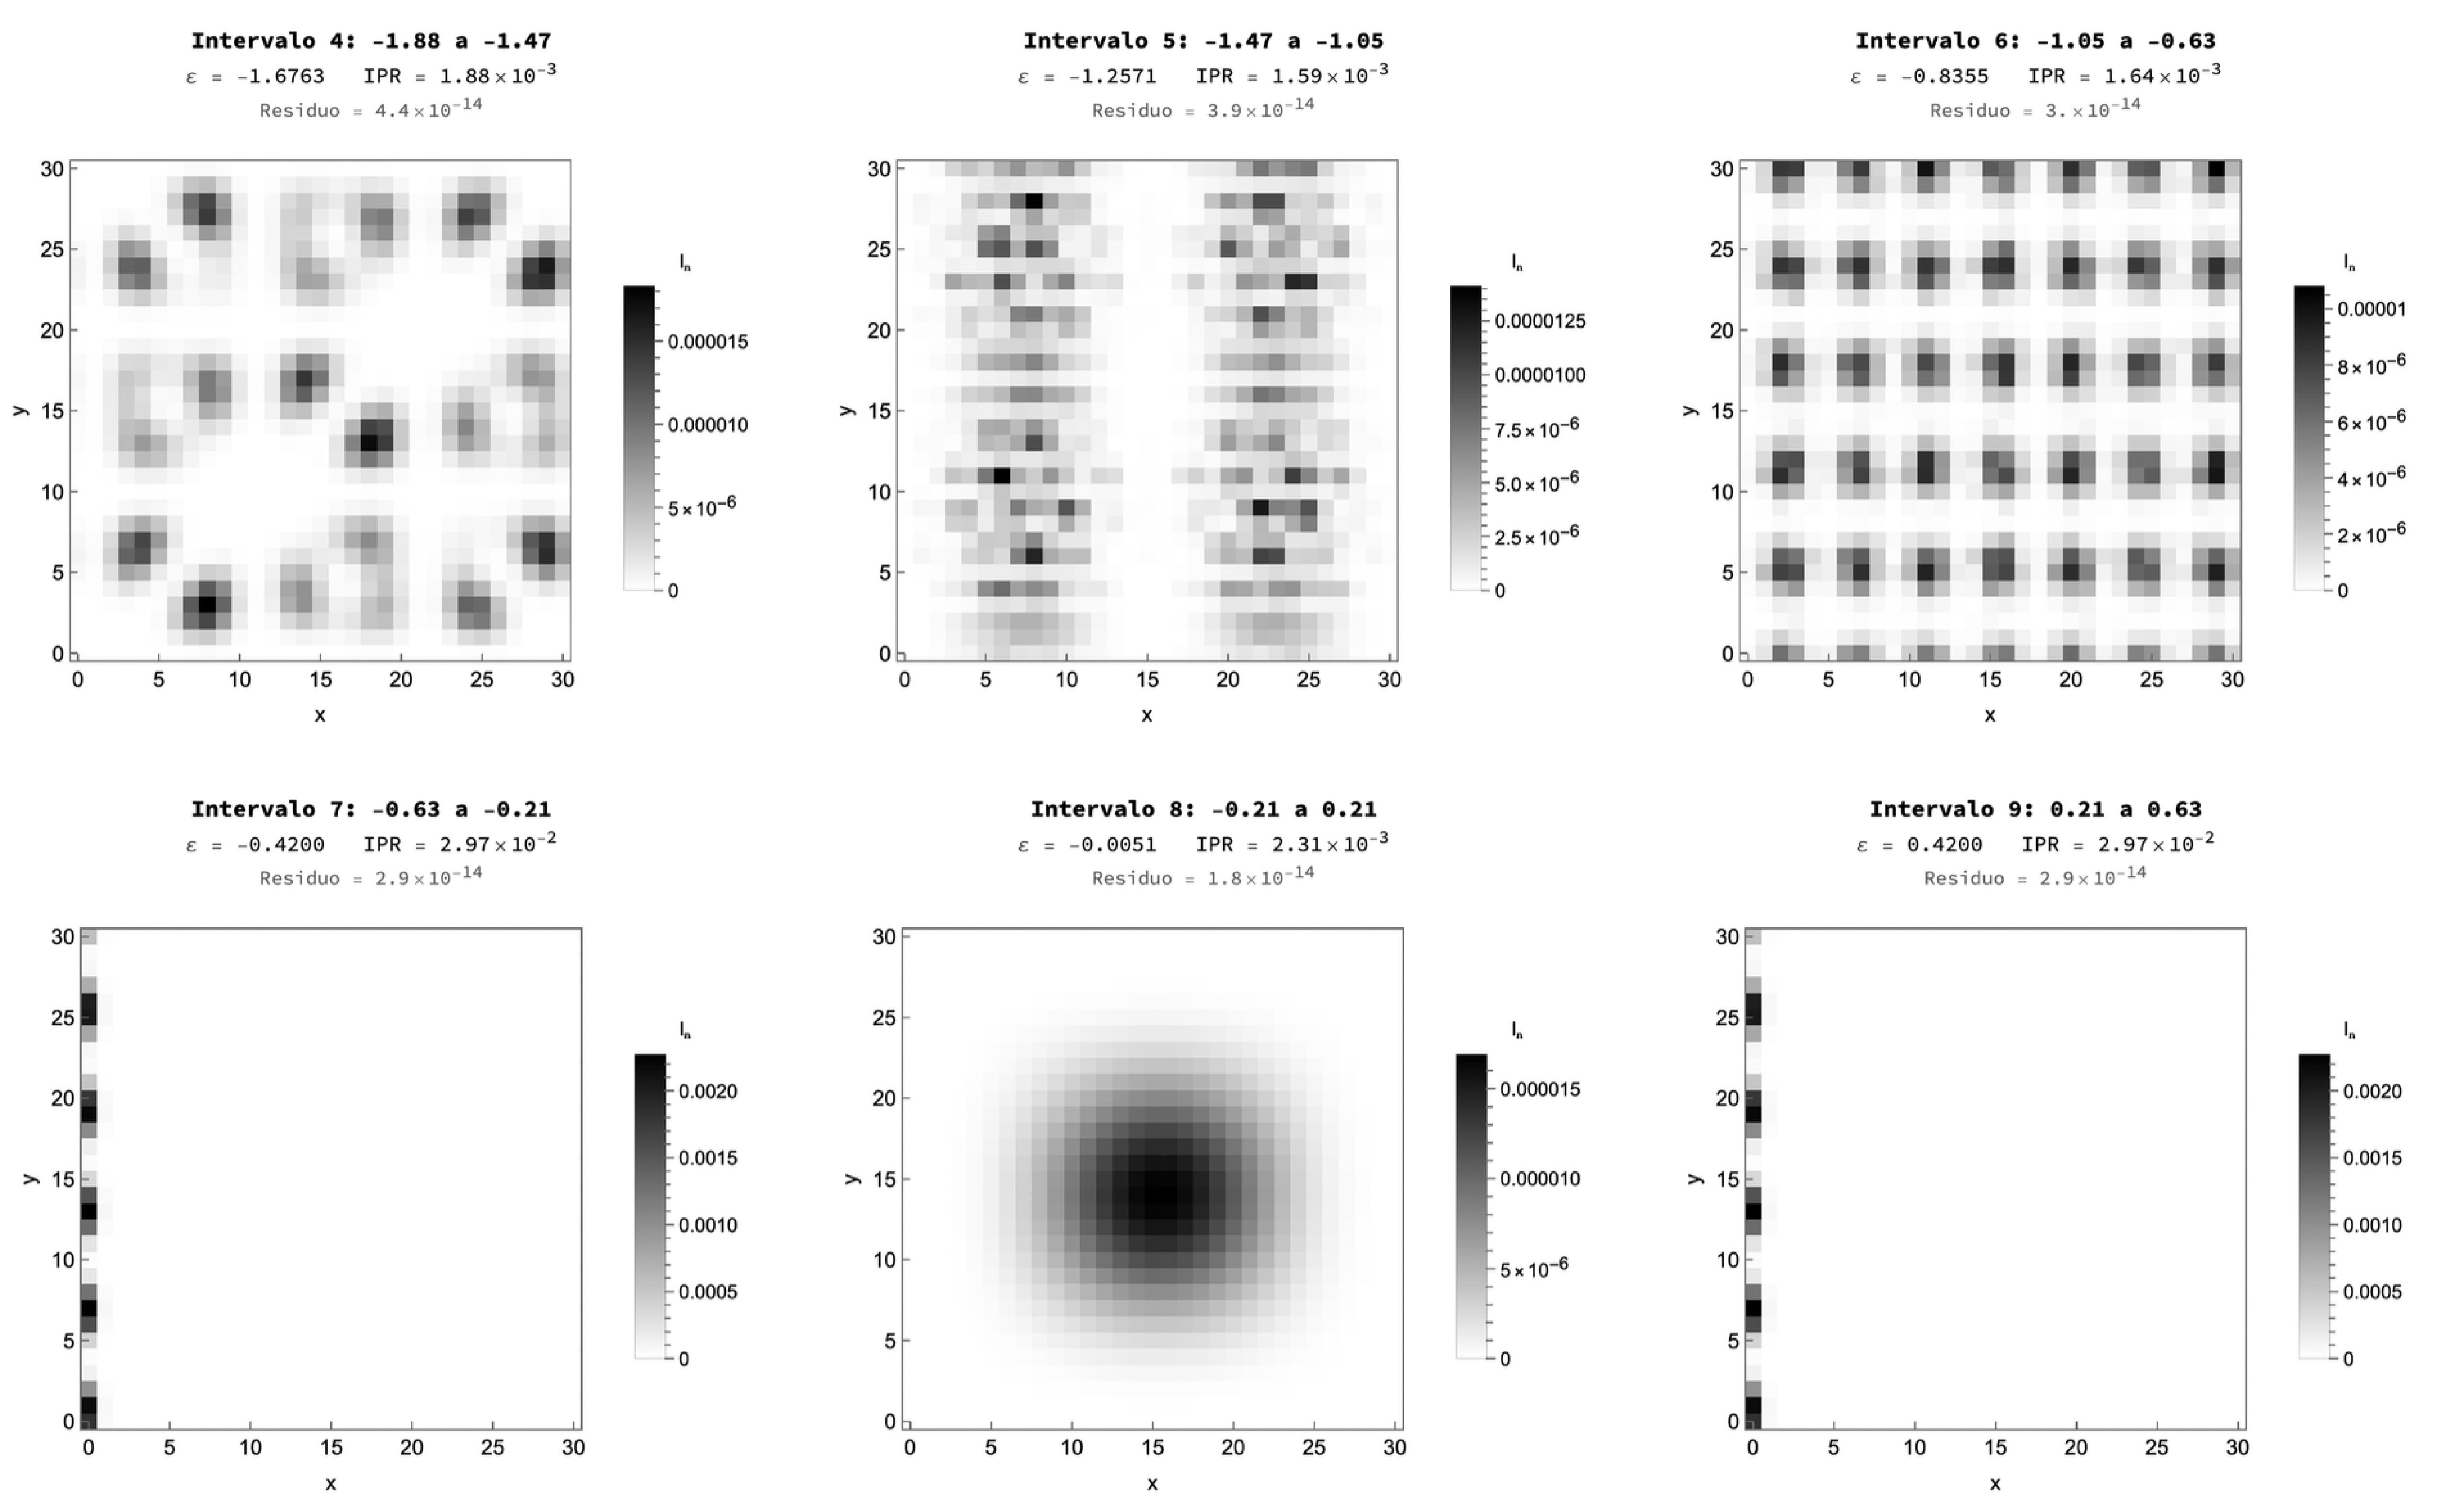
\includegraphics[width=\textwidth,height=5.7cm,keepaspectratio]{IPRDensity_Rect_Intervals04-09.pdf}
  \captionline{Cada panel indica eigenfase, IPR y residuo numérico. Cada mapa tiene su propia escala.}
\end{frame}
\begin{frame}[t]{Eigenestados: rectángulo, intervalos 10 a 15}
  \centering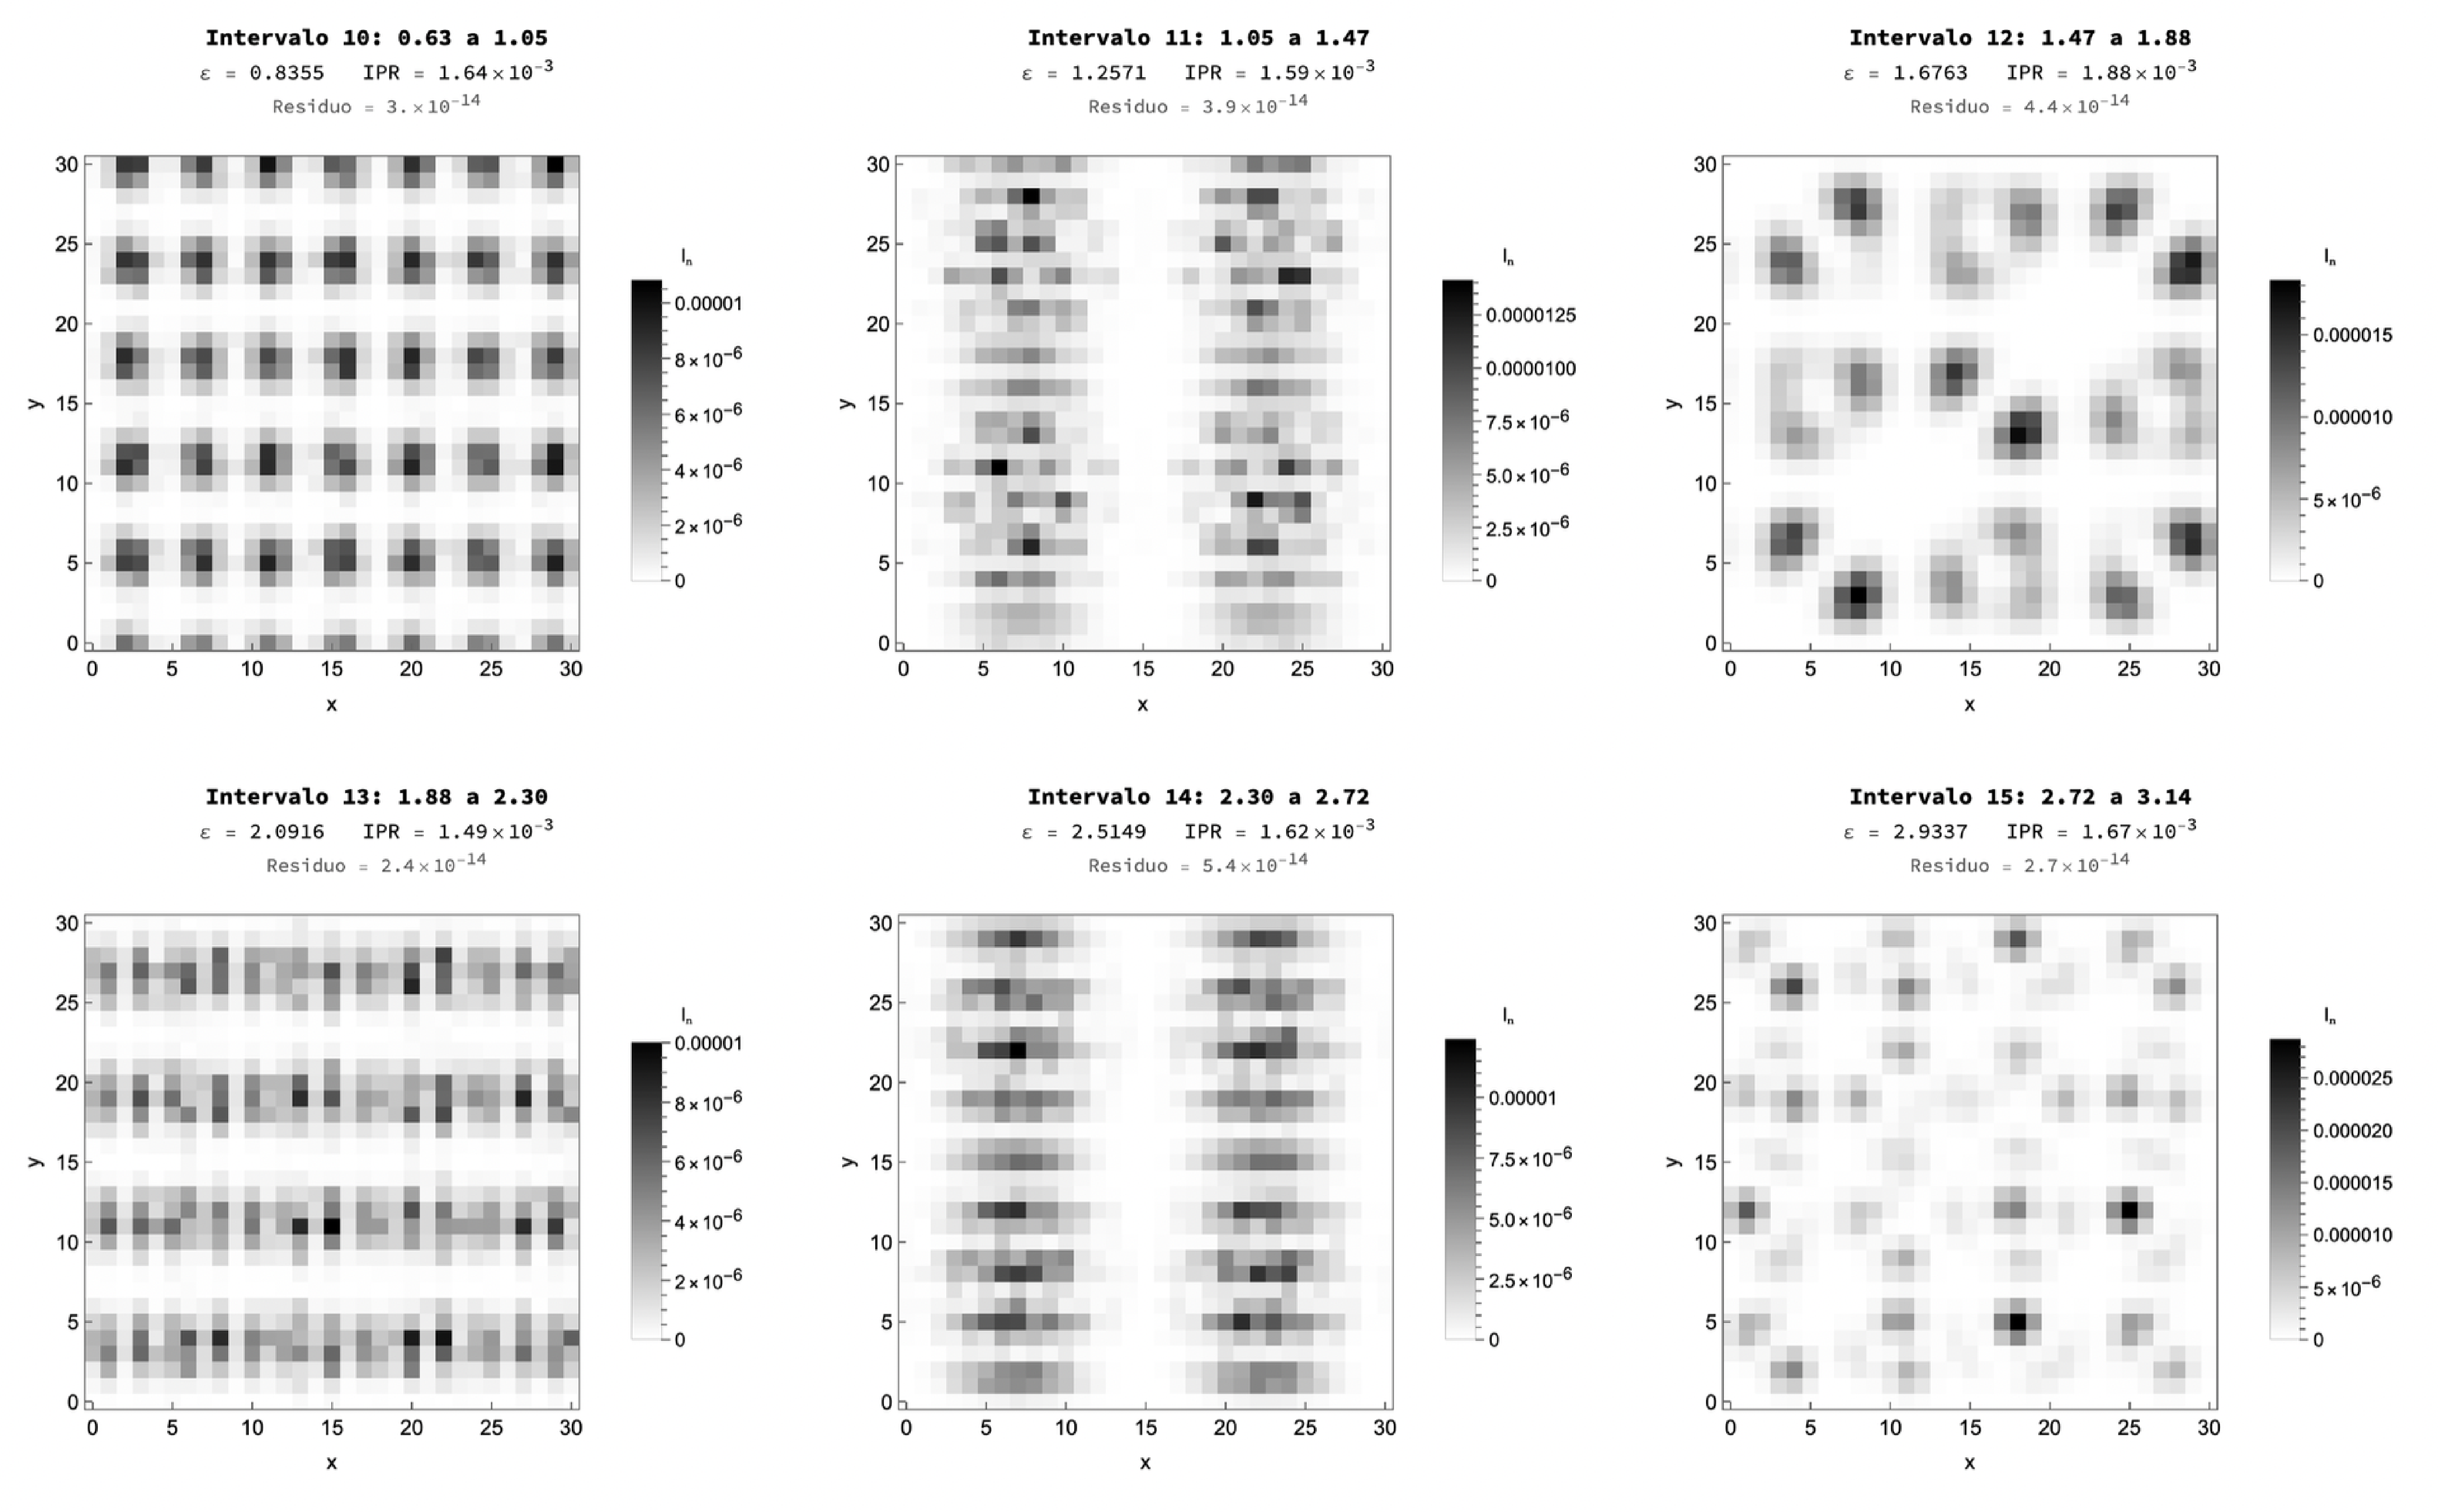
\includegraphics[width=\textwidth,height=5.7cm,keepaspectratio]{IPRDensity_Rect_Intervals10-15.pdf}
  \captionline{Cada panel indica eigenfase, IPR y residuo numérico. Cada mapa tiene su propia escala.}
\end{frame}
\begin{frame}[t]{Eigenestados: Sinai, intervalos 1 a 8}
  \centering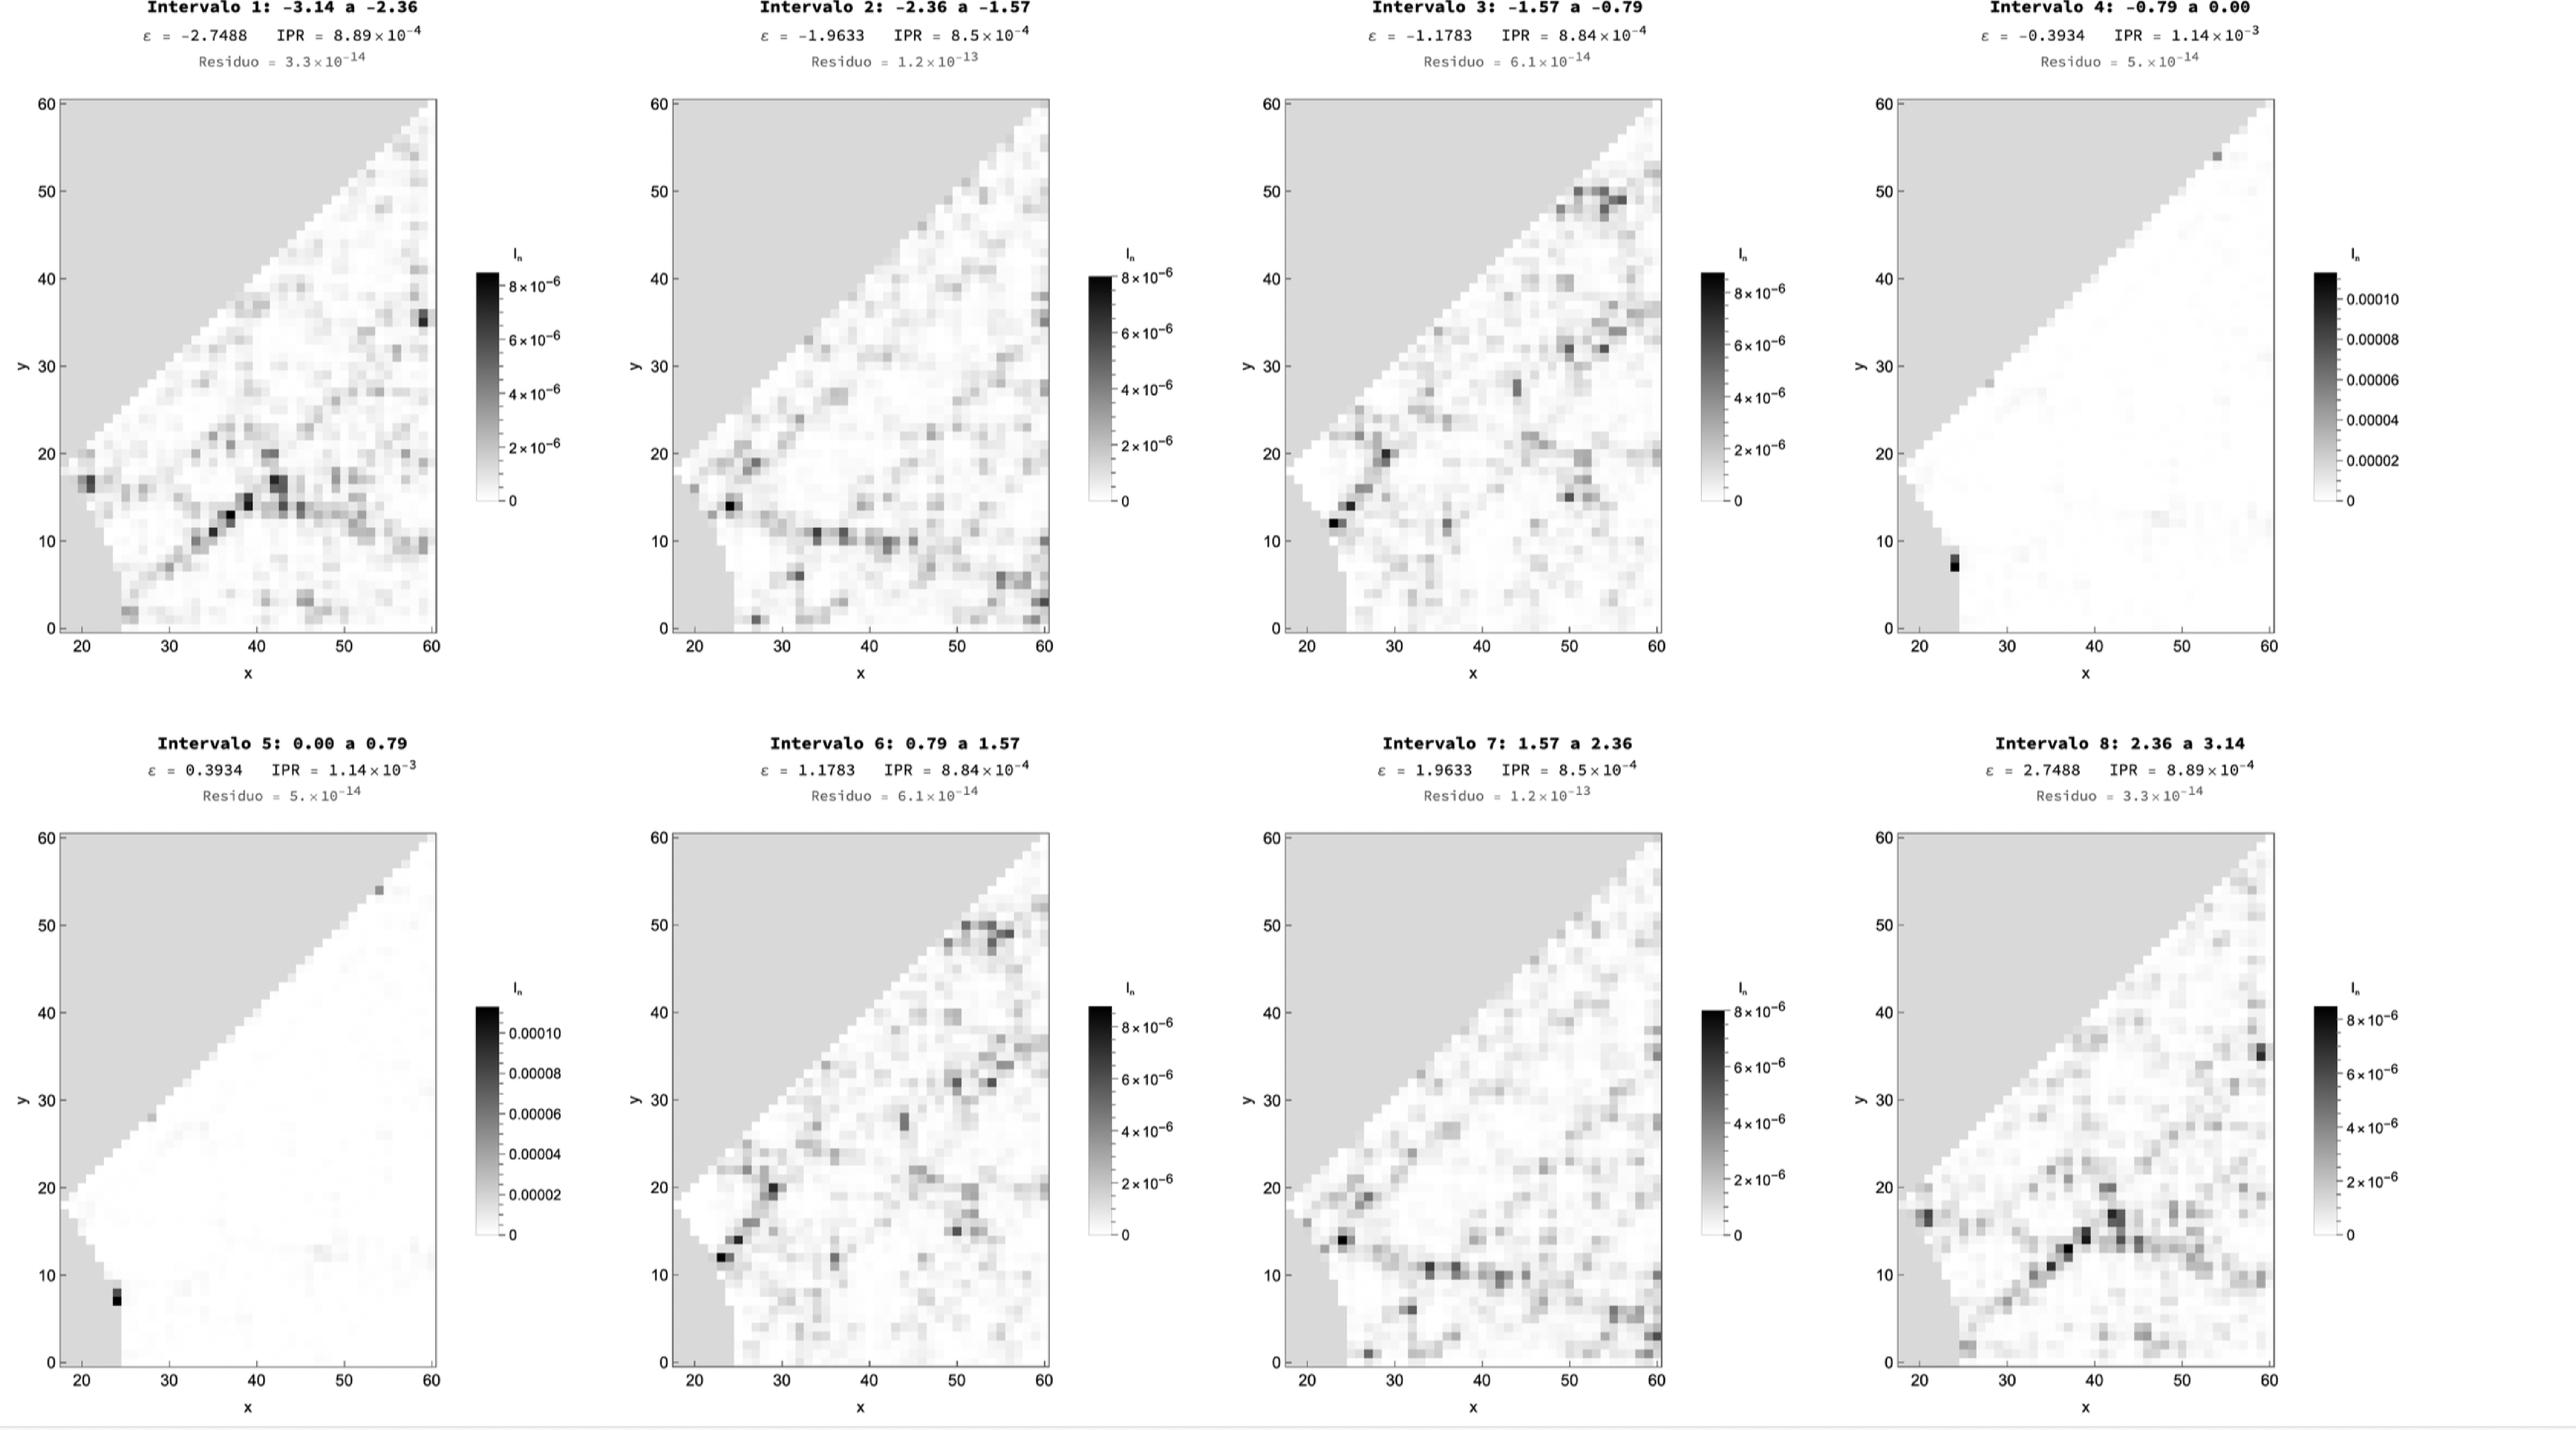
\includegraphics[width=\textwidth,height=5.7cm,keepaspectratio]{IPRDensity_Sinai_Intervals01-08.pdf}
  \captionline{Cada panel indica eigenfase, IPR y residuo numérico. Cada mapa tiene su propia escala.}
\end{frame}

\section{Apéndice de monedas}
\begin{frame}[t]{Matrices fijas de las monedas}
  \[
    G=\frac12\begin{pmatrix}
      -1&1&1&1\\1&-1&1&1\\1&1&-1&1\\1&1&1&-1
    \end{pmatrix},\qquad
    B=\frac1{\sqrt2}\begin{pmatrix}
      1&1&0&0\\0&0&1&1\\0&0&1&-1\\1&-1&0&0
    \end{pmatrix}.
  \]
  \captionline{Definiciones de \texttt{RandomMatrix} en el código del proyecto. Las conjugaciones usan $V^\dagger$ y preservan los eigenvalores de la moneda.}
  \takeaway{La orientación de la moneda respecto a $S$ también participa en la dinámica de $U$.}
\end{frame}
\fi

\end{document}
